\chapterimage{chap1.jpg}
\chapter{预备知识}
\begin{introduction}
	\item 函数定义和性质
	\item 基本不等式
	\item 柯西不等式
	\item 三角函数和反三角函数
	\item 特殊函数
\end{introduction}
\section{函数}
\begin{definition}[函数]
	1. 函数定义:
	
	$X,Y$ 是给定的两个集合, 若对于任意 $x\in X$, 存在法则 $f$, 使得唯一的 $y = f(x)$ 满足 $y\in Y$, 则称 $f$ 为从 $X$ 到 $Y$ 的一个函数, 记为 $f:X\to Y$, 其中 $X$ 称为定义域, $f(x)(x\in X)$ 称为值域
	
	2. 函数的三要素: 定义域、对应法则和值域
\end{definition}

\begin{definition}[函数的基本性质]
	\begin{enumerate}
		\item 单射: 若对于任意 $x_{1},x_{2}\in X$, 若 $x_{1}\neq x_{2}$, 则 $f(x_{1})\neq f(x_{2})$
		\item 满射: 若对于任意 $y\in Y$, 存在 $x\in X$, 使得 $f(x)=y$
		\item 双射: 若 $f$ 既是单射又是满射
	\end{enumerate}
\end{definition}

\begin{definition}[函数基本运算]
	\begin{enumerate}
		\item 基本四则运算
		\item 复合运算
		\item 反函数运算
	\end{enumerate}
\end{definition}

\begin{property}[函数四大性质]
	\begin{itemize}
		\item 有界性
		\item 奇偶性: $\begin{cases} \text{奇函数: }f(-x) = -f(-x) \\ \text{偶函数: }f(-x) = f(x) \end{cases}$
		\item 周期性: $f(x+T) = f(x)$
		\item 单调性: $\forall x_{1},x_{2}\in I (x_{1}\neq x_{2}),\dfrac{f(x_{1})-f(x_{2})}{x_{1}-x_{2}}>(<)0$, $f(x)$ 单调递增(减)
	\end{itemize}
\end{property}

\begin{corollary}[奇偶性推论]
	任意一个定义在 $[-l,l]$ 上的函数 $f(x)$ 均可以写成一个奇函数和一个偶函数的和 $f(x)=h(x)+g(x)$, 其中 $h(x)=\dfrac{f(x)+f(-x)}{2}$ 是偶函数, $g(x)=\dfrac{f(x)-f(-x)}{2}$ 是奇函数
\end{corollary}

\begin{corollary}[周期性、中心对称性、轴对称性]
	
	1. $f(x)$有对称中心$(a,c)$,且关于直线$x=b$轴对称,我们可以推出$f(x)$的一个周期$T=4|b-a|$.
	
	2. $f(x)$有两个对称中心$(a,c)$和$(b,c)$,我们可以推出$f(x)$的一个周期$T=2|b-a|$.
	
	3. $f(x)$有两个对称轴直线$x=a$和直线$x=b$,我们可以推出$f(x)$的一个周期$T=2|b-a|$.

\end{corollary}
\begin{anymark}[证明]
	1. 我们得到: 
	$$\begin{cases} f(2a-x)+f(x)=2c  \\ f(2b-x) = f(x)\end{cases}\to \begin{cases} f(2a-x) + f(2b-x) =2c\\ f(2a-2b+x) +f(x) =2c  \end{cases}\to f(x) = f(x+4a-4b)$$

	2. 我们得到:
	$$\begin{cases} f(2a-x) = f(2b-x)  \\ f(2a-2b+x) = f(x) \end{cases}\to f(x) = f(x+2a-2b)$$

	3. 我们得到:
	$$\begin{cases} f(2a-x) = f(x)  \\ f(2b-x) = f(x)\end{cases}\to \begin{cases} f(2a-x) = f(2b-x) \\ f(2a-2b+x) = f(x)   \end{cases}\to f(x) = f(x+2a-2b)$$
\end{anymark}

\subsection{初等函数}
\begin{definition}[初等函数]
	初等函数是指可以用有限次基本初等函数和有限次代数运算得到的函数, 六种基本初等函数:
	\begin{enumerate}
		\item 常数函数: $y=C$
		\item 幂函数: $y=x^{\alpha},\alpha\in \mathbb{R}^{*}$
		\item 指数函数: $y=a^{x},a>0,a\neq 1$
		\item 对数函数: $y=\log_{a}x,a>0,a\neq 1$
		\item 三角函数: $y=\sin x, y=\cos x, y=\tan x, y=\cot x, y=\sec x, y=\csc x$
		\item 反三角函数: $y=\arcsin x, y=\arccos x, y=\arctan x, y=\cot^{-1}(x), y=\sec^{-1}(x), y=\csc^{-1}(x)$
	\end{enumerate}
\end{definition}

\subsection{三角函数和反三角函数}
\begin{theorem}[积化和差\& 和差化积\& 倍角公式]
	积化和差公式:
	$$\sin\alpha\sin\beta=\dfrac{1}{2}[\cos(\alpha-\beta)-\cos(\alpha+\beta)]$$
	$$\cos\alpha\cos\beta=\dfrac{1}{2}[\cos(\alpha-\beta)+\cos(\alpha+\beta)]$$
	$$\sin\alpha\cos\beta=\dfrac{1}{2}[\sin(\alpha+\beta)+\sin(\alpha-\beta)]$$
	$$\cos\alpha\sin\beta=\dfrac{1}{2}[\sin(\alpha+\beta)-\sin(\alpha-\beta)]$$
	和差化积公式:
	$$\sin\alpha+\sin\beta=2\sin\dfrac{\alpha+\beta}{2}\cos\dfrac{\alpha-\beta}{2}$$
	$$\sin\alpha-\sin\beta=2\cos\dfrac{\alpha+\beta}{2}\sin\dfrac{\alpha-\beta}{2}$$
	$$\cos\alpha+\cos\beta=2\cos\dfrac{\alpha+\beta}{2}\cos\dfrac{\alpha-\beta}{2}$$
	$$\cos\alpha-\cos\beta=-2\sin\dfrac{\alpha+\beta}{2}\sin\dfrac{\alpha-\beta}{2}$$
	倍角公式:
	$$\sin 2\alpha = 2\sin\alpha\cos\alpha$$
	$$\cos 2\alpha = \cos^{2}\alpha-\sin^{2}\alpha = 2\cos^{2}\alpha-1 = 1-2\sin^{2}\alpha$$
	$$\tan 2\alpha = \dfrac{2\tan\alpha}{1-\tan^{2}\alpha}$$
	$$\sin 2\alpha = \dfrac{2\tan \alpha}{1+\tan^{2}\alpha}\qquad \qquad \cos 2\alpha = \dfrac{1-\tan^{2}\alpha}{1+\tan^{2}\alpha}$$
	$$\sin 3\alpha = 3\sin \alpha -4\sin^{3}\alpha\qquad\qquad \cos 3\alpha = 4\cos^{3}\alpha -3\cos \alpha$$
\end{theorem}
\begin{definition}[反三角函数]
	\begin{enumerate}
		\item $\arcsin x$ 的定义域为 $[-1,1]$, 值域为 $[-\dfrac{\pi}{2},\dfrac{\pi}{2}]$
		\item $\arccos x$ 的定义域为 $[-1,1]$, 值域为 $[0,\pi]$
		\item $\arctan x$ 的定义域为 $(-\infty,+\infty)$, 值域为 $(-\dfrac{\pi}{2},\dfrac{\pi}{2})$
	\end{enumerate}
\end{definition}
\begin{figure}[H]
	\centering  %图片全局居中
	\subfigure[$\arcsin(x)\ \&\ \sin (x)$]{
	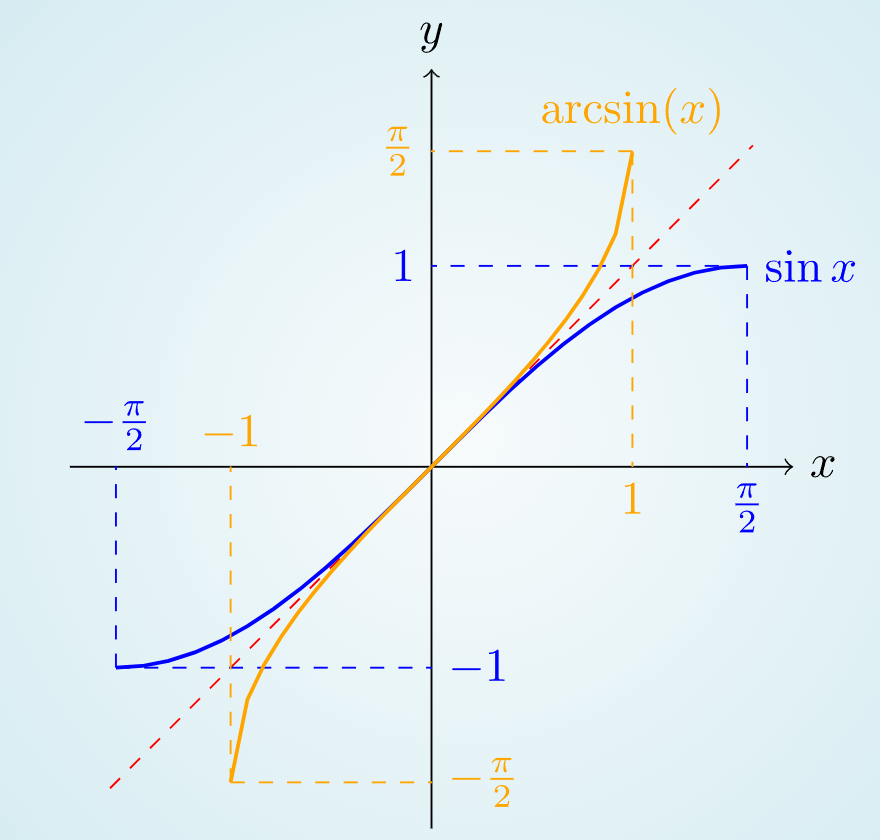
\includegraphics[width=0.4\textwidth]{"figure/Note/arcsinx.png"}}
	\subfigure[$\arccos(x)\ \&\ \cos (x)$]{
	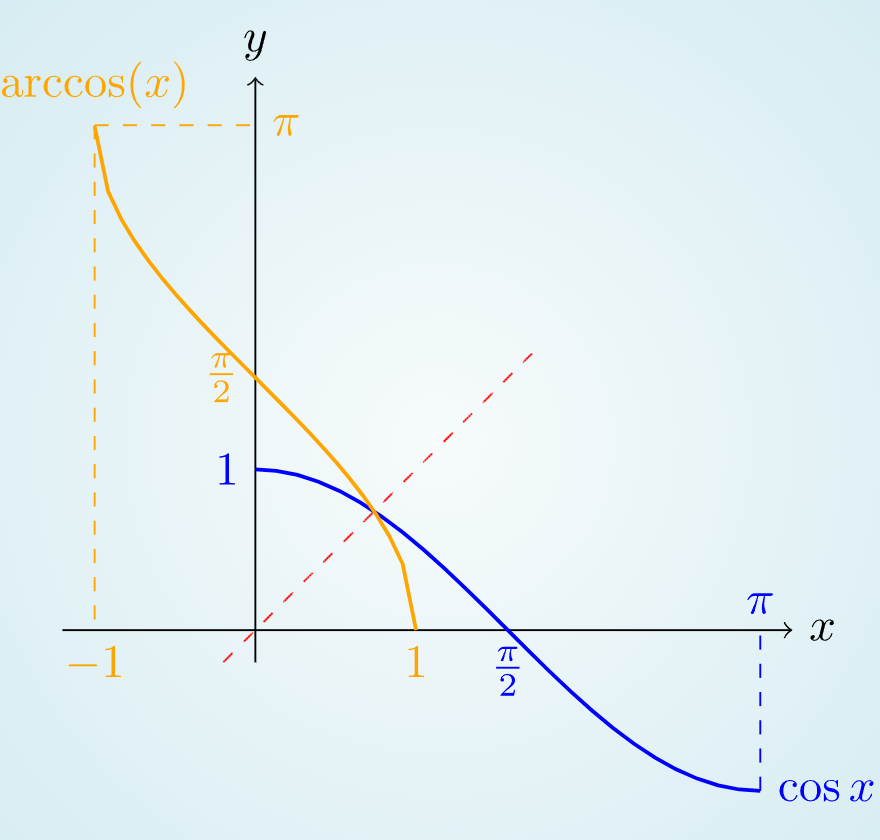
\includegraphics[width=0.4\textwidth]{"figure/Note/arccosx.png"}}
	\subfigure[$\arctan(x)\ \&\ \tan (x)$]{
	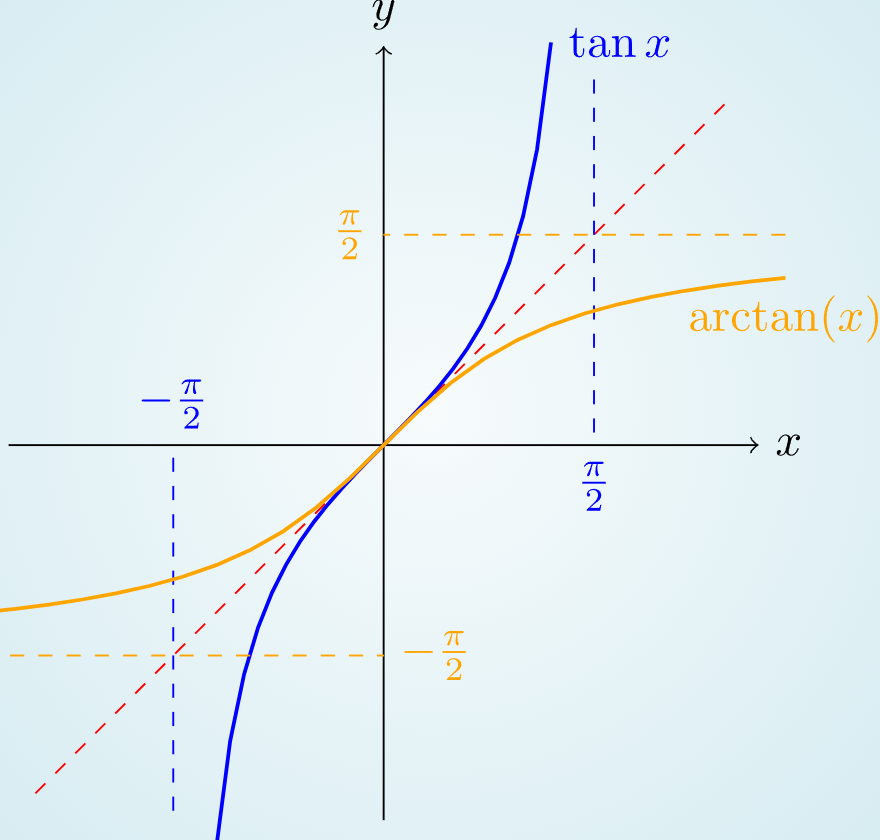
\includegraphics[width=0.4\textwidth]{"figure/Note/arctanx.png"}}
	\caption{反三角函数图像}
\end{figure}
\subsection{特殊函数}
\begin{definition}[特殊函数]
	\begin{enumerate}
		\item 阶乘函数: $$n!=n(n-1)(n-2)\cdots 2\cdot 1, (2n)!! = 2^{n}\cdot n!, 0! = 1$$
		\item 二项式系数: $$\binom{n}{k}=\dfrac{n!}{k!(n-k)!}, (a+b)^{n} = \sum\limits_{i = 0}^{n}\binom{n}{i}a^{i}b^{n-i}$$
		\item 绝对值函数: $$|x|=\begin{cases} x & x\geq 0 \\ -x & x<0 \end{cases}$$
		\item 符号函数: $$sgn(x)=\begin{cases} 1 & x>0 \\ 0 & x=0 \\ -1 & x<0 \end{cases}$$%
		\item 取整函数: $$f(x) = [x], x-1< [x] \leq x, \lim\limits_{x\to 0^{+}} = 0, \lim\limits_{x\to 0^{-}} =-1$$
		\item 分段函数: $$f(x)=\begin{cases} f_{1}(x) & x\in D_{1} \\ f_{2}(x) & x\in D_{2} \\ \cdots \end{cases}$$
		\item 黎曼函数:$$f(x)=\begin{cases} \dfrac{1}{q} & p,q\in \mathbb{Q}, x = \dfrac{p}{q}\in(0,1) \\ 0 & x\notin \mathbb{Q}, x=0,1 \end{cases}$$
		\item 狄利克雷函数: $$f(x)=\begin{cases} 1 & x\in \mathbb{Q} \\ 0 & x\notin \mathbb{Q} \end{cases}$$
	\end{enumerate}
\end{definition}


\begin{theorem}[平均值不等式 $a_{i} > 0$]
	平方平均值:
	$$Q_{n}=\sqrt{\dfrac{\sum\limits_{k=1}^{n}a_{k}^{2}}{n}}$$
	算术平均值:
	$$A_{n}=\dfrac{\sum\limits_{i=1}^{n}a_{i}}{n}$$
	几何平均值:
	$$G_{n}=\sqrt[n]{\prod\limits_{i=1}^{n}a_{i}}$$
	调和平均值:
	$$H_{n}=\dfrac{n}{\sum\limits_{i=1}^{k}\dfrac{1}{a_{i}}}$$
	平均值不等式:
	$$Q_{n}\geq A_{n}\geq G_{n}\geq H_{n}, a_{1} = a_{2} = \cdots = a_{n} \text{等号成立}$$
\end{theorem}

\begin{theorem}[柯西不等式]
	二维形式:
	$$(a^{2}+b^{2})(c^{2}+d^{2})\geq (ac+bd)^{2}, \text{当且仅当} ad =bc \text{时等号成立}$$
	$n$ 维形式:
	$$\left(\sum_{i=1}^{n}a_{i}b_{i}\right)^{2}\leq \left(\sum_{i=1}^{n}a_{i}^{2}\right)\left(\sum_{i=1}^{n}b_{i}^{2}\right),\text{当且仅当} \dfrac{a_{i}}{b_{i}}=c\text{时等号成立}$$
	$$\text{向量形式: } (\alpha,\beta)^{2}\leq (\alpha,\alpha)(\beta,\beta)$$
\end{theorem}
\begin{theorem}[重要不等式]
	\begin{enumerate}
		\item $\sin x < x < \tan x, x\in (0,\dfrac{\pi}{2})\qquad \qquad \arctan x < x < \arcsin x, x\in[0,1]$
		\item $\dfrac{2}{\pi}x < \sin x < x, x\in(0,\dfrac{\pi}{2})\qquad \qquad x < \tan x < \dfrac{4}{\pi}x , x\in(0,\dfrac{\pi}{4})$
		\item $e^{x} \geq x + 1,x\in\mathbb{R}\qquad \qquad x-1 \geq \ln x, x\in(0,+\infty)$
		\item $\dfrac{1}{1+x} < \ln (1+\dfrac{1}{x}) < \dfrac{1}{x}, x\in(0,+\infty)$
	\end{enumerate}
\end{theorem}

\begin{theorem}[重要公式]
	\begin{enumerate}
		\item $\dfrac{n}{(n+1)!} = \dfrac{1}{n!} - \dfrac{1}{(n+1)!}$
		\item $(a^{3}-b^{3}) = (a-b)(a^{2}+ab+b^{2})\qquad\qquad (a^{3}+b^{3}) = (a+b)(a^{2}-ab+b^{2})$
		\item $a^{n} - b^{n} = (a-b)(a^{n-1}-a^{n-2}b+\cdots -ab^{n-2}+b^{n-1})$
		\item $a^{n} + b^{n} = (a+b)(a^{n-1}-a^{n-1}b+\cdots -ab^{n-2} +b^{n-1}), n\in \{2k+1 | k\in \mathbb{N}\}$
	\end{enumerate}
\end{theorem}

\section{函数的表示方法}
\subsection{显式表达}
\begin{definition}[显示表达]
	$y = f(x)$ 的形式, 初等函数都是显性表达.
\end{definition}
\subsection{隐式表达}
\begin{definition}[隐式表达]
	$f(x,y) = 0$ 的形式, 一般不能用 $x$ 表示 $y$, 也不能用 $y$ 表示 $x$
\end{definition}
\subsection{极坐标}
\begin{definition}[极坐标]
	极坐标系是平面直角坐标系的一种推广, 它是由一个原点 $O$ 和一个射线 $Ox$ 组成的, 其中 $O$ 称为极点, $Ox$ 称为极轴, 任意一点 $P$ 到极点 $O$ 的距离 $r$ 叫做点 $P$ 的极径, 点 $P$ 到极轴的角 $\theta$ 叫做点 $P$ 的极角, 记为 $P(r,\theta)$
\end{definition}

\begin{definition}[重要极坐标方程]
	\begin{enumerate}
		\item 圆方程: $r = a, r = a\sin\theta, r = a\cos\theta$
		\item 心形线方程: $r = a(1\pm \cos\theta), r = a(1\pm \sin\theta)$
		\item 阿基米德螺线方程: $r = a\theta$
		\item 三叶玫瑰线方程: $r = a\sin 3\theta, r = a\cos 3\theta$
		\item 伯努利双扭线方程: $r^{2} = a^{2}\cos 2\theta, r^{2} = a^{2}\sin 2\theta$
	\end{enumerate}
\end{definition}
\subsection{参数方程}
\begin{definition}[参数方程]
	设 $x=x(t),y=y(t)$, 如果 $x,y$ 都是 $t$ 的函数, 那么称 $x=x(t),y=y(t)$ 为参数方程, $t$ 称为参数
\end{definition}
\begin{definition}[重要参数方程]
	\begin{enumerate}
		\item 摆线方程: $x = a(t-\sin t), y = a(1-\cos t)$
		\item 星形线方程: $x = a\cos^{3} t, y = a\sin^{3} t$
	\end{enumerate}
\end{definition}

\begin{anymark}[注]
	1. 关于双曲函数以及反双曲函数, 在 $\mathbf{def:}$ \ref{def: 双曲函数} 有详细介绍
	
	2. 有关极坐标和参数方程常见曲线的方程, 在 $\mathbf{def:}$ \ref{def: 常用曲线} 有详细介绍 
\end{anymark}




\chapterimage{chap2.jpg}

\chapter{数列极限}
\begin{introduction}
	\item 数列极限定义和性质
	\item 归结原理
	\item 夹逼准则
	\item 单调有界准则
\end{introduction}
\section{数列极限}
\begin{definition}[数列极限]
	设 $x_{n}$ 是 一数列, 若存在常数 $a$, $\forall \epsilon>0$, $\exists N_{0}>0$, 当 $n>N_{0}$ 时, $|x_{n}-a|<\epsilon$ 恒成立, 常数 $a$ 是数列 $\{x_{n}\}$ 的极限或者说数列 $\{x_{n}\}$ 趋近于 $a$
\end{definition}


\begin{property}[唯一性]
	若极限存在, 则极限唯一
\end{property}

\begin{property}[有界性]
	若数列 $\{x_{n}\}$ 的极限 $a$ 存在, 则数列 $\{x_{n}\}$ 有界
\end{property}

\begin{property}[保号性]
	若数列 $\{x_{n}\}$ 的极限 $a>0(a<0)$, 则存在正整数 $N_{0}$, 当 $n>N_{0}$ 时, $x_{n}>0(x_{n}<0)$, 取 $\epsilon = \pm a$ 即可
\end{property}
\begin{anymark}[注]
	1. 若数列的任意子列发散, 数列极限不存在

	2. 若数列的任意两个子列极限存在但不相等, 数列极限不存在
\end{anymark}
\begin{corollary}[数列极限]
	\begin{itemize}
		\item 如果数列从某项起有 $x_{n}\geq 0$ 且 $\lim\limits_{n\to\infty}x_{n} = a$, 则 $a\geq 0$
		\item 如果 $\lim\limits_{n\to\infty} x_{n} = A$, 则 $\lim\limits_{n\to\infty} |x_{n}| = |A|$
		\item $\lim\limits_{n\rightarrow +\infty}x_{n}=a\to \begin{cases} \lim\limits_{n\rightarrow +\infty}\dfrac{x_{n+1}}{x_{n}}=1, & a\neq 0\\ \lim\limits_{n\rightarrow +\infty}\dfrac{x_{n+1}}{x_{n}} \text{不一定存在}, & a=0  \end{cases}$
		\item $\lim\limits_{n\rightarrow +\infty}\dfrac{x_{n+1}}{x_{n}}=a\to \begin{cases} \lim\limits_{n\rightarrow +\infty}x_{n}=\infty,& |a|>1  \\ \lim\limits_{n\rightarrow +\infty}x_{n}=0,&|a|<1\\  \lim\limits_{n\rightarrow +\infty}x_{n}\text{不确定},&|a|=1 \end{cases}$
		\item $\lim\limits_{n\rightarrow +\infty}\dfrac{x_{n+1}}{x_{n}}\text{存在且}x_{n}>0\to \lim\limits_{n\rightarrow +\infty}\sqrt[n]{x_{n}}=\lim\limits_{n\rightarrow +\infty}\dfrac{x_{n+1}}{x_{n}}$
	\end{itemize}
\end{corollary}

\section{数列极限计算}
\subsection{定义法}
\begin{definition}[极限的四则运算]
	$$\lim\limits_{n\to \infty}x_{n}=a,\lim\limits_{n\to \infty}y_{n}=b$$
	\begin{enumerate}
		\item $\lim\limits_{n\to \infty}(x_{n}\pm y_{n}) = a\pm b$
		\item $\lim\limits_{n\to \infty}(x_{n}\cdot y_{n}) = a\cdot b$
		\item $\lim\limits_{n\to \infty}\dfrac{x_{n}}{y_{n}} = \dfrac{a}{b}, b\neq 0$
	\end{enumerate}

\end{definition}
\subsection{归结原理}
\begin{definition}[归结原理]
	设函数 $f(x)$ 在去心邻域 $\mathring{U}(a,\delta)$ 上有定义, 那么 $\lim\limits_{x\to a}f(x) = l$ 的充分必要条件是: 对与一切序列 $\{x_{n}\}_{n=1}^{\infty}\subset \mathring{U}(a,\delta)$, 只要 $\lim\limits_{n\to\infty}x_{n}=a$, 就有 $\lim\limits_{n\to\infty}f(x_{n})=l$
\end{definition}
\subsection{夹逼准则}
\begin{definition}[夹逼准则]
	设数列 $\{x_{n}\}$, $\{y_{n}\}$, $\{z_{n}\}$ 满足 $x_{n}\leq y_{n}\leq z_{n}$, $\lim\limits_{n\to\infty}x_{n}=\lim\limits_{n\to\infty}z_{n}=a$, 则 $\lim\limits_{n\to\infty}y_{n}=a$, 条件可变为 $n>N_{0}$ 时, $x_{n}\leq y_{n}\leq z_{n}$(有限无关性)
\end{definition}

\begin{corollary}[夹逼准则]
	$\lim\limits_{n\rightarrow +\infty}\sqrt[n]{u_{1}^{n}+u_{2}^{n}+u_{3}^{n}+\cdots+u_{m}^{n}}=\max\{ u_{1},u_{2},\cdots,u_{m}\}$
	\begin{anymark}[证明]
		$$[\max\{ u_{1},u_{2},\cdots,u_{m}\}]^{n}\leq u_{1}^{n}+u_{2}^{n}+u_{3}^{n}+\cdots+u_{m}^{n}\leq m[\cdot\max\{ u_{1},u_{2},\cdots,u_{m}\}]^{n}$$
	
		我们将$[\max\{ u_{1},u_{2},\cdots,u_{m}\}]^{n}$记作$a$,$m\cdot[\max\{ u_{1},u_{2},\cdots,u_{m}\}]^{n}$记作$b$,我们利用夹逼准则:

	$$\lim\limits_{n\rightarrow +\infty}\sqrt[n]{a}=\lim\limits_{n\rightarrow +\infty}\sqrt[n]{b}=\text{max}\{ u_{1},u_{2},\cdots,u_{m}\}$$
	\end{anymark}
\end{corollary}

\subsection{单调有界准则}
\begin{definition}[单调有界准则]
	单调有界数列必有极限, 详细证明见 $\mathbf{the:}$ \ref{the: 柯西收敛准则}.
\end{definition}
\section{Exercise}
\begin{proposition}
	设$x_{1}=a\geq 0$,$y_{1}=b\geq 0$,$a\leq b$,$x_{n+1}=\sqrt{x_{n}y_{n}},y_{n+1}=\dfrac{x_{n}+y_{n}}{2},(n=1,2,\cdots)$,证明:  $\lim\limits_{n\rightarrow +\infty}x_{n}=\lim\limits_{n\rightarrow +\infty}y_{n}$
\end{proposition}
\begin{solution}
	
	我们由:  $x_{1}=a\geq 0$,$y_{1}=b\geq 0$,$x_{n+1}=\sqrt{x_{n}y_{n}},y_{n+1}=\dfrac{x_{n}+y_{n}}{2}$,由归纳法可知:  
	$$x_{n}\geq 0, y_{n}\geq 0$$
	
	由基本不等式:  
	$$\dfrac{x_{n}+y_{n}}{2}\geq \sqrt{x_{n}y_{n}}\Rightarrow y_{n+1}\geq x_{n+1}$$
	
	又因为:  $x_{n+1}=\sqrt{x_{n}y_{n}}\geq x_{n}, y_{n+1}=\dfrac{x_{n}+y_{n}}{2}\leq y_{n}$.
	
	$x_{n}$单调递增,$y_{n}$单调递减,$x_{1}\leq x_{n}\leq y_{n}\leq y_{1}$
	
	$x_{n},y_{n}$单调且有界,数列$\{x_{n}\},\{y_{n}\}$均有极限,我们不妨设:  
	$$\left\lbrace
	\begin{array}{l}
		\lim\limits_{n\rightarrow +\infty}x_{n}=a\\
		\lim\limits_{n\rightarrow +\infty}y_{n}=b
	\end{array}
	\right. \Rightarrow \left\lbrace
	\begin{array}{l}
		a=\sqrt{ab}\\
		b=\dfrac{a+b}{2}
	\end{array}
	\right. \Rightarrow a=b$$
	
	综上所述,我们得到:  $\lim\limits_{n\rightarrow +\infty}x_{n}=\lim\limits_{n\rightarrow +\infty}y_{n}$
\end{solution}

\begin{proposition}
	设数列$\{a_{n}\}$满足$\lim\limits_{n\rightarrow+\infty}\dfrac{a_{n+1}}{a_{n}}=q$,且$|q|<1$,证明:  $\lim\limits_{n\rightarrow+\infty}a_{n}=0$
\end{proposition}
\begin{solution}
	
	我们考虑数列$\{|a_{n}|\}$,我们可以得到:  
	$$\lim\limits_{n\rightarrow +\infty}\dfrac{|a_{n+1}|}{|a_{n}|}=|q|\Rightarrow \exists\ M>0,\ n>M\text{时}, \dfrac{|a_{n+1}|}{|a_{n}|}<1$$
	
	又因为$|a_{n}|\geq 0$,我们可以知道$\{|a_{n}|\}$极限必定存在,我们不妨假设$\lim\limits_{n\rightarrow+\infty}|a_{n}|=a$.
	
	假设$a\neq 0$,我们可以得到:  $$\lim\limits_{n\rightarrow  +\infty}\dfrac{|a_{n+1}|}{|a_{n}|}=\dfrac{\lim\limits_{n\rightarrow  +\infty}|a_{n+1}|}{\lim\limits_{n\rightarrow  +\infty}|a_{n}|}=1$$
	
	这和$|q|<1$矛盾!!!
	
	
	综上所述,我们可以得到:  $\lim\limits_{n\rightarrow+\infty}a_{n}=0$
\end{solution}

\begin{proposition}
	设$f_{n}(x)=1-(1-\cos x)^n(n=1,2,\cdots)$

(1). 证明:  方程$f_{n}(x)=\dfrac{1}{2}$在$(0,\dfrac{\pi}{2})$内有且只有一个实数根$x_{n}$

(2). 设$x_{n}\in(0,\dfrac{\pi}{2})$,满足$f_{n}(x)=\dfrac{1}{2}$,证明:  $$\arccos \dfrac{1}{n}<x_{n}<\dfrac{\pi}{2},\text{且}\lim\limits_{n\rightarrow +\infty}x_{n}=\dfrac{\pi}{2}$$
\end{proposition}
\begin{solution}
	
	我们构造辅助函数:  $G_{n}(x)=\dfrac{1}{2}-(1-\cos x)^{n}$
	
	(1). $$G_{n}'(x)=-n\sin x(1-\cos x)^{n-1}$$
	
	当$x\in(0,\dfrac{\pi}{2})$,$G_{n}'(x)<0$,$\ G_{n}(x)$在$(0,\dfrac{\pi}{2})$单调递减.
	
	$$G_{n}(0)=\dfrac{1}{2}>0,\ G_{n}(\dfrac{\pi}{2})=-\dfrac{\pi}{2}<0$$
	
	我们根据零点定理,可以得到:  $\exists \text{唯一的}x_{n}\in(0,\dfrac{\pi}{2}),\ s.t. G_{n}(x_{n})=0$
	
	(2). 我们将$x=\arccos\dfrac{1}{n}$代入$G_{n}(x)$得到:  
	$$G_{n}(\arccos\dfrac{1}{n})=\dfrac{1}{2}-(1-\dfrac{1}{n})^{n}$$
	
	我们知道:  $\lim\limits_{n\rightarrow+\infty}(1-\dfrac{1}{n})^{n}=\dfrac{1}{e}\Rightarrow G_{n}(\arccos\dfrac{1}{n})>0$
	
	我们需要证明:  $(1-\dfrac{1}{n})^n$单调性,我们构造辅助函数:  $H(x)=e^{xln(1-\dfrac{1}{x})},x\geq 2$
	
	我们可以得到:  $H'(x)=e^{xln(1-\dfrac{1}{x})}[ln(1-\dfrac{1}{x})+\dfrac{1}{x-1}]>0$,$H(x)$单调递增.
	
	所以$G_{n}(\arccos\dfrac{1}{n})$单调递减,且$\lim\limits_{n\rightarrow+\infty}G_{n}(\arccos\dfrac{1}{n})=\dfrac{1}{2}-\dfrac{1}{e}>0$,我们得到:  $$\arccos \dfrac{1}{n}<x_{n}<\dfrac{\pi}{2}$$
	
	我们再由夹逼定理可以得到:  
	$$\left\lbrace
	\begin{array}{l}
		\lim\limits_{n\rightarrow  +\infty}\arccos \dfrac{1}{n}=\dfrac{\pi}{2}\\
		\lim\limits_{n\rightarrow  +\infty}\dfrac{\pi}{2}=\dfrac{\pi}{2}
	\end{array}
	\right. \Rightarrow \lim\limits_{n\rightarrow +\infty}x_{n}=\dfrac{\pi}{2}$$
	
\end{solution}

\begin{proposition}
	设$x_{1}>0$,数列$\{x_{n}\}$满足$x_{n+1}=ln(e^{x_{n}}-1)-ln x_{n}$,证明:  $\lim\limits_{n\rightarrow +\infty}x_{n}$存在并求其值
\end{proposition}
\begin{solution}
	
	我们由:  $x_{n+1}=ln(e^{x_{n}}-1)-ln x_{n}$可以得到:  
	$$e^{x_{n+1}}=\dfrac{e^{x_{n}}-1}{x_{n}}$$
	
	我们构造辅助函数$f(x)=e^x-x-1$,$f'(x)=e^{x}-1$
	
	当$x>0$时,我们知道:  $f'(x)>0$,$f(x)$单调递增,$f(x)>f(0)=0\Rightarrow  x>0,\dfrac{e^x-1}{x}>1$
	
	我们有$x_{1}>0\Rightarrow e^{x_{2}}>1\Rightarrow x_{2}>0$,我们由归纳法可知:  $x_{n}>0$,数列$\{ x_{n}\}$有下界.
	
	我们由拉格朗日中值定理可以得到:  
	$$e^{x_{n+1}}=\dfrac{e^{x_{n}}-1}{x_{n}}=e^{\xi},\text{其中}\xi\in(0,x_{n})$$
	
	我们得到:  $x_{n+1}=\xi<x_{n}$,数列$\{x_{n}\}$单调递减,我们由单调有界准则可以得到:  数列$\{x_{n}\}$极限必定存在,我们不妨假设$\lim\limits_{n\rightarrow +\infty}x_{n}=a$,我们有:  
	$$e^{a}=\dfrac{e^a-1}{a}\Rightarrow a=0$$
	
	综上所述,数列$\{x_{n}\}$极限存在,其值为$0$
\end{solution}
\begin{proposition}
	设$f(x)$在$[a,b]$上可导,且$|f'(x)|<1$,当$x\in[a,b]$时,有$a<f(x)<b$,$F(x)=\dfrac{x+f(x)}{2}$,证明:  

(1). $\exists x^{*}\in(a,b),\ s.t. F(x^{*})=x^{*}$

(2). 对$x_{0}\in[a,b]$,数列$\{x_{n}\}$满足$x_{n+1}=F(x_{n}),(n=0,1,2,\cdots)$,有$\lim\limits_{n\rightarrow+\infty}x_{n}=x^{*}$

\end{proposition}
\begin{solution}
	
	(1). 我们构造辅助函数:  $G(x)=F(x)-x=\dfrac{f(x)-x}{2}$,我们有:  $G'(x)=\dfrac{f'(x)-1}{2}$
	
	又因为:  $|f'(x)|<1\Rightarrow G'(x)<0\Rightarrow G(x)\text{单调递减}$
	$$\left\lbrace
	\begin{array}{l}
		G(a)=\dfrac{f(a)-a}{2}>0\\
		G(b)=\dfrac{f(b)-b}{2}<0
	\end{array}
	\right. \Rightarrow G(a)G(b)<0$$
	
	我们根据零点定理可知:  $\exists x^{*}\in(a,b),\ s.t. G(x^{*})=0\Rightarrow \exists x^{*}\in(a,b),\ s.t. F(x^{*})=x^{*}$
	
	(2). 
	$F'(x)=\dfrac{1+f'(x)}{2}\geq 0\Rightarrow F(x)\text{单调递增}$
	
	(i). 当$x_{0}=x^{*}$时,$x_{n}=x^{*}$,此时$\lim\limits_{n\rightarrow +\infty}x_{n}=x^{*}$
	
	(ii). 当$x_{0}>x^{*}$时,我们有$G(x^{*})>G(x_{0})\Rightarrow F(x_{0})<x_{0}\Rightarrow x_{1}<x_{0}$
	
	当$n=1$时,$x_{1}<x_{0}$;
	
	当$n=k$时,$x_{k}<x_{k-1}$成立,当$n=k+1$时,我们有$F(x_{k})<F(x_{k-1})\Rightarrow x_{k+1}<x_{k}$
	
	我们得到数列$\{x_{n}\}$单调递减,且$x_{0}\in[a,b],\ x_{n}=\dfrac{x_{n}+f(x_{n})}{2},\ a<f(x)<b\Rightarrow x_{n}\in[a,b]$,数列$\{x_{n}\}$单调递减且有下界,极限必定存在.
	
	我们不妨假设数列$\{x_{n}\}$的极限为$A$,我们有:  $A=\dfrac{A+f(A)}{2}\Rightarrow F(A)=A\Rightarrow A=x^{*}$
	
	(iii). 当$x_{0}<x_{*}$时,我们有$G(x^{*})<G(x_{0})\Rightarrow F(x_{0})>x_{0}\Rightarrow x_{1}>x_{0}$
	
	当$n=1$时,$x_{1}>x_{0}$;
	
	当$n=k$时,$x_{k}>x_{k-1}$成立,当$n=k+1$时,我们有$F(x_{k})>F(x_{k-1})\Rightarrow x_{k+1}>x_{k}$
	
	我们得到数列$\{x_{n}\}$单调递增,且$x_{0}\in[a,b],\ x_{n}=\dfrac{x_{n}+f(x_{n})}{2},\ a<f(x)<b\Rightarrow x_{n}\in[a,b]$,数列$\{x_{n}\}$单调递增且有上界,极限必定存在.
	
	我们不妨假设数列$\{x_{n}\}$的极限为$A$,我们有:  $A=\dfrac{A+f(A)}{2}\Rightarrow F(A)=A\Rightarrow A=x^{*}$
	
	综上所述,我们得到:  $\lim\limits_{n\rightarrow+\infty}x_{n}=x^{*}$
\end{solution}
\begin{proposition}
(1).设$f(x)$是$[0,+\infty)$上单调减少且非负的连续函数,证明:  $$f(k+1)\leq \int_{k}^{k+1}f(x)dx\leq f(k),\ k=1,2,\cdots$$

(2). 证明:  $ln(1+n)\leq 1+\dfrac{1}{2}+\cdots+\dfrac{1}{n}\leq 1+ln n$,求极限$\lim\limits_{n\rightarrow+\infty}\dfrac{1+\dfrac{1}{2}+\cdots+\dfrac{1}{n}}{ln n}$

\end{proposition}
\begin{solution}
	
	(1). 我们由$f(x)$单调减少且非负得到:  
	$$0\leq f(k+1)\leq f(x)\leq f(k),\ x\in[k,k+1]$$
	
	我们对上述不等式在$[k,k+1]$上同时求定积分得到:  
	$$\int_{k}^{k+1}f(k+1)dx\leq \int_{k}^{k+1}f(x)dx\leq \int_{k}^{k+1}f(k)dx\Rightarrow f(k+1)\leq \int_{k}^{k+1}f(x)dx\leq f(k)$$
	
	(2). 我们构造辅助函数$f(x)=\dfrac{1}{x}$,我们可以知道$f(x)$在$(0,+\infty)$上单调递减且非负,我们由(1)可以知道:  
	$$\left\lbrace
	\begin{array}{l}
		\dfrac{1}{2}\leq \int_{1}^{2}\dfrac{1}{x}dx\leq 1\\
		\dfrac{1}{3}\leq \int_{2}^{3}\dfrac{1}{x}dx\leq \dfrac{1}{2}\\
		\cdots\\
		\dfrac{1}{n}\leq \int_{n-1}^{n}\dfrac{1}{x}dx\leq \dfrac{1}{n-1}\\
		\dfrac{1}{n+1}\leq \int_{n}^{n+1}\dfrac{1}{x}dx\leq \dfrac{1}{n}
	\end{array}
	\right. \Rightarrow \left\lbrace
	\begin{array}{l}
		\sum\limits_{k=2}^{n+1}\dfrac{1}{k}\leq \int_{1}^{n+1}\dfrac{1}{x}=ln(1+n)\leq \sum\limits_{k=1}^{n}\dfrac{1}{k}\\
		\sum\limits_{k=2}^{n}\dfrac{1}{k}\leq \int_{1}^{n}\dfrac{1}{x}=ln n\\
		\sum\limits_{k=1}^{n}\dfrac{1}{k}=1+\sum\limits_{k=2}^{n}\dfrac{1}{k}\leq 1+ln n
	\end{array}
	\right. $$
	
	我们由夹逼定理可以得到:  
	$$\left\lbrace
	\begin{array}{l}
		\lim\limits_{n\rightarrow +\infty}\dfrac{ln(1+n)}{ln n}=1\\
		\lim\limits_{n\rightarrow +\infty}\dfrac{1+ln n}{ln n}=1
	\end{array}
	\right. \Rightarrow \lim\limits_{n\rightarrow  +\infty}\dfrac{1+\dfrac{1}{2}+\cdots+\dfrac{1}{n}}{ln n}=1$$
\end{solution}

\begin{proposition}
	设$f(x)$在$(a,b)$内连续,且$\lim\limits_{x\rightarrow a^{+}}f(x)=\lim\limits_{x\rightarrow b^{-}}f(x)=-\infty$,证明:  $f(x)$在$(a,b)$内有最大值
\end{proposition}
\begin{solution}
	
	我们不妨取$M=f(\dfrac{a+b}{2})$,我们有$\lim\limits_{x\rightarrow a^{+}}f(x)=\lim\limits_{x\rightarrow b^{-}}f(x)=-\infty$
	
	我们由极限定义可以得到:  
	$$\left\lbrace
	\begin{array}{l}
		\exists a<c<\dfrac{a+b}{2},\ x\in(a,c),\ s.t. f(x)\leq f(\dfrac{a+b}{2})\\
		\exists \dfrac{a+b}{2}<d<b,\ x\in(d,b),\ s.t. f(x)\leq f(\dfrac{a+b}{2})
	\end{array}
	\right. $$
	
	在闭区间$[c,d]$上,$f(x)$连续,$f(x)$必定有最大值为$f(\xi),\ \xi\in[c,d]$,且$f(\xi)\geq f(\dfrac{a+b}{2})$.在区间$(a,c)\cup (d,b)$上,我们有$f(x)\leq f(\dfrac{a+b}{2})$.
	
	综上所述,$f(x)$在区间$(a,b)$内有最大值.
\end{solution}


\chapterimage{chap3.jpg}
\chapter{函数极限和连续}
\begin{introduction}
	\item 函数极限定义和性质
	\item 无穷小概念和比阶
	\item 洛必达法则
	\item 连续和间断
\end{introduction}
\section{函数极限}
\begin{definition}[函数极限]
	设函数 $f(x)$ 在点 $x_{0}$ 的某个去心邻域 $\mathring{U}(x_{0},\delta)$ 内有定义, 如果存在常数 $A$, 对于任意给定的正数 $\epsilon$, 总存在正数 $\delta$, 使得当 $x$ 满足不等式 $0<|x-x_{0}|<\delta$ 时, 对应的函数值 $f(x)$ 都满足不等式 $|f(x)-A|<\epsilon$, 那么常数 $A$ 是当 $x$ 趋于 $x_{0}$ 时函数 $f(x)$ 的极限, 记作 $\lim\limits_{x\to x_{0}}f(x)=A$
\end{definition}

\begin{definition}[单侧极限]
	若函数 $f(x)$ 在点 $x_{0}$ 的左(右)邻域内有定义, 如果存在常数 $A$, 对于任意给定的正数 $\epsilon$, 总存在正数 $\delta$, 使得当 $x$ 满足不等式 $0<x-x_{0}<\delta$($0<x_{0}-x<\delta$)时, 对应的函数值 $f(x)$都满足不等式 $|f(x)-A|<\epsilon$, 那么常数 $A$ 是当 $x$ 趋于 $x_{0}$ 时函数 $f(x)$ 的左(右)极限, 记作 $\lim\limits_{x\to x_{0}^{-}}f(x)=A$($\lim\limits_{x\to x_{0}^{+}}f(x)=A$)
\end{definition}

\begin{definition}[无穷远极限]
	无穷远处极限(双侧,单侧只取一边): $f(x)$ 在 $(-\infty,-a)\cup(a,+\infty)$ 上有定义, $\forall \epsilon>0$, $\exists A>0$, 当 $|x|>A$ 时, $|f(x)-l|<\epsilon$, 我们称 $l$ 是当 $x$ 趋于无穷远时函数 $f(x)$ 的极限, 记作 $\lim\limits_{x\to\infty}f(x)=l$
\end{definition}
\begin{definition}[极限发散]
	1. 震荡发散: $\lim\limits_{x\to 0}\sin(\dfrac{1}{x})$ 反复震荡

	2. 左右极限存在但不相等: $\lim\limits_{x\to 0}[x]$

	3. 广义收敛: $f(x)$ 在 $x=a$ 的去心邻域 $\mathring{U}(a,\delta)$ 上有定义, $\forall X>0$, $\exists \delta>0$, 当 $0<|x-a|<\delta$ 时, $|f(x)|>X$, 则称 $f(x)$ 在 $x=a$ 处广义收敛
\end{definition}

\begin{property}[唯一性]
	若极限存在, 则极限唯一
\end{property}

\begin{property}[局部有界性]
	若函数 $f(x)$ 满足$\lim\limits_{x\to x_{0}}f(x)=A$, 则存在正数 $M>0$, 存在正数 $\delta>0$, 使得当 $x$ 满足不等式 $0<|x-x_{0}|<\delta$ 时, 对应的函数值 $f(x)$ 都满足不等式 $|f(x)|\leq M$
\end{property}

\begin{property}[局部保号性]
	若函数 $f(x)$ 满足 $\lim\limits_{x\to x_{0}}f(x)=A>(<)0$, 则存在正数 $\delta>0$, 使得当 $x$ 满足不等式 $0<|x-x_{0}|<\delta$ 时, 对应的函数值 $f(x)>(<)0$
\end{property}

\section{函数极限计算}
\subsection{无穷小(大)概念和比阶}
\begin{definition}[无穷小(大)]
	1. 无穷小: 设函数 $f(x)$ 在点 $x_{0}$ 的某个去心邻域 $\mathring{U}(x_{0},\delta)$ 内有定义, 如果 $\lim\limits_{x\to x_{0}}f(x)=0$, 那么称函数 $f(x)$ 是当 $x$ 趋于 $x_{0}$ 时的无穷小

	2. 无穷大: 设函数 $f(x)$ 在点 $x_{0}$ 的某个去心邻域 $\mathring{U}(x_{0},\delta)$ 内有定义, 如果 $\lim\limits_{x\to x_{0}}f(x)=\infty$, 那么称函数 $f(x)$ 是当 $x$ 趋于 $x_{0}$ 时的无穷大
\end{definition}

\begin{definition}[无穷小比阶]
	$$\lim\limits_{x\to 0}f(x)=\lim\limits_{x\to 0}g(x)=0$$

	1. 等价无穷小: $\lim\limits_{x\to 0}\dfrac{f(x)}{g(x)}=1$, 记作 $f(x)\sim g(x)$

	2. 同阶无穷小: $\lim\limits_{x\to 0}\dfrac{f(x)}{g(x)}=k(k\neq 0)$, 记作 $f(x)\approx g(x)$

	3. 高阶无穷小: $\lim\limits_{x\to 0}\dfrac{f(x)}{g(x)}=0$, 记作 $f(x)=o(g(x))$

	4. 低阶无穷小: $\lim\limits_{x\to 0}\dfrac{f(x)}{g(x)}=\infty$, 记作 $g(x)=O(f(x))$
\end{definition}

\begin{corollary}[等价无穷小]
	\begin{enumerate}
		\item $x\to 0, x\sim \sin x\sim \tan x\sim \arcsin x\sim \arctan x\sim \ln(x+1)\sim e^{x}-1$
		\item $x\to 0, \sin x\sim x - \dfrac{x^{3}}{6}, \arcsin x\sim x+\dfrac{x^{3}}{6}, \tan x\sim x+\dfrac{x^{3}}{3}, \arctan x\sim x-\dfrac{x^{3}}{3},\cos x\sim 1-\dfrac{x^{2}}{2}$
		\item $x\to 0, (1+x)^{a}-1\sim ax, a^{x}-1\sim x\ln a$
	\end{enumerate}
\end{corollary}
\begin{theorem}[洛必达法则]
	设函数 $f(x)$ 和 $g(x)$ 都在 $x=a$ 的某邻域内可导($a$ 可以为 $\infty$, 邻域也可以是单侧的), 且 $g'(a)\neq 0$, 满足:(1) 或 (2)

	(1). $\dfrac{0}{0}$: $\lim\limits_{x\to a}f(x)=\lim\limits_{x\to a}g(x)=0$

	(2). $\dfrac{\infty}{\infty}$: $\lim\limits_{x\to a}f(x)=\lim\limits_{x\to a}g(x)=\infty$

	如果 $\lim\limits_{x\to a}\dfrac{f'(x)}{g'(x)}=l$($l$ 可以是实数或者 $\infty$), 我们有: $\lim\limits_{x\to a}\dfrac{f(x)}{g(x)}=l$
\end{theorem}
\begin{anymark}[证明]
	构造辅助函数: $F(x) = \begin{cases} 0,& x=x_{0}  \\ f(x),&x\in\mathring{U}(x_{0}) \end{cases}, G(x)= \begin{cases} 0,& x=x_{0}  \\ g(x),&x\in\mathring{U}(x_{0}) \end{cases} $

	我们可以得到: $F(x),G(x)$ 在 $[x_{0},x]$ 上连续, 在 $(x_{0},x)$ 内可导, 且 $G'(x)\neq 0$
	
	我们利用柯西中值定理:
	
	$$\exists \xi\in (x_{0},x), s.t.\ \dfrac{F(x)-F(x_{0})}{G(x)-G(x_{0})}= \dfrac{F'(xi)}{G'(\xi)}\Rightarrow \dfrac{f(x)}{g(x)} = \dfrac{f'(\xi)}{g'(\xi)}$$

	我们取极限 $x\to x_{0}^{+}$ 得到: $\lim\limits_{x\to x_{0}^{+}}\dfrac{f(x)}{g(x)} = \lim\limits_{\xi\to x_{0}^{+}}\dfrac{f'(\xi)}{g'(\xi)} = \lim\limits_{x\to x_{0}^{+}}\dfrac{f'(x)}{g'(x)} $

	同理我们可以得到: $\lim\limits_{x\to x_{0}^{-}}\dfrac{f(x)}{g(x)} = \lim\limits_{x\to x_{0}^{-}}\dfrac{f'(x)}{g'(x)} $
	
	由于 $\lim\limits_{x\to a}\dfrac{f'(x)}{g'(x)}=l\to \lim\limits_{x\to x_{0}^{-}}\dfrac{f'(x)}{g'(x)} = \lim\limits_{x\to x_{0}^{+}}\dfrac{f'(x)}{g'(x)}=l$

	我们得到: $\lim\limits_{x\to x_{0}^{-}}\dfrac{f(x)}{g(x)} = \lim\limits_{x\to x_{0}^{+}}\dfrac{f(x)}{g(x)} = l$, 证毕
\end{anymark}
\begin{theorem}[广义洛必达定理]
	设 $f(x)$ 和 $g(x)$ 在 $\mathring{U}(x_{0})$ 上可导, 满足:

	(1). $g'(x)\neq 0$

	(2). $\lim\limits_{x\to x_{0}}g(x) =\infty$

	(3). $\lim\limits_{x\to x_{0}}\dfrac{f'(x)}{g'(x)}=A(A\text{为有限数或}\pm\infty)$

	我们有: $\lim\limits_{x\to x_{0}}\dfrac{f(x)}{g(x)}=A$
\end{theorem}
\begin{anymark}[证明]
	首先考虑 $x\to x_{0}^{-}$:

	(1). 当 $A$ 为常数时, 我们有:
	$$\forall \varepsilon > 0, \exists \delta > 0, s.t.\ x\in (x_{0}-\delta,x_{0}), |\dfrac{f'(x)}{g'(x)}-A|<\dfrac{\varepsilon}{3}\Rightarrow \text{取定} x_{1}\in (x_{0}-\delta,x_{0})$$

	我们考虑 $x\in (x_{1},x)$, 由柯西中值定理我们有:

	$$\dfrac{f(x)-f(x_{1})}{g(x)-g(x_{1})} = \dfrac{f'(\xi)}{g'(\xi)}\Rightarrow |\dfrac{f(x)-f(x_{1})}{g(x)-g(x_{1})}-A| = |\dfrac{f'(\xi)}{g'(\xi)}-A| < \dfrac{\varepsilon}{3}$$

	$x\in[x_{1},x_{0})$, 我们有:

	\begin{eqnarray*}
		|\dfrac{f(x)}{g(x)} -A| &=& |\dfrac{g(x)-g(x_{1})}{g(x)} \left[\dfrac{f(x)-f(x_{1})}{g(x)-g(x_{1})}-A\right] + \dfrac{f(x_{1})-Ag(x_{1})}{g(x)}|\\
								&\leq& |1-\dfrac{g(x_{1})}{g(x)}||\dfrac{f(x)-f(x_{1})}{g(x)-g(x_{1})}-A|+|\dfrac{f(x_{1})-Ag(x_{1})}{g(x)}|\\
								&\leq& (1+|\dfrac{g(x_{1})}{g(x)}|)|\dfrac{f(x)-f(x_{1})}{g(x)-g(x_{1})}-A|+|\dfrac{f(x_{1})-Ag(x_{1})}{g(x)}|
	\end{eqnarray*}

	我们有: $\lim\limits_{x\to x_{0}}g(x) =\infty\Rightarrow \begin{cases} \lim\limits_{x\to x_{0}}\dfrac{g(x_{1})}{g(x)} =0 \\ \lim\limits_{x\to x_{0}}\dfrac{f(x_{1})-Ag(x_{1})}{g(x)}=0\end{cases}$

	我们有:
	$$\forall \varepsilon >0, \exists x_{2}\in(x_{1},x_{0}),\forall x\in(x_{2},x_{0}),\ s.t.\ |\dfrac{g(x_{1})}{g(x)}|< 1 \text{且} |\dfrac{f(x_{1})-Ag(x_{1})}{g(x)}|< \dfrac{\varepsilon}{3}$$

	此时,我们有: $\forall \varepsilon > 0, \exists \delta_{1} = x_{0}-x_{2}, \forall x\in (x_{0}-\delta_{1},x_{0}), |\dfrac{f(x)}{g(x)} -A|<2\cdot \dfrac{\varepsilon}{3}+\dfrac{\varepsilon}{3}=\varepsilon$
	
	(2). 当 $A$ 为 $\infty$ 时, 我们有: $|\dfrac{f(x)-f(x_{1})}{g(x)-g(x_{1})}| = |\dfrac{f'(\xi)}{g'(\xi)}| > M$
	
	取 $M = 1\to |f(x)-f(x_{1})|>|g(x)-g(x_{1})|\to \lim\limits_{x\to x_{0}^{-}}f(x) = \infty$

	$x\to x_{0}^{+}$ 的情况类似, 证毕
\end{anymark}

\section{连续和间断}
\begin{definition}[连续点]
	设函数 $f(x)$ 在点 $x_{0}$ 的某个邻域 $U(x_{0},\delta)$ 内有定义, 如果 $\lim\limits_{x\to x_{0}}f(x)=f(x_{0})$, 那么称函数 $f(x)$ 在点 $x_{0}$ 处连续
\end{definition}

\begin{definition}[间断点]
	第一类间断点:
	\begin{enumerate}
		\item 可去间断点: $\lim\limits_{x\to x_{0}}f(x)\neq f(x_{0})$($f(x_{0})$ 可以无定义)
		\item 跳跃间断点: $\lim\limits_{x\to x_{0}^{-}}f(x)\neq \lim\limits_{x\to x_{0}^{+}}f(x)$
	\end{enumerate}

	第二类间断点: $\lim\limits_{x\to x_{0}^{-}}f(x)$ 和 $\lim\limits_{x\to x_{0}^{+}}f(x)$ 至少有一个不存在
	\begin{enumerate}
		\item 震荡间断点: $\lim\limits_{x\to x_{0}}f(x)$ 震荡不存在
		\item 无穷间断点: $\lim\limits_{x\to x_{0}}f(x)=\infty$
		\item 其他第二类间断点
	\end{enumerate}
\end{definition}
\chapterimage{chap4.jpg}
\chapter{一元微分学}
\begin{introduction}
	\item 导数和微分
	\item 基本求导公式
	\item 高阶导数
	\item 泰勒公式
	\item 函数单调性和凹凸性
	\item 极值点和拐点
	\item 渐近线
	\item 曲率和曲率半径
\end{introduction}

\section{一元微分学概念}
\begin{definition}[导数]
	设 $y=f(x)$ 定义在区间 $I$ 上, 自变量在 $x=x_{0}$ 处增加一个增量 $\Delta x$ 时, 其中 $x_{0}\in I, x_{0}+\Delta\in I$, 函数值的增量 $\Delta y=f(x_{0}+\Delta x)-f(x_{0})$, 如果极限 $\lim\limits_{\Delta x\to 0}\frac{\Delta y}{\Delta x}$ 存在, 那么称此极限为函数 $y=f(x)$ 在点 $x_{0}$ 处的导数, 记为 $f'(x_{0})$ 或 $\dfrac{dy}{dx}|_{x=x_{0}}$ 或 $\dfrac{df(x)}{dx}|_{x=x_{0}}$
\end{definition}
\begin{definition}[导数的几何意义]
	函数 $y=f(x)$ 在点 $x=x_{0}$ 处的导数 $f'(x_{0})$ 是函数 $y=f(x)$ 在点 $x=x_{0}$ 处的切线的斜率
\end{definition}

\begin{theorem}[导数存在充要条件]
	函数 $y=f(x)$ 在点 $x=x_{0}$ 处可导的充要条件是: 函数 $y=f(x)$ 在点 $x=x_{0}$ 处的左导数 $f'_{-}(x_{0})$ 和右导数 $f'_{+}(x_{0})$ 存在且相等
\end{theorem}

\begin{definition}[微分]
	设 $y=f(x)$ 定义在区间 $I$ 上, 如果函数 $y=f(x)$ 在点 $x_{0}$ 处可导, 那么函数 $y=f(x)$ 在点 $x_{0}$ 处的微分为 $dy=f'(x_{0})dx$, 其中 $dx$ 是自变量 $x$ 的增量, $dy$ 是因变量 $y$ 的增量
\end{definition}
\section{一元微分学计算}
\begin{theorem}[基本求导公式]
	\begin{enumerate}
		\item $(x^{\alpha})'= \alpha x^{\alpha-1}$
		\item $(a^{x})'= a^{x}\ln a \qquad\qquad (\log_{a}x)'= \dfrac{1}{x\ln a}$
		\item $(e^{x})'= e^{x}\qquad \qquad (\ln x)' = \dfrac{1}{x}$
		\myspace{1}
		\item $(\sin x)' = \cos x\qquad \qquad (\cos x)' = -\sin x$
		\item $(\tan x)' = \sec^{2} x = \dfrac{1}{\cos^{2} x}$
		\item $(\sec x)' = \dfrac{\sin x}{\cos^{2}x} = \tan x\sec x$
		\item $(\csc x)' = \dfrac{-\cos x}{\sin^{2} x} = -\cot x\csc x$
		\item $(\cot x)' = -\csc^{2} x$
		\myspace{1}
		\item $(\arcsin x)' = \dfrac{1}{\sqrt{1-x^{2}}}$
		\item $(\arccos x)' = -\dfrac{1}{\sqrt{1-x^{2}}}$
		\item $(\arctan x)' = \dfrac{1}{x^{2}+1}$
		\myspace{1}
		\item $\left(\ln(x+\sqrt{x^{2}+a})\right)' = \dfrac{1}{\sqrt{x^{2}+a}}$
		\item $\left(\ln(x+\sqrt{x^{2}-a})\right)' = \dfrac{1}{\sqrt{x^{2}-a}}$
	\end{enumerate}
\end{theorem}

\begin{theorem}[导数四则运算]
	\begin{enumerate}
		\item 和差法则: $[f(x)\pm g(x)]' = f'(x) \pm g'(x)$
		\item 积法则: $[f(x)g(x)]' = f'(x)g(x) + f(x)g'(x)$
		\item 商法则: $\left[\dfrac{f(x)}{g(x)}\right]' = \dfrac{f'(x)g(x) - f(x)g'(x)}{[g(x)]^{2}}$
		\item 复合函数求导: $F[G(x)]' = F[G(x)]'\cdot G'(x)$
	\end{enumerate}
\end{theorem}

\begin{theorem}[高阶导数]
	\begin{enumerate}
		\item $\sin^{(n)} x = \sin (x+\frac{n\pi}{2})\qquad \qquad\sin^{(n)}(ax+b) = a^{n} \sin(ax+b+\frac{n\pi}{2})$
		\item $\cos^{(n)} x = \cos (x+\frac{n\pi}{2})\qquad\qquad \cos^{(n)}(ax+b) = a^{n} \cos(ax+b+\frac{n\pi}{2})$
		\item $[\ln(1+x)]^{(n)} = (-1)^{n-1}\dfrac{(n-1)!}{(1+x)^{n}}\qquad\qquad [\ln(1+x)]^{(n)} = (-1)^{n-1}\dfrac{(n-1)!a^{n}}{(ax+b)^{n}}$
		\item $(\dfrac{1}{ax+b})^{(n)} = (-1)^{n-1}\dfrac{(n-1)!a^{n}}{(ax+b)^{n+1}}$
		\item 莱布尼茨公式: $(uv)^{n} = \sum\limits_{i=0}^{n}\binom{i}{n}u^{(i)}v^{(n-i)}$

	\end{enumerate}
\end{theorem}

\begin{theorem}[泰勒公式]
	\begin{enumerate}
		\item 欧拉公式: $e^{i\theta}=\cos \theta+i\sin\theta$
		\item $e^{x}=1+x+\dfrac{x^{2}}{2!}+\cdots+\dfrac{x^{n}}{n!}+\cdots, x\in(-\infty,+\infty)$
		\item $\sin x = x-\dfrac{x^{3}}{3!}+\dfrac{x^{5}}{5!}-\dfrac{x^{7}}{7!}+\cdots+(-1)^{2n+1}\dfrac{x^{2n-1}}{(2n-1)!}+\cdots, x\in(-\infty,+\infty)$
		\item $\cos x=1-\dfrac{x^{2}}{2!}+\dfrac{x^{4}}{4!}-\dfrac{x^{6}}{6!}+\cdots+(-1)^{2n-1}\dfrac{x^{2n-2}}{(2n-2)!}+\cdots, x\in(-\infty,+\infty)$
		\item $\tan x = x+\dfrac{x^{3}}{3}+\cdots=\sum\limits_{n=0}^{\infty}\dfrac{B_{2n}(-4)^{n}(1-4^{n})}{(2n)!}x^{2n-1}, x\in(-\dfrac{\pi}{2},\dfrac{\pi}{2})$
		\myspace{1}
		\item $\arcsin x = x+\dfrac{x^{3}}{6}+\cdots=\sum\limits_{n=0}^{\infty}\dfrac{(2n)!}{4^{n}(n!)^{2}(2n+1)}x^{2n+1}, x\in(-1,1)$
		\item $\arctan x = x-\dfrac{x^{3}}{3}+\cdots = \sum\limits_{n=0}^{\infty}\dfrac{(-1)^{n}}{2n+1}x^{2n+1}, x\in(-1,1)$
		\myspace{1}
		\item $\ln (1+x) = x-\dfrac{x^{2}}{2}+\cdots+(-1)^{n+1}\dfrac{x^{n}}{n}+\cdots, x\in(-1,1]$
		\item $\ln (1-x) =-x-\dfrac{x^{2}}{2}-\cdots-\dfrac{x^{n}}{n}+\cdots, x\in[-1,1)$
		\item $(1+x)^{\alpha} = 1+\alpha x+\dfrac{\alpha(\alpha-1)}{2!}x^{2}+\cdots+\dfrac{\alpha(\alpha-1)\cdots(\alpha-n+1)}{n!}x^{n}$
	\end{enumerate}
\end{theorem}

\begin{theorem}[特殊函数导函数]
1. 隐函数导数: 

$$F(x,y) = 0\Rightarrow F'(x,y) \cdot y'= 0$$

2. 指对数函数求导: 

$$\ln y =\ln f(x)\Rightarrow \frac{y'}{y} = \frac{f'(x)}{f(x)}\qquad\qquad y = a^{f(x)}\Rightarrow y = e^{f(x)\ln a}$$

3. 反函数导数: $x = \varphi(y),y=f(x)$ 记 $x_{y}' = \varphi'(y),y_{x}' = f'(x)$
\myspace{1}
(1). 一阶导数: $x_{y}' y_{x}' =1\Rightarrow \varphi'(y) = \dfrac{1}{f'(x)}$

(2). 二阶导数: $x_{yy}'' =-\dfrac{y_{xx}''}{(y_{x}')^{3}}\qquad\qquad y_{xx}'' = -\dfrac{x_{yy}''}{(x_{y}')^{3}}$
\myspace{1}
4. 参数方程导数: $x = x(t), y = y(t)$
\myspace{1}
(1). 一阶导数: $\dfrac{dy}{dx} = \dfrac{dy}{dt}\cdot \dfrac{dx}{dt} = \dfrac{y'(t)}{x'(t)}$

(2). 二阶导数: $\dfrac{d^{2}y}{dx^{2}} = \dfrac{\frac{dy}{dx}}{dx} = \dfrac{\frac{dy}{dx}}{dt}\cdot \dfrac{dx}{dt} = \dfrac{dx}{dx}\left[\dfrac{d^{2}y}{dt^{2}}\cdot \dfrac{dx}{dt}+\dfrac{d^{2}x}{dt^{2}}\cdot \dfrac{dy}{dt}\right]$
\end{theorem}

\section{一元微分学应用}
\subsection{几何应用}
\begin{definition}[函数图像要点]
	\begin{enumerate}
		\item 定义域(间断点)
		\item 奇偶性
		\item 渐近线(铅垂、水平、斜)
		\begin{anymark}[Points]
			(1). $$\begin{cases}\text{水平渐近线:} \lim\limits_{x\to\infty}f(x)=a\Rightarrow y=a\\
				\text{铅垂渐近线:} \lim\limits_{x\to a}f(x)=\infty\Rightarrow x=a \\
				\text{斜渐近线:} \lim\limits_{x\to\infty}\dfrac{f(x)}{x}=a, \lim\limits_{x\to\infty}f(x)-ax = b\Rightarrow y=ax+b
			\end{cases}$$
			(2). 在同一个趋向方向中水平渐近线和斜渐进线只能有一个

			(3). 间断点处看铅垂渐近线, $\pm \infty$ 处看水平渐近线和斜渐近线
		\end{anymark}
		\item 单调性和极值
		\item 凹凸性和拐点
	\end{enumerate}
\end{definition}

\subsection{函数单调性 \&凹凸性 \&极值点 \&拐点}
\begin{definition}[单调性]
	1. 设函数$f(x)$在区间$I$上有定义,如果对任意$x_{1},x_{2}\in I,x_{1}<x_{2}$,均有$f(x_{1})<f(x_{2})$,则称函数$f(x)$在区间$I$上是单调递增的;如果对任意$x_{1},x_{2}\in I,x_{1}<x_{2}$,均有$f(x_{1})>f(x_{2})$,则称函数$f(x)$在区间$I$上是单调递减的.

	2. 设函数$f(x)$在区间$I$上有定义,如果对任意$x_{1},x_{2}\in I,x_{1}<x_{2}$,均有$f(x_{1})\leq f(x_{2})$,则称函数$f(x)$在区间$I$上是单调不减的;如果对任意$x_{1},x_{2}\in I,x_{1}<x_{2}$,均有$f(x_{1})\geq f(x_{2})$,则称函数$f(x)$在区间$I$上是单调不增的.
\end{definition}

\begin{definition}[凹凸性]
	设函数$f(x)$在区间$I$上有定义
	
	1. 如果对任意$x_{1},x_{2}\in I,x_{1}<x_{2}$,均有$f(\dfrac{x_{1}+x_{2}}{2}) < \dfrac{f(x_{1})+f(x_{2})}{2}$,则称函数$f(x)$在区间$I$上是凹的
	
	2. 如果对任意$x_{1},x_{2}\in I,x_{1}<x_{2}$,均有$f(\dfrac{x_{1}+x_{2}}{2}) > \dfrac{f(x_{1})+f(x_{2})}{2}$,则称函数$f(x)$在区间$I$上是凸的

	3. 如果对任意$x_{1},x_{2}\in I,x_{1}<x_{2}$,均有$f(\lambda_{1}x_{1} +\lambda_{2} x_{2}) >(<)\lambda_{1}f(x_{1}) +\lambda_{2}f(x_{2})(\lambda_{1}>0, \lambda_{2}>0, \lambda_{1}+\lambda_{2} = 1)$,则称函数$f(x)$在区间$I$上是凸(凹)的
\end{definition}

\begin{definition}[极值点]
	设函数$f(x)$在点$x_{0}$的某邻域$U(x_{0})$内有定义,如果对去心邻域内任意$x$,均有$f(x)<f(x_{0})(\text{或}f(x)>f(x_{0}))$,我们称$f(x_{0})$是函数$f(x)$的一个极小值(或极大值).
\end{definition}
\begin{definition}[驻点]
	一阶导数为$0$的点称为驻点; 对于多元函数而言,驻点是一阶偏导数都为$0$的点.
\end{definition}

\begin{theorem}[极值点判别]
	第一充分条件:
	$$\begin{cases} f(x) \text{在} x_{0} \text{处连续, 且在} \mathring{U}(x_{0}) \text{内可导} \\
		 x\in(x_{0}-\delta,x_{0}),f'(x) > 0; x\in(x_{0},x_{0}+\delta), f'(x) < 0, f(x) \text{在} x= x_{0}\text{取极大值}\\
		 x\in(x_{0}-\delta,x_{0}),f'(x) < 0; x\in(x_{0},x_{0}+\delta), f'(x) > 0, f(x) \text{在} x= x_{0}\text{取极小值}\\
		 x\in(x_{0}-\delta,x_{0})\cup(x_{0},x_{0}+\delta), f'(x)\text{不变号}, x = x_{0} \text{不是极值点}
		\end{cases}$$

	第二充分条件:
	$$
	\begin{cases} f(x) \text{在} x_{0} \text{处二阶可导, 且} f'(x_{0}) = 0, f''(x_{0})\neq 0\\
	f''(x_{0}) > 0, f(x) \text{在} x= x_{0}\text{取极小值}\\
	f''(x_{0}) < 0, f(x) \text{在} x= x_{0}\text{取极大值}
	\end{cases}
	$$

	第三充分条件:
	$$
	\begin{cases} f(x) \text{在} x_{0} \text{处} n \text{阶可导, 且} f^{(m)}(x_{0}) = 0(m = 1,2,\cdots,n-1), f^{(n)}(x_{0}) \neq 0, n\in \{2k|k\in \mathbb{N}^{+}\}\\
	f^{(n)}(x_{0}) > 0, f(x) \text{在} x= x_{0}\text{取极小值}\\
	f^{(n)}(x_{0}) < 0, f(x) \text{在} x= x_{0}\text{取极大值}
	\end{cases}
	$$
\end{theorem}

\begin{definition}[拐点]
	连续函数$f(x)$在区间$I$上连续,$x_{0}$是区间的内点,当函数$f(x)$经过点$(x_{0},f(x_{0}))$时,函数的凹凸性发生改变,则称$(x_{0},f(x_{0}))$是函数$f(x)$的拐点.
\end{definition}

\begin{theorem}[拐点判别]
	第一充分条件:
	$$
	\begin{cases} f(x) \text{在} x_{0} \text{处连续, 且在} \mathring{U}(x_{0}) \text{内二阶可导}\\
		x\in(x_{0}-\delta,x_{0}),f''(x)<(>)0; x\in(x_{0},x_{0}+\delta),f''(x)>(<)0\\
		(x_{0},f(x_{0})) \text{是} f(x) \text{的拐点}
	\end{cases}
	$$

	第二充分条件:
	$$
	\begin{cases} f(x) \text{在} x_{0} \text{处三阶可导}\\
		f''(x_{0}) = 0, f'''(x_{0})\neq 0\\
		(x_{0},f(x_{0})) \text{是} f(x) \text{的拐点}
	\end{cases}
	$$

	第三充分条件:
	$$
	\begin{cases} f(x) \text{在} x_{0} \text{处} n \text{阶可导}\\
		f^{(m)}(x_{0}) = 0(m = 1,2,\cdots,n-1), f^{(n)}(x_{0}) \neq 0, n\in \{2k+1|k\in \mathbb{N}^{+}\}\\
		(x_{0},f(x_{0})) \text{是} f(x) \text{的拐点}
	\end{cases}
	$$
	
\end{theorem}
\begin{theorem}[多项式函数极值点和拐点个数]
	假设 $P_{n}(x)=\prod\limits_{i=1}^{k}(x-a_{i})^{p_{i}}$, 其中 $k_{1}$ 个 $p_{i}$ 为奇数(大于 $1$), $k_{2}$ 个 $p_{i}$ 为偶数, $k_{0}$ 个 $p_{i}=1$, 满足 $k_{0}+k_{1}+k_{2} = k$, 我们有:
		\begin{itemize}
			\item $P_{n}(x)$ 的极值点个数: $k-1+k_{2} = k_{0}+k_{1}+2k_{2}-1$
			\item $P_{n}(x)$ 的拐点个数: $k+2k_{1}+k_{2}-2 = k_{0}+3k_{1}+2k_{2}-2$
		\end{itemize}

		具体证明过程见: $\mathbf{the: }$\ref{the: 代数基本定理}
\end{theorem}
\begin{anymark}[注]
	\begin{itemize}
		\item 驻点是导数为$0$的点,不一定是极值点
		\item 极值点导数可能存在,也可能不存在;当导数存在时,$f'(x_{0})=0$
		\item 拐点处二阶导数可能存在,也可能不存在;当二阶导数存在时,$f''(x_{0})=0$
	\end{itemize}
\end{anymark}
\begin{definition}[曲率和曲率半径]

	设$y(x)$二阶可导,则曲线 $y=y(x)$ 在其上点 $(x_{0},y(x_{0}))$ 处的曲率公式表示为:
	$$k=\frac{|y''|}{[1+(y')^{2}]^{\frac{3}{2}}}$$

	曲率半径:
	$$R=\frac{1}{k}=\frac{[1+(y')^{2}]^{\frac{3}{2}}}{|y''|}$$
\end{definition}
\begin{anymark}[曲率半径推导]
	我们不妨设曲线上的任意一点 $C(x_{0},f(x_{0}))$, 这点的曲率圆半径为 $R$, 我们可以知道这个圆是 $C$ 点和周围两个点 $A(x_{0}-\delta,f(x_{0}-\delta)),B(x_{0}+\delta,f(x_{0}+\delta))$ 的外接圆, 且 $A,B$ 无线靠近 $C$

	我们利用等面积法来求出这个外接圆半径 $R$, 首先我们利用正弦定理得到:
	$$\dfrac{a}{\sin A} = \dfrac{b}{\sin B} = \dfrac{c}{\sin C} = 2R\Rightarrow S_{\Delta ABC} = \dfrac{abc}{R}$$

	我们利用向量法求出 $\Delta ABC$ 的面积:
	$$S_{\Delta ABC} = \dfrac{1}{2}|\mathbf{det}(\vec{a},\vec{b})| ,\begin{cases} \vec{a} = (\delta, f(x_{0})-f(x_{0}))\\ \vec{b} = (\delta,f(x_{0}+\delta)-f(x_{0})) \\ \vec{c}= (2\delta,f(x_{0}+\delta)-f(x_{0}-\delta))\end{cases} $$

	我们得到:
	$$\begin{cases} S = \dfrac{\sqrt{\delta^{2}+\left[f(x_{0})-f(x_{0}-\delta)\right]^{2}}\sqrt{\delta^{2}+\left[f(x_{0}+\delta)-f(x_{0})\right]^{2}}\sqrt{4\delta^{2}+\left[f(x_{0}+\delta)-f(x_{0}-\delta)\right]^{2}}}{4R} \\ S = |\delta\left[f(x_{0}+\delta)+f(x_{0}-\delta)-2f(x_{0})\right]|\end{cases}$$

	我们有:
	$$ R = \lim\limits_{\delta\to 0}\dfrac{\sqrt{1+\left[\frac{f(x_{0}+\delta)-f(x_{0})}{\delta}\right]^{2}}\sqrt{1+\left[\frac{f(x_{0})-f(x_{0}-\delta)}{\delta}\right]^{2}}\sqrt{4+\left[\frac{f(x_{0}+\delta)-f(x_{0}-\delta)}{2\delta}\right]^{2}}}{|\dfrac{f(x_{0}+\delta)+f(x_{0}-\delta)-2f(x_{0})}{\delta^{2}}|}$$

	我们得到: $R = \dfrac{\left[1 + [f'(x_{0})]^{2}\right]^{\frac{3}{2}}}{f''(x_{0})}$, $R$ 越大, 曲线越平坦, $R$ 越小, 曲线越陡峭.
\end{anymark}
\subsection{物理应用}
\begin{definition}[相关变化率]
	$$y=y(x)
		\left\lbrace
		\begin{array}{l}
			y=y(t) \\
			x=x(t)
		\end{array}
		\right.
		\Rightarrow
		\dfrac{dy}{dx}=\dfrac{\dfrac{dy}{dt}}{\dfrac{dx}{dt}} $$
\end{definition}

\chapterimage{chap5.jpg}
\chapter{中值定理}
\begin{introduction}
	\item 介值定理
	\item 零点定理
	\item 费马定理
	\item 罗尔定理
	\item 拉格朗日中值定理
	\item 柯西中值定理
	\item 积分中值定理
	\item 达布定理
\end{introduction}
\section{介值定理 \& 零点定理}

\begin{theorem}[有界和最值定理]

	$f(x)$ 在$[a,b]$ 上连续,我们有: $m\leq f(x)\leq M$

	其中 $m,M$ 分别是 $f(x)$ 在 $[a,b]$ 上的最小值和最大值
\end{theorem}
\begin{theorem}[介值定理]

	$f(x)$ 在 $[a,b]$ 上连续,我们有: $m\leq f(x)\leq M$

	其中 $m,M$ 分别是 $f(x)$ 在 $[a,b]$ 上的最小值和最大值

	$\forall \mu\in [m,M],\ \exists \xi\in[a,b],\ s.t.\ f(\xi)=\mu$
\end{theorem}
\begin{theorem}[平均值定理]

	$f(x)$ 在 $[a,b]$ 上连续,我们有: $m\leq f(x)\leq M$

	其中$m,M$ 分别是 $f(x)$ 在 $[a,b]$ 上的最小值和最大值

	当 $a\leq x_{1}\leq x_{2}\leq\cdots\leq x_{n}\leq b,\exists \xi\in[a,b],\ s.t.\ f(\xi)=\dfrac{f(x_{1})+f(x_{2})+\cdots+f(x_{n})}{n}$
\end{theorem}
\begin{theorem}[零点定理]

	$f(x)$ 在 $[a,b]$ 上连续,且我们有 $f(a)f(b)<0,\exists \xi\in(a,b),\ s.t.\ f(\xi)=0$
\end{theorem}

\section{费马定理}
\begin{theorem}[费马定理]

	$f(x)$ 在 $x_{0}$ 处可导,且 $x=x_{0}$ 是 $f(x)$ 极值点, 我们有: $f'(x_{0})=0$

	证明: 我们不妨假设 $f(x)$ 在 $x=x_{0}$ 处取极大值

	我们利用极值点的定义得到:
	$$ \left\lbrace
		\begin{array}{l}
			f'_{-}(x_{0})=\lim\limits_{x\rightarrow x_{0}^{-}}\dfrac{f(x)-f(x_{0})}{x-x_{0}}\leq 0 \\
			f'_{+}(x_{0})=\lim\limits_{x\rightarrow x_{0}^{+}}\dfrac{f(x_{0})-f(x)}{x_{0}-x}\geq 0
		\end{array}
		\right. $$

	$f(x)$ 在 $x=x_{0}$ 处可导, $f'_{+}(x_{0})=f'_{-}(x_{0})=f(x_{0})=0$
\end{theorem}
\section{罗尔定理}
\begin{theorem}[罗尔定理]

	$f(x)$ 在 $[a,b]$ 上连续,在 $(a,b)$ 内可导,且 $f(a)=f(b)$,则 $\exists \xi\in(a,b),\ s.t.\ f'(\xi)=0$

	证明: 由最值定理我们可以得到 $m\leq f(x)\leq M$

	(1). $m=M$ 时,$f(x) = C \Rightarrow f'(x)=0$

	(2). $m<M$ 时,又因为 $f(a)=f(b)$, 我们知道在区间 $(a,b)$ 中至少存在一个最值 (最大值或者最小值)

	不妨假设在 $x=\xi$ 时,$f(\xi)$ 取得最值,此时 $x=\xi$ 一定是 $f(x)$ 极值点, 由费马定理我们得到: $f'(\xi)=0$

\end{theorem}
\section{拉格朗日中值定理}
\begin{theorem}[拉格朗日中值定理]

	$f(x)$ 在 $[a,b]$ 上连续,在 $(a,b)$ 内可导,则 $\exists \xi\in(a,b),\ s.t.\ \dfrac{f(b)-f(a)}{b-a}=f'(\xi)$

	证明: 构造函数 $g(x)=f(x)(b-a)-[f(b)-f(a)]x$,我们有:
	$$g(a)=g(b)=bf(a)-af(b)$$

	由罗尔定理得到:
	$\exists \xi\in(a,b),\ s.t.\ g'(\xi)=0$
	$$ f'(\xi)(b-a)=f(b)-f(a)\Leftrightarrow  \frac{f(b)-f(a)}{b-a}=f'(\xi)$$
\end{theorem}
\section{柯西中值定理}
\begin{theorem}[柯西中值定理]

	$f(x),g(x)$ 在 $[a,b]$ 上连续,在 $(a,b)$ 内可导,且$g'(x)\neq 0$,$\exists \xi\in(a,b),\ s.t.\ \dfrac{f(b)-f(a)}{g(b)-g(a)}=\dfrac{f'(\xi)}{g'(\xi)}$

	证明: 构造函数 $F(x)=f(x)-\dfrac{f(b)-f(a)}{g(b)-g(a)}g(x)$
	$$F(a)=F(b)=\frac{f(a)g(b)-f(b)g(a)}{g(b)-g(a)}$$
	由罗尔定理得到: $$\exists \xi\in(a,b),\ s.t.\ F'(\xi)=0$$
	$$ f'(\xi)=\frac{f(b)-f(a)}{g(b)-g(a)}g'(\xi)\Leftrightarrow  \frac{f(b)-f(a)}{g(b)-g(a)}=\frac{f'(\xi)}{g'(\xi)}$$
\end{theorem}
\section{泰勒公式}
\begin{theorem}[泰勒公式]

	(1).带拉格朗日余项的$n$阶泰勒公式

	设$f(x)$在点$x_{0}$的某个邻域内$n+1$阶导数存在,对邻域内任意一点$x$,我们有:
	$$f(x)=f(x_{0})+f'(x_{0})(x-x_{0})+\cdots+\frac{1}{n!}f^{(n)}(x_{0})(x-x_{0})^{n}+\frac{1}{(n+1)!}f^{(n+1)}(\xi)(x-x_{0})^{n+1}$$

	(2).带佩亚诺余项的$n$阶泰勒公式

	设$f(x)$在点$x_{0}$处$n$阶可导,则存在$x_{0}$的一个邻域,对于该邻域内任意一点$x$,我们有:
	$$f(x)=f(x_{0})+f'(x_{0})(x-x_{0})+\cdots+\frac{1}{n!}f^{(n)}(x_{0})(x-x_{0})^{n}+o((x-x_{0})^n)$$
\end{theorem}
\section{积分中值定理}
\begin{theorem}[积分中值定理]

	(1).一元函数积分中值定理

	$f(x)$ 在 $[a,b]$ 上连续,则 $\exists \xi\in(a,b),\ s.t.\ \int_{a}^{b}f(x)dx=f(\xi)(b-a)$

	证明: 构造函数 $F(x)=\int_{a}^{x}f(t)dt$

	由拉格朗日中值定理得到: $$\exists \xi\in(a,b),\ s.t.\ F'(\xi)=\frac{F(b)-F(a)}{b-a}$$
	$$f(\xi)=\frac{\int_{a}^{b}f(x)dx}{b-a}\Rightarrow \int_{a}^{b}f(x)dx=f(\xi)(b-a)$$

	(2).二元函数积分中值定理

	$f(x,y)$ 在 $D$ 上连续,则 $\exists (\xi,\eta)\in D,\ s.t.\ \iint_{D}f(x,y)dxdy=S_{D}f(\xi,\eta)$

	(3).广义积分中值定理

	$f(x),g(x)$在$[a,b]$上连续,且$g(x)$不变号,我们有:
	$$\exists \xi\in[a,b],\ s.t. \int_{a}^{b}f(x)g(x)dx=f(\xi)\int_{a}^{b}g(x)dx$$

	设$f(x,y)$在平面有界闭区域$D$连续,$g(x,y)$平面有界闭区域$D$可积且不变号,我们有: $$\exists (\xi,\eta)\in D,\ s.t. \iint\limits_{D}f(x,y)g(x,y)d\sigma=f(\xi,\eta)\iint\limits_{D}g(x,y)d\sigma$$
	\begin{anymark}[注]
		我们构造函数: $F(x)=\int_{a}^{x}f(t)g(t)dt,\ G(x)=\int_{a}^{x}g(t)dt$,$F'(x) =f(x)g(x),G'(x) = g(x)$

		我们利用柯西中值定理可以得到:
		$$\exists \xi\in(a,b),\ s.t. \dfrac{F'(\xi)}{G'(\xi)}=\dfrac{F(b)-F(a)}{G(b)-G(a)}\Rightarrow \dfrac{f(\xi)g(\xi)}{g(\xi)}=\dfrac{\int_{a}^{b}f(x)g(x)dx}{\int_{a}^{b}g(x)dx}$$

		我们可以得到: $$f(\xi)\int_{a}^{b}g(x)dx=\int_{a}^{b}f(x)g(x)dx$$
	\end{anymark}
\end{theorem}
\section{达布定理}
\begin{theorem}
	1.导数零点定理

	$f(x)$ 在 $[a,b]$ 上可导,且$f'_{+}(a)f'_{-}(b)<0$,则$\exists \xi\in(a,b),\ s.t.\ f'(\xi)=0$

	证明: 我们不妨假设 $f_{+}(a)>0,\ f'_{-}(b)<0$

	由极限定义得到:
	$$\left\lbrace
		\begin{array}{l}
			\lim\limits_{x\rightarrow a^{+}}\dfrac{f(x)-f(a)}{x-a}>0 \\
			\lim\limits_{x\rightarrow b^{-}}\dfrac{f(x)-f(b)}{x-b}<0
		\end{array}
		\right. \Rightarrow
		\left\lbrace
		\begin{array}{l}
			f(x)>f(a) \\
			f(x)>f(b)
		\end{array}
		\right. $$

	我们得到 $f(x)$ 一定在 $(a,b)$ 内取得最大值,由费马定理得到: $\exists \xi\in(a,b),\ s.t.\ f'(\xi)=0$

	2. 导数介值定理(达布定理)

	$f(x)$ 在 $[a,b]$ 上可导,且$f'_{+}(a)\neq f'_{-}(b)$,对于任意介于 $f'_{+}(a)$ 和 $f'_{-}(b)$ 之间的值 $\eta$,我们都有 $\exists \xi\in(a,b),\ s.t.\ f'(\xi)=\eta$

	证明: 我们不妨假设 $f_{+}(a)=m,\ f'_{-}(b)=M\ (M>m)$

	$g(x)=f(x)-\eta x,\ g'(x)=f'(x)-\eta$

	$g'_{+}(a)=f'_{+}(a)-\eta<0\ g'_{-}(b)=f'_{-}(b)-\eta>0$

	我们利用极限的保号性得到:
	$$\begin{cases}
		\exists \delta_{1}>0, s.t. g(x)<g(a),\ x\in(a,a+\delta_{1}) \\
		\exists \delta_{2}>0, s.t. g(x)<g(b),\ x\in(b-\delta_{2},b)
	\end{cases}$$

	$g(x)$ 是连续可导函数, 由费马定理,我们得到: $g(x)$ 最小值一定在 $(a,b)$ 内取得, 且 $g'(\xi)=0\to f'(\xi) -\eta =0$

	综上所述, 我们得到 $\exists \xi\in(a,b),\ s.t.\ f'(\xi)=\eta$
\end{theorem}
\section{Exercise}

\subsection{零点问题}

\begin{proposition}
	设$f(x)$在$[0,1]$连续,且$\int_{0}^{1}f(x)dx=\int_{0}^{1}xf(x)dx=0$,证明: $f(x)$在$(0,1)$内至少有两个零点
\end{proposition}
\begin{solution}

	我们不妨设$F(x)=\int_{0}^{x}f(t)dt$,我们有:
	$$F'(x)=f(x),\ F(0)=F(1)=0$$

	又因为: $$\int_{0}^{1}xf(x)dx=\int_{0}^{1}xdF(x)=xF(x)|_{x=0}^{x=1}-\int_{0}^{1}F(x)dx=0\Rightarrow \int_{0}^{1}F(x)dx=0$$

	我们用积分中值定理得到:
	$$\exists c\in(0,1),\ s.t.\ F(c)=\int_{0}^{1}xf(x)dx=0$$

	我们得到: $F(0)=F(c)=F(1)=0$,我们使用两次罗尔定理得到:
	$$\left\lbrace
		\begin{array}{l}
			\exists \xi_{1}\in(0,c),\ s.t. F'(\xi_{1})=f(\xi_{1})=0 \\
			\exists \xi_{2}\in(c,1),\ s.t. F'(\xi_{2})=f(\xi_{2})=0
		\end{array}
		\right.$$
	我们得到: $f(x)$ 在 $(0,1)$ 内至少有两个零点
\end{solution}

\myspace{1}

\begin{proposition}
	假设某 $n$ 次多项式 $P_{n}(x)$ 的一切根均为实数根,证明: $P'_{n}(x),P''_{n}(x),\cdots,P_{n}^{n-1}(x)$ 也仅有实根
\end{proposition}
\begin{solution}

	我们不妨假设:  $P_{n}(x)=A(x-x_{1})^{r_{1}}(x-x_{2})^{r_{2}}\cdots(x-x_{k})^{r_{k}}$, 其中 $r_{1}+r_{2}+\cdots+r_{k}=n$

	我们得到:
	\begin{eqnarray*}
		P'_{n}(x)&=&r_{1}A(x-x_{1})^{r_{1}-1}(x-x_{2})^{r_{2}}+\cdots(x-x_{k})^{r_{k}}\\
		&+&r_{2}A(x-x_{1})^{r_{1}}(x-x_{2})^{r_{2}-1}\cdots(x-x_{k})^{r_{k}}\\
		&+&\cdots\\
		&+&r_{k}A(x-x_{1})^{r_{1}}(x-x_{2})^{r_{2}}\cdots(x-x_{k})^{r_{k}-1}\\
		&=&A(x-x_{1})^{r_{1}-1}(x-x_{2})^{r_{2}-1}\cdots(x-x_{k})^{r_{k}-1}f(x)
	\end{eqnarray*}

	其中 $f(x)=r_{1}(x-x_{2})\cdots(x-x_{k})+\cdots+r_{k}(x-x_{1})\cdots(x-x_{k-1})$

	我们得到:  $x_{1},x_{2},\cdots,x_{k}$也为$P'_{n}(x)$的实数根,一共有$r_{1}-1+r_{2}-1+\cdots+r_{k}-1=n-k$个

	我们在区间$(x_{i},x_{i+1}),(i=1,2,\cdots,k-1)$中使用罗尔定理,我们得到$P'_{n}(x)$在区间$(x_{i},x_{i+1}),(i=1,2,\cdots,k-1)$至少存在$k-1$个实数零点

	综上$P'_{n}(x)$至少存在$n-1$个实数零点,$P'_{n}(x)$至多有$n-1$个实数根,$P'_{n}(x)$的根全为实数根

	对于$P''_{n}(x),\cdots,P_{n}^{n-1}(x)$,同理可证

\end{solution}

\myspace{1}

\begin{proposition}
	设 $f(x)$ 在 $[0,4]$ 二阶可导, $f(0)=0,f(1)=1,f(4)=2$,证明: $\exists \xi\in(0,4),\ s.t. f''(\xi)=-\dfrac{1}{3}$
\end{proposition}
\begin{solution}

	我们构造辅助函数:  $F(x)=f(x)+\dfrac{x^2}{6}-\dfrac{7x}{6}$
	$$F(0)=F(1)=F(4)=0$$

	我们在区间$(0,1)$和区间$(1,4)$上使用罗尔定理得到:
	$$\left\lbrace
		\begin{array}{l}
			\exists \xi_{1}\in(0,1),\ s.t. F'(\xi_{1})=f'(\xi_{1})+\dfrac{\xi_{1}}{3}-\dfrac{7}{6}=0 \\

			\\
			\exists \xi_{2}\in(1,4),\ s.t. F'(\xi_{2})=f'(\xi_{2})+\dfrac{\xi_{2}}{3}-\dfrac{7}{6}=0
		\end{array}
		\right.$$

	我们对$F'(x)$在区间$(\xi_{1},\xi_{2})$上使用罗尔定理,得到:
	$$\exists \xi\in(\xi_{1},\xi_{2}),\ s.t. F''(\xi)=f''(\xi)+\dfrac{1}{3}=0\Rightarrow f''(\xi)=-\dfrac{1}{3}$$

	综上所述,$\exists \xi\in(0,4),\ s.t. f''(\xi)=-\dfrac{1}{3}$
\end{solution}
\begin{anymark}[注: 泰勒展开]
	我们将$f(x)$在$x=1$处泰勒展开得到:
	$$f(x)=f(1)+f'(1)(x-1)+\dfrac{f''(\xi)}{2}(x-1)^2$$

	我们分别令$x=0$,$x=4$得到:
	$$\left\lbrace
		\begin{array}{l}
			f(0)=f(1)-f'(1)+\dfrac{f''(\xi_{1})}{2}=0,\ \xi_{1}\in(0,1) \\
			\\
			f(4)=f(1)+3f'(1)+\dfrac{9f''(\xi_{2})}{2}=2,\ \xi_{2}\in(1,4)
		\end{array}
		\right. $$

	我们将$f'(1)$消去,得到:
	$$3f''(\xi_{1})+9f''(\xi_{2})=-2$$

	(i). 当$f''(\xi_{1})=f''(\xi_{2})$时,$f''(\xi_{1})=f''(\xi_{2})=-\dfrac{1}{3}$,命题成立

	(ii). 当$f''(\xi_{1})\neq f''(\xi_{2})$, 我们不妨假设$f''(\xi_{1})<f''(\xi_{2})$,我们可以得到:
	$$\left\lbrace
		\begin{array}{l}
			f''(\xi_{1})<-\dfrac{1}{3} \\
			f''(\xi_{2})>-\dfrac{1}{3}
		\end{array}
		\right. $$

	我们由达布定理可以知道: $\exists \xi_{3}\in(\xi_{1},\xi_{2}),\ s.t. f''(\xi_{3})=-\dfrac{1}{3}$

	综上所述,我们得到: $\exists\xi\in(0,4),\ s.t. f''(\xi)=-\dfrac{1}{3}$
\end{anymark}
\myspace{1}

\begin{proposition}
	设 $f(x)$在$[0,2]$上连续,在$(0,2)$内三阶可导,且$\lim\limits_{x\rightarrow 0^{+}}\dfrac{f(x)}{x}=2,f(1)=1,f(2)=6,$证明: $\exists \xi\in(0,2), s.t. f'''(\xi)=9$
\end{proposition}
\begin{solution}

	我们构造辅助函数:  $F(x)=f(x)-\dfrac{3}{2}x^3+\dfrac{5}{2}x^2-2x$

	$$F(0)=F(1)=F(2)=0,F'(0)=0$$

	我们对$F(x)$在区间$(0,1)$和区间$(1,2)$上使用罗尔定理得到:
	$$\left\lbrace
		\begin{array}{l}
			\exists \xi_{1}\in(0,1),\ s.t. F'(\xi_{1})=f'(\xi_{1})-\dfrac{9}{2}\xi_{1}^2+5\xi_{1}-2=0 \\
			\\
			\exists \xi_{2}\in(1,2),\ s.t. F'(\xi_{2})=f'(\xi_{2})-\dfrac{9}{2}\xi_{1}^2+5\xi_{2}-2=0
		\end{array}
		\right. $$

	我们对$F'(x)$在区间$(0,\xi_{1})$和区间$(\xi_{1},\xi_{2})$上使用罗尔定理得到:
	$$\left\lbrace
		\begin{array}{l}
			\exists \eta_{1}\in(0,\xi_{1}),\ s.t. F''(\eta_{1})=f''(\eta_{1})-9\eta_{1}+5=0 \\
			\exists \eta_{2}\in(\xi_{1},\xi_{2}),\ s.t. F'(\eta_{2})=f''(\eta_{2})-9\eta_{2}+5=0
		\end{array}
		\right. $$

	我们对$F''(x)$在区间$(\eta_{1},\eta_{2})$上使用罗尔定理得到:
	$$\exists \xi\in(\eta_{1},\eta_{2}),\ s.t. F'''(\xi)=f'''(\xi)-9=0$$

	综上所述,$\exists \xi\in(0,2), s.t. f'''(\xi)=9$
\end{solution}

\myspace{1}

\begin{proposition}
	设$f(x)$在$[0,1]$上二阶可导,$f(0)=0$,$f(1)=1$,$\int_{0}^{1}f(x)dx=1$,证明: $\exists \eta\in(0,1)$, $s.t. f''(\eta)<-2$
\end{proposition}
\begin{solution}

	我们构造辅助函数:  $F(x)=f(x)+3x^2-4x$

	$$F(0)=F(1)=0,\int_{0}^{1}F(x)=0$$

	由积分中值定理,我们得到:
	$$\exists c\in(0,1), \ s.t. F(c)=0$$

	我们对$F(x)$在区间$(0,c)$和区间$(c,1)$上使用罗尔定理得到:
	$$\left\lbrace
		\begin{array}{l}
			\exists \xi_{1}\in(0,c),\ s.t. F'(\xi_{1})=f'(\xi_{1})+6\xi_{1}-4=0 \\
			\exists \xi_{2}\in(c,1),\ s.t. F'(\xi_{2})=f'(\xi_{2})+6\xi_{2}-4=0
		\end{array}
		\right. $$

	我们对$F''(x)$在区间$(\xi_{1},\xi_{2})$上使用罗尔定理得到:

	$$\exists \xi\in(\xi_{1},\xi_{2}),\ s.t. F''(\xi)=f''(\xi)+6=0$$

	综上所述,$\exists \xi\in(0,1), s.t. f''(\xi)=-6<-2$
\end{solution}

\myspace{1}

\begin{proposition}
	设$f(x)$在$[0,1]$上二阶可导,$f(0)=f(1)=0$, $[f(x)]_{min}=-1$,证明: $\exists \xi\in(0,1)$, $s.t. f''(\xi)\geq 8$
\end{proposition}
\begin{solution}

	我们构造辅助函数:  $F(x)=f(x)-4x^2+4x$

	$$[f(x)]_{min}=-1\Rightarrow \exists c\in(0,1).\ s.t. f(c)=-1$$

	(1). $c=\dfrac{1}{2}$,此时$F(\dfrac{1}{2})=0$
	\myspace{1}
	(2). $c\in(0,\dfrac{1}{2})$,此时:
	$$\left\lbrace
		\begin{array}{l}
			F(c)=f(c)-4c^2+4c=4c-4c^2=-(2c-1)^2<0 \\
			\\
			F(\dfrac{1}{2})=f(\dfrac{1}{2})+1\geq 0
		\end{array}
		\right.
	$$

	根据零点定理,我们得到: $\exists c_{1}\in(c,\frac{1}{2}),\ s.t. F(c_{1})=0$
	\myspace{1}
	(3). $c\in(\dfrac{1}{2},1)$,此时:
	$$\left\lbrace
		\begin{array}{l}
			F(c)=f(c)-4c^2+4c=4c-4c^2=-(2c-1)^2<0 \\
			\\
			F(\dfrac{1}{2})=f(\dfrac{1}{2})+1\geq 0
		\end{array}
		\right.
	$$

	根据零点定理,我们得到: $\exists c_{2}\in(\frac{1}{2},c),\ s.t. F(c_{2})=0$

	综上三种情况,我们知道: $\exists \eta\in(0,1),\ s.t. F(\eta)=0$

	我们对$F(x)$在区间$(0,\eta)$和区间$(\eta,1)$上使用罗尔定理得到:
	$$\left\lbrace
		\begin{array}{l}
			\exists \xi_{1}\in(0,\eta),\ s.t. F'(\xi_{1})=f'(\xi_{1})-8\xi_{1}+4=0 \\
			\exists \xi_{2}\in(\eta,1),\ s.t. F'(\xi_{2})=f'(\xi_{2})-8\xi_{1}+4=0
		\end{array}
		\right. $$

	我们对$F'(x)$在区间$(\xi_{1},\xi_{2})$上使用罗尔定理得到:
	$$\exists \xi\in(\xi_{1},\xi_{2}),\ s.t. F''(\xi)=f''(\xi)-8=0$$

	综上所述,$\exists \xi\in(0,1), s.t. f''(\xi)=8\geq 8$
\end{solution}
\begin{anymark}[注: 泰勒展开]
	我们由$[f(x)]_{min}=-1$,且$f(0)=f(1)=0$得到,$f(x)$一定在$(0,1)$内部取的最小值,我们不妨设$f(c)=-1$,我们由费马定理可得$f'(c)=0$

	我们将$f(x)$在$x=c$处进行泰勒展开得到:
	$$f(x)=f(c)+f'(c)(x-c)+\dfrac{f''(\xi)}{2}(x-c)^2$$

	我们令$x=0$和$x=1$得到:
	$$\left\lbrace
		\begin{array}{l}
			f(0)=f(c)-f'(c)c+\dfrac{f''(\xi_{1})}{2}c^2=0 \\
			f(1)=f(c)+f'(c)(1-c)+\dfrac{f''(\xi_{2})}{2}(1-c)^2=0
		\end{array}
		\right. $$

	我们有: $f(c)=-1,\ f'(c)=0$,上面两个式子:
	$$f''(\xi_{1})=\dfrac{2}{c^2}, f''(\xi_{2})=\dfrac{2}{1-c^2}$$

	当$c\in(0,\dfrac{1}{2}],f'(\xi_{1})\geq 8$; 当$c\in(\dfrac{1}{2},1),f''(\xi_{2})\geq 8$

	综上所述,$\exists \xi\in(0,1), s.t. f''(\xi)\geq 8$
\end{anymark}
\myspace{1}

\begin{proposition}
	设$f(x),g(x)$在$[a,b]$上连续,在$(a,b)$内二阶可导,$f(a)=g(a)$,$f(b)=g(b)$,并且$f(x)$和$g(x)$在$(a,b)$内存在相等的最大值,证明: $\exists \xi\in(a,b)$, $s.t. f''(\xi)=g''(\xi)$
\end{proposition}
\begin{solution}

	我们构造辅助函数:  $F(x)=f(x)-g(x)$

	$$F(a)=F(b)=0$$

	$f(x),g(x)$在区间$(a,b)$内存在相等的最大值,我们不妨假设$f(x),g(x)$分别在$x_{1},x_{2}$处取得最大值,$f(x_{1})=g(x_{2})=a$

	(1). $x_{1}=x_{2}$,此时$F(x_{1})=F(x_{2})=0$

	(2). $x_{1}<x_{2}$,此时$F(x_{1})=f(x_{1})-g(x_{1})\geq 0,\ F(x_{2})=f(x_{2})-g(x_{2})\leq 0$

	$\exists x_{3}\in [x_{1},x_{2}] \ s.t. F(x_{3})=0$

	(3). $x_{1}>x_{2}$,此时$F(x_{1})=f(x_{1})-g(x_{1})\leq 0,\ F(x_{2})=f(x_{2})-g(x_{2})\geq 0$

	$\exists x_{4}\in [x_{2},x_{1}],\ s.t. F(x_{4})=0$

	综上三种情况,我们知道: $\exists \eta\in(a,b),\ s.t. F(\eta)=0$

	我们对$F(x)$在区间$(a,\eta)$和区间$(\eta,b)$上使用罗尔定理得到:
	$$\left\lbrace
		\begin{array}{l}
			\exists \xi_{1}\in(a,\eta),\ s.t. F'(\xi_{1})=f'(\xi_{1})-g'(\xi_{1})=0 \\
			\exists \xi_{2}\in(\eta,b),\ s.t. F'(\xi_{2})=f'(\xi_{2})-g'(\xi_{2})=0
		\end{array}
		\right. $$

	我们对$F'(x)$在区间$(\xi_{1},\xi_{2})$上使用罗尔定理得到:
	$$\exists \xi\in(\xi_{1},\xi_{2}),\ s.t. F''(\xi)=f''(\xi)-g''(\xi)=0$$

	综上所述,$\exists \xi\in(a,b), s.t. f''(\xi)=g''(\xi)$
\end{solution}

\myspace{1}

\begin{proposition}
	设$f(x)$在$[-1,1]$三阶连续可导,$f(-1)=0$,$f'(0)=0$,$f(1)=1$,证明: $\exists \xi\in(-1,1)$, $s.t. f'''(\xi)=3$
\end{proposition}
\begin{solution}

	我们构造辅助函数:  $F(x)=f(x)-\dfrac{1}{2}x^3-\left( \dfrac{1}{2}-f(0)\right) x^2-f(0)$

	$$F(-1)=F(0)=F(1)=0,F'(0)=0$$

	我们对$F(x)$在区间$(-1,0)$和$(0,1)$上使用罗尔定理:
	$$\left\lbrace
		\begin{array}{l}
			\exists \xi_{1}\in(-1,0),\ s.t. F'(\xi_{1})=f'(\xi_{1})-\dfrac{3}{2}\xi_{1}^2-\left( 1-2f(0)\right)\xi_{1}=0 \\
			\\
			\exists \xi_{2}\in(0,1),\ s.t. F'(\xi_{2})=f'(\xi_{2})-\dfrac{3}{2}\xi_{2}^2-\left( 1-2f(0)\right)\xi_{2}=0
		\end{array}
		\right. $$

	我们对$F'(x)$在区间$(\xi_{1},0)$和$(0,\xi_{2})$上使用罗尔定理:
	$$\left\lbrace
		\begin{array}{l}
			\exists \eta_{1}\in(\xi_{1},0),\ s.t. F''(\eta_{1})=f''(\eta_{1})-3\eta_{1}+2f(0)-1=0 \\
			\exists \eta_{2}\in(0,\xi_{2}),\ s.t. F''(\eta_{2})=f''(\eta_{2})-3\eta_{2}+2f(0)-1=0
		\end{array}
		\right. $$

	我们对$F''(x)$在区间$(\eta_{1},\eta_{2})$上使用罗尔定理:
	$$\exists \xi\in(\eta_{1},\eta_{2}),\ s.t. F'''(\xi)=f'''(\xi)-3=0\Rightarrow f'''(\xi)=3$$

	综上所述,$\exists \xi\in(-1,1)$, $s.t. f'''(\xi)=3$
\end{solution}
\begin{anymark}[注: 泰勒展开]
	我们将$f(x)$在$x=0$处进行泰勒展开得到:
	$$f(x)=f(0)+f'(0)x+\dfrac{f''(0)}{2}x^2+\dfrac{f'''(\xi)}{6}x^3$$

	我们令$x=1$和$x=-1$,且$f'(0)=0$,得到:
	$$\left\lbrace
		\begin{array}{l}
			f(1)=f(0)+\dfrac{f''(0)}{2}+\dfrac{f'''(\xi_{1})}{6}=1 \\
			\\
			f(-1)=f(0)+\dfrac{f''(0)}{2}-\dfrac{f'''(\xi_{2})}{6}=0
		\end{array}
		\right. $$

	上面两式相减得到:
	$$\dfrac{f'''(\xi_{1})+f'''(\xi_{2})}{6}=1$$

	我们不妨设$f'''(x)$在$[-1,1]$上最大值$M$,最小值$m$,我们得到:
	$$\dfrac{m}{6}\leq\dfrac{f'''(\xi_{1})+f'''(\xi_{2})}{6}\leq \dfrac{M}{6}\Rightarrow m\leq 3\leq M$$

	由介值定理得到: $\exists \xi\in(-1,1)$, $s.t. f'''(\xi)=3$
\end{anymark}
\myspace{1}

\subsection{复合函数零点问题}

\begin{proposition}
	设$f(x)$在$[a,b]$连续,$(a,b)$可导,$f(a)=f(b)=0$,证明: $\exists \xi\in(a,b),\ s.t. 2f(\xi)+\xi f'(\xi)=0$
\end{proposition}
\begin{solution}

	我们构造辅助函数:  $F(x)=x^2f(x)$
	$$F(a)=F(b)=0$$

	我们对$F(x)$在区间$(a,b)$上使用罗尔定理得到:
	$$\exists \xi\in(a,b),\ s.t. F'(\xi)=2\xi f(\xi)+\xi^2f'(\xi)=0$$

	(1). 当$\xi\neq 0\Rightarrow 2f(\xi)+\xi f'(\xi)=0$

	(2). 当$\xi=0$时,$F(a)=F(0)=F(b)=0$.

	我们对$F(x)$在区间$(a,0)$和区间$(0,b)$上使用罗尔定理得到:
	$$\left\lbrace
		\begin{array}{l}
			\exists \xi_{1}\in(a,0),\ s.t. F'(\xi_{1})=2\xi_{1} f(\xi_{1})+\xi_{1}^2f'(\xi_{1})=0 \\
			\exists \xi_{2}\in(0,b),\ s.t. F'(\xi_{2})=2\xi_{2} f(\xi_{2})+\xi_{2}^2f'(\xi_{2})=0
		\end{array}
		\right. \Rightarrow\left\lbrace
		\begin{array}{l}
			2f(\xi_{1})+\xi_{1}f'(\xi_{1})=0,\ \xi_{1}\in(a,0) \\
			2f(\xi_{2})+\xi_{2}f'(\xi_{2})=0,\ \xi_{2}\in(0,b)
		\end{array}
		\right. $$

	综上所述,$\exists \xi\in(a,b),\ s.t. 2f(\xi)+\xi f'(\xi)=0$
\end{solution}

\myspace{1}

\begin{proposition}
	设$f(x)$在$[a,b]$连续,$(a,b)$可导,$f(a)=f(b)=0$,证明: $\exists \xi\in(a,b)$, $s.t. f(\xi)+\xi f'(\xi)=0$
\end{proposition}
\begin{solution}

	我们构造辅助函数:  $F(x)=xf(x)$
	$$F(a)=F(b)=0$$

	我们对$F(x)$在区间$(a,b)$上使用罗尔定理得到:
	$$\exists \xi\in(a,b),\ s.t. F'(\xi)= f(\xi)+\xi f'(\xi)=0$$

	综上所述,$\exists \xi\in(a,b),\ s.t. f(\xi)+\xi f'(\xi)=0$
\end{solution}

\myspace{1}

\begin{proposition}
	设$f(x)$在$[a,b]$连续,$(a,b)$可导,$a>0$,$f(a)=0$,证明: $\exists \xi\in(a,b)$, $s.t. f(\xi)=\dfrac{b-\xi}{a}f'(\xi)$
\end{proposition}
\begin{solution}

	原命题等价于: $\exists \xi\in(a,b)$, $s.t. \dfrac{a}{\xi-b}f(\xi)-f'(\xi)=0$

	我们构造辅助函数: $F(x)=(x-b)^af(x)$
	$$F(a)=F(b)=0$$

	我们对$F(x)$在区间$(a,b)$上使用罗尔定理得到:
	$$\exists \xi\in(a,b),\ s.t. F'(\xi)= a(\xi-b)^{a-1}f(\xi)+(\xi-b)^a f'(\xi)=0\Rightarrow af(\xi)+(\xi-b) f'(\xi)=0$$

	综上所述,$\exists \xi\in(a,b),\ s.t. f(\xi)=\dfrac{b-\xi}{a}f'(\xi)$
\end{solution}

\myspace{1}

\begin{proposition}
	设$f(x)$在$[a,b]$连续,$(a,b)$可导,$f(a)=f(b)=0$,证明: $\exists \xi\in(a,b)$, $s.t. f'(\xi)+f^{2}(\xi)=0$
\end{proposition}
\begin{solution}

	我们构造辅助函数: $F(x)=f(x)e^{\int_{a}^{x}f(t)dt}$
	$$F(a)=F(b)=0$$

	我们对$F(x)$在区间$(a,b)$上使用罗尔定理:
	$$\exists \xi\in(a,b),\ s.t. F'(\xi)=e^{\int_{a}^{\xi}f(t)dt}(f'(\xi)+f^2(\xi))=0$$

	综上,$\exists \xi\in(a,b)$, $s.t. f'(\xi)+f^{2}(\xi)=0$
\end{solution}

\myspace{1}

\subsection{罗尔定理 \& 费马定理}
\begin{proposition}
	设$f(x)$在$[0,1]$连续,$(0,1)$可导,$f(0)=1$,$f(1)=\frac{1}{2}$,证明: $\exists \xi\in(0,1)$, $s.t. f'(\xi)+f^{2}(\xi)=0$
\end{proposition}
\begin{solution}

	(1).假设$f(x)$在区间$[0,1]$上无零点

	我们构造辅助函数: $F(x)=-\dfrac{1}{f(x)}+x$
	$$F(0)=F(1)=-1$$

	我们对$F(x)$在区间$(0,1)$上使用罗尔定理:
	$$\exists \xi\in(0,1),\ s.t. F'(\xi)=\dfrac{f'(\xi)+f^{2}(\xi)}{f^2(\xi)}=0$$

	(2).假设$f(x)$在区间$[0,1]$上至少两个零点,我们假设: $f(x_{1})=f(x_{2})=\cdots=0$

	我们构造辅助函数: $F(x)=f(x)e^{\int_{a}^{x}f(t)dt}$
	$$F(x_{1})=F(x_{2})=0$$

	我们对$F(x)$在区间$(x_{1},x_{2})$上使用罗尔定理:
	$$\exists \xi\in(x_{1},x_{2}),\ s.t. F'(\xi)=e^{\int_{a}^{\xi}f(t)dt}(f'(\xi)+f^2(\xi))=0$$

	(3). 假设$f(x)$在区间$[0,1]$上只有一个零点,$f(x_{0})=0$,$x=x_{0}$一定是最小值点.

	我们由费马定理可得: $f'(x_{0})=0$
	$$\exists x_{0}\in(0,1),\ s.t. f'(x_{0})+f^{2}(x_{0})=0$$

	综上,$\exists \xi\in(0,1)$, $s.t. f'(\xi)+f^{2}(\xi)=0$
\end{solution}

\myspace{1}

\begin{proposition}
	设$f(x)$在$[a,b]$连续,$(a,b)$可导,且存在 $c\in(a,b)$, $s.t. f'(c)=0$,证明: $\exists \xi\in(a,b)$,$s.t. f'(\xi)=\dfrac{f(\xi)-f(a)}{b-a}$
\end{proposition}
\begin{solution}

	我们构造辅助函数: $F(x)=(f(x)-f(a))e^{\frac{x}{a-b}}$
	$$F'(x)=e^{\frac{x}{a-b}}[f'(x)+\dfrac{f(x)-f(a)}{a-b}]$$
	$$F(a)=0,\ F(c)=(f(c)-f(a))e^{\frac{c}{a-b}},\ F'(c)=-e^{\frac{c}{a-b}}\dfrac{f(c)-f(a)}{b-a}$$

	(1). 当$f(a)=f(c)$时,我们对$F(x)$在区间$(a,c)$上使用罗尔定理得到:
	$$\exists \xi\in(a,c)\ ,s.t. F'(c)=e^{\frac{c}{a-b}}[f(c)-\dfrac{f(c)-f(a)}{a-b}]=0\Rightarrow f'(\xi)=\dfrac{f(\xi)-f(a)}{b-a}$$

	(2). 当$f(a)\neq f(c)$时,我们不妨假设$f(a)>f(c)$,此时我们有:
	$$F(a)=0,\ F(c)<0,\ F'(c)>0$$

	此时$F(x)$在区间$[a,c]$上的最小值一定在区间内,我们不妨设$F(x)$在$x=x_{0}$处取得最小值,此时$F'(x_{0})=0$
	$$\exists x_{0}\in(a,c), s.t. f'(x_{0})=\dfrac{f(x_{0})-f(a)}{b-a}$$

	综上所述,$\exists \xi\in(a,b)$,$s.t. f'(\xi)=\dfrac{f(\xi)-f(a)}{b-a}$
\end{solution}

\myspace{1}

\begin{proposition}
	$f(x)$在$[-2,2]$二阶可导,$|f(x)|<1$,$[f(0)]^{2}+[f'(0)]^{2}=4$,证明: $\exists \xi\in(-2,2)$,$s.t. f(\xi)+f''(\xi)=0$
\end{proposition}
\begin{solution}

	我们构造辅助函数: $F(x)=f(x)\sin x+f'(x)\cos x$

	我们有: $$F(-\frac{\pi}{2})=-f(\frac{\pi}{2}),\ F(\frac{\pi}{2})=f(\frac{\pi}{2}),\ F(0)=f'(0)$$
	$$F'(x)=f'(x)\sin x+f(x)\cos x+f''(x)\cos x-f'(x)\sin x=\cos x[f(x)+f''(x)]$$
\end{solution}

\myspace{1}

\begin{proposition}
	设$f(x)$在$[0,3]$二阶可导,$2f(0)=\int_{0}^{2}f(x)dx=f(2)+f(3)$,证明: $\exists \xi\in(0,3)$,$s.t. f''(\xi)-2f'(\xi)=0$
\end{proposition}
\begin{solution}

	我们构造辅助函数: $F(x)=e^{-2x}f'(x)$

	$$F'(x)=e^{-2x}[f''(x)-2f'(x)]$$

	根据积分中值定理:
	$$\exists \xi_{1}\in(0,2),\ s.t. \int_{0}^{2}f(x)dx=2f(\xi_{1})=2f(0)$$

	我们得到: $\exists \xi_{1}\in(0,2),\ s.t.f(\xi_{1})=f(0)$

	我们对$f(x)$在区间$(0,\xi_{1})$上使用罗尔定理:
	$$\exists \eta_{1}\in(0,\xi_{1}),\ s.t. f'(\eta_{1})=0$$

	由介值定理得到: $\exists \xi_{2}\in(2,3),\ s.t. f(2)+f(3)=2f(\xi_{2})=\int_{0}^{2}f(x)dx\Rightarrow f(\xi_{2})=f(\xi_{1})$

	我们对$f(x)$在区间$(\xi_{1},\xi_{2})$上使用罗尔定理:
	$$\exists \eta_{2}\in(\xi_{1},\xi_{2}),\ s.t. f'(\eta_{2})=0$$
	$$F(\eta_{1})=F(\eta_{2})=0$$

	我们对$F(x)$在区间$(\eta_{1},\eta_{2})$上使用罗尔定理:
	$$\exists \xi\in(\eta_{1},\eta_{2}),\ s.t. F'(\xi)=e^{-2\xi}[f''(\xi)-2f'(\xi)]=0$$

	综上所述,$\exists \xi\in(0,3)$,$s.t. f''(\xi)-2f'(\xi)=0$
\end{solution}

\myspace{1}

\subsection{原函数、导函数、高阶导数关系}

\begin{proposition}
	$f(x)$在$[a,b]$可导,$f(a)=f(b)=0$,$f'_{+}(a)f'_{-}(b)>0$证明: $\exists \xi\in(a,b)$,$s.t. f''(\xi)=f(\xi)$
\end{proposition}
\begin{solution}

	我们构造辅助函数: $F(x)=e^{-x}[f(x)+f'(x)],\ G(x)=e^{x}f(x)$
	$$F'(x)=e^{-x}[-f(x)-f'(x)+f'(x)+f''(x)]=e^{-x}[f''(x)-f(x)]$$

	此时: $G(a)=G(b)=0$,又因为$f'_{+}(a)f'_{-}(b)>0$,我们不妨设$f'_{+}(a)>0,f'_{-}(b)>0$

	我们有: $$\left\lbrace
		\begin{array}{l}
			f'_{+}(a)=\lim\limits_{x\rightarrow a^{+}}\dfrac{f(x)-f(a)}{x-a}>0 \\
			f'_{-}(b)=\lim\limits_{x\rightarrow b^{-}}\dfrac{f(x)-f(b)}{x-b}>0
		\end{array}
		\right. \Rightarrow \left\lbrace
		\begin{array}{l}
			x\in(a,a+\sigma_{1}),f(x)>f(a)=0 \\
			x\in(b-\sigma_{2},b),f(x)<f(b)=0
		\end{array}
		\right. $$

	$$\exists c\in(a,b),\ s.t. f(c)=f(a)=f(b)=0$$

	我们对$G(x)$在区间$(a,c)$和区间$(c,b)$上使用罗尔定理得到:
	$$\left\lbrace
		\begin{array}{l}
			\exists x_{1}\in(a,c),\ s.t. G'(x_{1})=e^{x_{1}}(f(x_{1})+f'(x_{1}))=0\Rightarrow \exists x_{1},s.t. F(x_{1})=0 \\
			\exists x_{2}\in(c,b),\ s.t. G'(x_{2})=e^{x_{2}}(f(x_{2})+f'(x_{2}))=0\Rightarrow \exists x_{2},s.t. F(x_{2})=0
		\end{array}
		\right. $$

	我们对$F(x)$在区间$(x_{1},x_{2})$上使用罗尔定理得到:
	$$\exists \xi\in(x_{1},x_{2}),\ s.t. F'(\xi)=e^{-\xi}[f''(\xi)-f(\xi)]=0\Rightarrow f''(\xi)=f(\xi)$$

	综上所述,$\exists \xi\in(a,b)$,$s.t. f''(\xi)=f(\xi)$
\end{solution}

\myspace{1}

\begin{proposition}
	设$f(x)$在$[0,2\pi]$二阶可导,$f''(x)\neq f(x)$,证明: $\exists \xi\in(0,2\pi)$,$s.t. \tan\xi=\dfrac{2f'(\xi)}{f(\xi)-f''(\xi)}$
\end{proposition}
\begin{solution}

	我们构造辅助函数: $F(x)=f(x)\sin x$

	我们有: $F(0)=F(\pi)=F(2\pi)=0$

	我们对$F(x)$在区间$(0,\pi)$和区间$(\pi,2\pi)$上使用罗尔定理得到:
	$$\left\lbrace
		\begin{array}{l}
			\exists x_{1}\in(0,\pi),\ s.t. F'(x_{1})=f'(x_{1})\sin x_{1}+f(x_{1})\cos x_{1}=0    \\
			\exists x_{2}\in(\pi,2\pi),\ s.t. F'(x_{2})=f'(x_{2})\sin x_{2}+f(x_{2})\cos x_{2}=0 \\
		\end{array}
		\right. $$

	我们对$F'(x)$在区间$(x_{1},x_{2})$上使用罗尔定理得到:
	$$\exists \xi\in(x_{1},x_{2}),\ s.t. F''(\xi)=f''(\xi)\sin \xi+f'(\xi)\cos\xi+f'(\xi)\cos\xi-f(\xi)\sin \xi$$ $$\sin\xi(f(\xi)-f''(\xi))=2f'(\xi)\cos \xi$$

	当$\xi=\frac{\pi}{2}$或者$\xi=\frac{3\pi}{2}$时,此时$f(\xi)=f''(\xi)$,与题干矛盾.

	综上所述,$\exists \xi\in(0,2\pi)$,$s.t. \tan\xi=\dfrac{2f'(\xi)}{f(\xi)-f''(\xi)}$
\end{solution}

\myspace{1}

\begin{proposition}
	设$f(x)$在$(0,+\infty)$二阶可导,证明: $\forall a>0,\exists c\in(2a,4a)$,$s.t. f(4a)-2f(3a)+f(2a)=a^2f''(c)$
\end{proposition}

\begin{solution}

	我们构造辅助函数$F(x)=f(x+a)-f(x)$,原命题转化为:
	$$\exists c\in(2a,4a),\ s.t. F(3a)-F(2a)=a^2f''(c)$$

	我们由拉格朗日中值定理得到:
	$$\exists \xi\in(2a,3a),\ s.t. F(3a)-F(2a)=aF'(\xi)=a[f'(\xi+a)-f'(\xi)]$$

	由拉格朗日中值定理得到:
	$$\exists c\in(\xi,\xi+a)\subset (3a,4a),\ s.t. f'(\xi+a)-f'(\xi)=af''(c)$$

	我们得到:
	$$\forall a>0,\exists c\in(2a,4a),\ s.t. f(4a)-2f(3a)+f(2a)=a^2f''(c)$$
\end{solution}

\subsection{复合函数构造问题}
\begin{proposition}
	设$f(x)$在$[\dfrac{3}{4}\pi,\dfrac{7}{4}\pi]$可导,$f(\frac{3}{4}\pi)=f(\frac{7}{4}\pi)=0$,证明: $\exists \xi\in(\dfrac{3}{4}\pi,\dfrac{7}{4}\pi)$,$s.t. f'(\xi)+f(\xi)=\cos \xi$
\end{proposition}
\begin{solution}

	我们构造辅助函数: $F(x)=e^x[f(x)-\frac{1}{2}\sin x-\frac{1}{2}\cos x]$

	$$F(\frac{3\pi}{4})=F(\frac{7\pi}{4})=0$$

	我们对$F(x)$在区间$(\frac{3\pi}{4},\frac{7\pi}{4})$上使用罗尔定理得到:
	$$\exists \xi\in(\frac{3\pi}{4},\frac{7\pi}{4}),\ s.t. F'(\xi)=e^{\xi}[f'(\xi)+f(\xi)-\cos \xi]=0$$

	综上所述,$\exists \xi\in(\dfrac{3}{4}\pi,\dfrac{7}{4}\pi)$,$s.t. f'(\xi)+f(\xi)=\cos \xi$
\end{solution}

\myspace{1}

\begin{proposition}
	设$f(x)$在$[1,2]$可导,证明: $\exists \xi\in(1,2)$,$s.t. \xi f'(\xi)-f(\xi)=f(2)-2f(1)$
\end{proposition}
\begin{solution}

	我们构造辅助函数: $F(x)=\dfrac{f(x)+f(2)-2f(1)}{x}$

	我们得到: $F(1)=F(2)=f(2)-f(1)$
	$$F'(x)=\dfrac{xf'(x)-f(x)-f(2)+2f(1)}{x^2}$$

	我们对$F(x)$在区间$[0,1]$上使用罗尔定理得到:
	$$\exists\xi\in(0,1),\ s.t. F'(\xi)=0\Rightarrow \xi f'(\xi)-f(\xi)-f(2)+2f(1)=0$$

	综上所述,我们得到: $\exists \xi\in(1,2)$,$s.t. \xi f'(\xi)-f(\xi)=f(2)-2f(1)$
\end{solution}
\begin{anymark}[注: 柯西中值定理]
	我们构造辅助函数: $F(x)=\dfrac{f(x)}{x},\ G(x)=\dfrac{1}{x}$
	$$F'(x)=\dfrac{xf'(x)-f(x)}{x^2},\ G'(x)=-\dfrac{1}{x^2}$$

	我们对$F(x),G(x)$在区间$(1,2)$上使用柯西中值定理得到:
	$$\exists\xi\in(1,2),\ s.t.\dfrac{F(2)-F(1)}{G(2)-G(1)}=\dfrac{F'(\xi)}{G'(\xi)}$$

	又因为:
	$$\left\lbrace
		\begin{array}{l}
			\dfrac{F(2)-F(1)}{G(2)-G(1)}=2f(1)-f(2) \\
			\dfrac{F'(\xi)}{G'(\xi)}=f(\xi)-\xi f'(\xi)
		\end{array}
		\right. \Rightarrow \exists \xi\in(1,2),s.t. \xi f'(\xi)-f(\xi)=f(2)-2f(1)$$

	综上所述,我们得到: $\exists \xi\in(1,2)$,$s.t. \xi f'(\xi)-f(\xi)=f(2)-2f(1)$
\end{anymark}
\myspace{1}

\begin{proposition}
	设$f(x),g(x)$在$[a,b]$连续,$(a,b)$可导,$g'(x)\neq 0$,证明: $\exists \xi\in(a,b)$,$s.t. \dfrac{f(a)-f(\xi)}{g(\xi)-g(b)}=\dfrac{f'(\xi)}{g'(\xi)}$
\end{proposition}
\begin{solution}

	我们构造辅助函数: $F(x)=[f(x)-f(a)][g(x)-g(b)]$

	我们有: $F(a)=F(b)=0$
	$$F'(x)=f'(x)[g(x)-g(b)]+g'(x)[f(x)-f(a)]$$

	我们对$F(x)$在区间$(a,b)$上使用罗尔定理得到:
	$$\exists \xi\in(a,b),\ s.t. F'(\xi)=f'(\xi)[g(\xi)-g(b)]+g'(\xi)[f(\xi)-f(a)]\Rightarrow \dfrac{f(a)-f(\xi)}{g(\xi)-g(b)}=\dfrac{f'(\xi)}{g'(\xi)}$$

	综上所述,我们得到: $\exists \xi\in(a,b)$,$s.t. \dfrac{f(a)-f(\xi)}{g(\xi)-g(b)}=\dfrac{f'(\xi)}{g'(\xi)}$
\end{solution}

\myspace{1}

\begin{proposition}
	设$f(x)$在$[0,1]$可导,$f(0)=0$,$\forall x\in(0,1),f(x)>0$,证明: $\exists \xi\in(0,1)$,$s.t. \dfrac{f'(\xi)}{f(\xi)}=\dfrac{f'(1-\xi)}{f(1-\xi)}$
\end{proposition}
\begin{solution}

	我们构造辅助函数: $F(x)=f(x)f(1-x)$

	我们有: $F(0)=F(1)=0$
	$$F'(x)=f'(x)f(1-x)-f(x)f'(1-x)$$

	我们对$F(x)$在区间$(0,1)$上使用罗尔定理得到:
	$$\exists\xi\in(0,1),\ s.t. F'(\xi)=f'(\xi)f(1-\xi)-f(\xi)f'(1-\xi)\Rightarrow \dfrac{f'(\xi)}{f(\xi)}=\dfrac{f'(1-\xi)}{f(1-\xi)}$$

	综上所述,我们得到: $\exists \xi\in(0,1)$,$s.t. \dfrac{f'(\xi)}{f(\xi)}=\dfrac{f'(1-\xi)}{f(1-\xi)}$
\end{solution}

\myspace{1}

\begin{proposition}
	设$f(x)$在$[0,1]$可导,$f(0)=0$,$\forall x\in(0,1),f(x)>0$,证明: $\forall a>0,\exists \xi\in(0,1)$,$s.t. a\dfrac{f'(\xi)}{f(\xi)}=\dfrac{f'(1-\xi)}{f(1-\xi)}$
\end{proposition}
\begin{solution}

	我们构造辅助函数: $F(x)=f^{a}(x)f(1-x)$

	我们有: $F(0)=F(1)=0$
	$$F'(x)=af^{a-1}(x)f'(x)f(1-x)-f^{a}(x)f'(1-x)=f^{a-1}(x)[af'(x)f(1-x)-f(x)f'(1-x)]$$

	我们对$F(x)$在区间$(0,1)$上使用罗尔定理得到:
	$$\exists\xi\in(0,1),\ s.t. F'(\xi)=f^{a-1}(\xi)[af'(\xi)f(1-\xi)-f(\xi)f'(1-\xi)]=0$$

	由因为$\forall x\in(0,1),\ f(x)>0\Rightarrow f^{a-1}(\xi)>0$

	我们得到:
	$$af'(\xi)f(1-\xi)-f(\xi)f'(1-\xi)=0\Rightarrow a\dfrac{f'(\xi)}{f(\xi)}=\dfrac{f'(1-\xi)}{f(1-\xi)}$$

	综上所述,我们得到: $\forall a>0,\exists \xi\in(0,1)$,$s.t. a\dfrac{f'(\xi)}{f(\xi)}=\dfrac{f'(1-\xi)}{f(1-\xi)}$
\end{solution}

\myspace{1}

\begin{proposition}
	设$f(x)$在$[a,b]$可导,$f(a)=0$,$\forall x\in(a,b],f(x)>0$,证明: $\forall m,n>0,\ \exists \lambda,\mu\in(0,1)$,$s.t. \dfrac{f'(\lambda)}{f(\lambda)}=\dfrac{mf'(\mu)}{nf(\mu)}$
\end{proposition}
\begin{solution}


	我们构造辅助函数: $F(x)=f^{m}(x)f^{n}(a+b-x)$

	我们得到: $F(a)=F(b)=0$
	$$F'(x)=mf^{m-1}(x)f'(x)f^{n}(a+b-x)-nf^{m}(x)f^{n-1}(a+b-x)$$

	我们对$F(x)$在区间$(a,b)$上使用罗尔定理得到:
	$$\exists\xi\in(a,b),\ s.t. F'(\xi)=0\Rightarrow mf'(\xi)f(a+b-\xi)=nf(\xi)f'(a+b-\xi)$$

	我们得到: $\exists\xi\in(a,b),\ s.t. \dfrac{mf'(\xi)}{nf(\xi)}=\dfrac{f'(a+b-\xi)}{f(a+b-\xi)}$

	我们取$\lambda=a+b-\xi,\ \mu=\xi$,我们可以得到:
	$$\forall m,n>0,\ \exists \lambda,\mu\in(0,1),\ s.t. \dfrac{f'(\lambda)}{f(\lambda)}=\dfrac{mf'(\mu)}{nf(\mu)}$$
\end{solution}

\myspace{1}

\begin{proposition}
	设$f(x),g(x)$在$[a,b]$二阶可导,$g''(x)\neq 0$,$g(a)=g(b)=f(a)=f(b)=0$,证明: $\exists \xi\in(a,b)$,$s.t. \dfrac{f(\xi)}{g(\xi)}=\dfrac{f''(\xi)}{g''(\xi)}$
\end{proposition}
\begin{solution}

	我们构造辅助函数: $F(x)=f'(x)g(x)-f(x)g'(x)$

	我们有: $F(a)=F(b)=0$
	$$F'(x)=f''(x)g(x)+f'(x)g'(x)-f'(x)g'(x)-f(x)g''(x)=f''(x)g(x)-f(x)g''(x)$$

	我们对$F(x)$在区间$(a,b)$上使用罗尔定理得到:
	$$\exists\xi\in(a,b),\ s.t. F'(\xi)=0\Rightarrow f''(\xi)g(\xi)-f(\xi)g''(\xi)=0$$

	综上所述,$\exists \xi\in(a,b)$,$s.t. \dfrac{f(\xi)}{g(\xi)}=\dfrac{f''(\xi)}{g''(\xi)}$
\end{solution}

\myspace{1}

\begin{proposition}
	设$f(x)$二阶可导,$f(1)> 0$,$\lim\limits_{x\rightarrow 0^{+}}\dfrac{f(x)}{x}<0$,证明: $f(x)f''(x)+[f'(x)]^2=0$在$(0,1)$内至少有两个根.
\end{proposition}
\begin{solution}

	我们构造辅助函数: $F(x)=f(x)f'(x)$

	我们有: $F'(x)=f(x)f''(x)+[f'(x)]^2$

	我们由$\lim\limits_{x\rightarrow 0^{+}}\dfrac{f(x)}{x}<0$可以得到:
	$$\left\lbrace
		\begin{array}{l}
			f(0)=\lim\limits_{x\rightarrow 0^{+}}f(x)=0 \\
			\exists\xi>0,\ x\in(0,\xi),f(x)<0
		\end{array}
		\right. $$

	我们由零点定理可以得到:
	$$\exists c\in(0,1),\ s.t. f(c)=0$$

	我们对$f(x)$在区间$(0,c)$上使用罗尔定理可以得到:
	$$\exists\eta\in(0,c),\ s.t. f'(\eta)=0$$

	我们可以得到: $F(0)=F(\eta)=F(c)=0$

	我们对$F(x)$在区间$(0,\eta)$和区间$(\eta,c)$上使用罗尔定理得到:
	$$\left\lbrace
		\begin{array}{l}
			\exists x_{1}\in(0,\eta),\ s.t. F'(x_{1})=0\Rightarrow f(x_{1})f''(x_{1})+[f'(x_{1})]^2=0 \\
			\exists x_{2}\in(\eta,c),\ s.t. F'(x_{2})=0\Rightarrow f(x_{2})f''(x_{2})+[f'(x_{2})]^2=0
		\end{array}
		\right. $$

	综上所述,我们得到$f(x)f''(x)+[f'(x)]^2=0$在$(0,1)$内至少有两个根$x_{1}\in(0,\eta);\ x_{2}\in(\eta,c)$.
\end{solution}

\myspace{1}

\begin{proposition}
	设$f(x)$在$[a,b]$二阶可导,$f'(a)=f'(b)=0$,$f(x)>0$,证明: $\exists \xi\in(a,b)$,$s.t. f(\xi)f''(\xi)-[f'(\xi)]^2=0$
\end{proposition}
\begin{solution}

	我们构造辅助函数: $F(x)=\dfrac{f'(x)}{f(x)}$

	我们有: $F(a)=F(b)=0$
	$$F'(x)=\dfrac{f''(x)f(x)-[f'(x)]^2}{f^{2}(x)}$$

	我们对$F(x)$在区间$(a,b)$上使用罗尔定理得到:
	$$\exists \xi\in(a,b),\ s.t. F'(\xi)=0\Rightarrow f''(\xi)f(\xi)-[f'(\xi)]^2=0$$

	综上所述,我们得到: $\exists \xi\in(a,b)$,$s.t. f(\xi)f''(\xi)-[f'(\xi)]^2=0$
\end{solution}

\myspace{1}

\begin{proposition}
	设$f(x)$在$[a,b]$二阶可导,$f'(a)=f'(b)=0$,$f(x)>0$,证明: $\exists \xi\in(a,b)$,$s.t. f(\xi)f''(\xi)-2[f'(\xi)]^2=0$
\end{proposition}
\begin{solution}

	我们构造辅助函数: $F(x)=\dfrac{f'(x)}{f^{2}(x)}$

	我们有: $F(a)=F(b)=0$
	$$F'(x)=\dfrac{f''(x)f(x)-2[f'(x)]^2}{f^{3}(x)}$$

	我们对$F(x)$在区间$(a,b)$上使用罗尔定理得到:
	$$\exists \xi\in(a,b),\ s.t. F'(\xi)=0\Rightarrow f''(\xi)f(\xi)-2[f'(\xi)]^2=0$$

	综上所述,我们得到: $\exists \xi\in(a,b)$,$s.t. f(\xi)f''(\xi)-2[f'(\xi)]^2=0$
\end{solution}

\myspace{1}

\begin{proposition}
	设$f(x)$在$[-2,2]$二阶可导,$|f(x)|<1$,$[f(0)]^2+[f'(0)]^2=4$,证明: $\exists \xi\in(-2,2)$,$s.t. f''(\xi)+f(\xi)=0$
\end{proposition}
\begin{solution}

	我们构造辅助函数: $F(x)=f^{2}(x)+f'^{2}(x)$

	我们有: $F(0)=4$
	$$F'(x)=2f(x)f'(x)+2f'(x)f''(x)=2f'(x)[f(x)+f''(x)]$$

	我们利用拉格朗日中值定理可以得到:
	$$\left\lbrace
		\begin{array}{l}
			\exists x_{1}\in(0,2),\ s.t. f(2)-f(0)=2f'(x_{1}) \\
			\exists x_{2}\in(-2,0),\ s.t. f(-2)-f(0)=-2f'(x_{2})
		\end{array}
		\right. $$

	又因为: $|f(x)|<1\Rightarrow -1<f(x)<1\Rightarrow \left\lbrace
		\begin{array}{l}
			f(2)-f(0)\in(-2,2) \\
			f(-2)-f(0)\in(-2,2)
		\end{array}
		\right. $

	我们得到:
	$$\left\lbrace
		\begin{array}{l}
			|f'(x_{1})|<1 \\
			|f'(x_{2})|<1
		\end{array}
		\right. \Rightarrow \left\lbrace
		\begin{array}{l}
			F(x_{1})=f^{2}(x_{1})+f'^{2}(x_{1})<2 \\
			F(x_{2})=f^{2}(x_{2})+f'^{2}(x_{2})<2
		\end{array}
		\right. $$

	$F(0)=4>F(x_{1}),F(0)=4>F(x_{2})$,我们知道$F(x)$在区间$[x_{1},x_{2}]$最大值一定在区间内部取得,我们不妨假设$F(x)$在$x=x_{0}$处取得最大值,我们由费马定理可以得到:
	$$F'(x_{0})=0\Rightarrow f'(x_{0})[f'(x_{0})+f(x_{0})]=0$$

	(i). 假设$f'(x_{0})=0$,$F(x_{0})=f^{2}(x_{0})<1$,这与$F(x_{0})=M$是最大值$M\geq 4$矛盾!!!

	(ii). $f'(x_{0})\neq 0\Rightarrow f'(x_{0})+f(x_{0})=0$

	我们取$\xi=x_{0}$,我们得到: $\exists \xi\in(-2,2),s.t. f''(\xi)+f(\xi)=0$

\end{solution}

\myspace{1}

\subsection{拉格朗日中值定理 \& 柯西中值定理}

\begin{proposition}
	设$a,b>0$,证明: $\exists \xi\in(a,b).\ s.t. ae^b-be^a=(1-\xi)e^{\xi}(a-b)$
\end{proposition}
\begin{solution}

	我们构造辅助函数: $f(x)=\dfrac{e^{x}}{x},\ g(x)=\dfrac{1}{x}$

	我们对$f(x)$和$g(x)$在区间$(a,b)$上使用柯西中值定理得到:
	$$\exists \xi\in(a,b),\ s.t. \dfrac{f(b)-f(a)}{g(b)-g(a)}=\dfrac{f'(\xi)}{g'(\xi)}$$

	我们有:
	$$\left\lbrace
		\begin{array}{l}
			\dfrac{f(b)-f(a)}{g(b)-g(a)}=\dfrac{ae^b-be^a}{a-b} \\
			\dfrac{f'(\xi)}{g'(\xi)}=\dfrac{\frac{e^{\xi}-\xi e^{\xi}}{\xi^2}}{-\frac{1}{\xi^2}}=(1-\xi)e^{\xi}
		\end{array}
		\right. $$

	综上所述,我们得到: $\exists \xi\in(a,b).\ s.t. ae^b-be^a=(1-\xi)e^{\xi}(a-b)$
\end{solution}

\myspace{1}

\begin{proposition}
	设$f(x)$在$[1,2]$可导,证明: $\exists \xi\in(1,2)$,$s.t. f(2)-f(1)=\frac{1}{2}\xi^2f'(\xi)$
\end{proposition}
\begin{solution}

	我们构造辅助函数: $g(x)=\dfrac{1}{x}$

	我们对$f(x)$和$g(x)$在区间$(1,2)$上使用柯西中值定理得到:
	$$\exists\xi\in(1,2),\ s.t. \dfrac{f(2)-f(1)}{g(2)-g(1)}=\dfrac{f'(\xi)}{g'(\xi)}$$

	我们有:
	$$\left\lbrace
		\begin{array}{l}
			\dfrac{f(2)-f(1)}{g(2)-g(1)}=-2[f(2)-f(1)] \\
			\dfrac{f'(\xi)}{g'(\xi)}=-\xi^2f'(\xi)
		\end{array}
		\right. \Rightarrow f(2)-f(1)=\frac{1}{2}\xi^2f'(\xi)$$

	综上所述,我们可以得到: $\exists \xi\in(1,2)$,$s.t. f(2)-f(1)=\frac{1}{2}\xi^2f'(\xi)$
\end{solution}

\myspace{1}

\begin{proposition}
	设$f(x)$在$[a,b]$连续,$(a,b)$可导,证明: $\exists \xi\in(1,2)$,$s.t. 2\xi[f(b)-f(a)]=(b^2-a^2)f'(\xi)$
\end{proposition}
\begin{solution}

	我们构造辅助函数: $g(x)=x^2$

	我们对$f(x)$和$g(x)$在区间$(1,2)$上使用柯西中值定理得到:
	$$\exists\xi\in(1,2),\ s.t. \dfrac{f(2)-f(1)}{g(2)-g(1)}=\dfrac{f'(\xi)}{g'(\xi)}$$

	我们有:
	$$\left\lbrace
		\begin{array}{l}
			\dfrac{f(2)-f(1)}{g(2)-g(1)}=\dfrac{f(b)-f(a)}{b^2-a^2} \\
			\dfrac{f'(\xi)}{g'(\xi)}=\dfrac{f'(\xi)}{2\xi}
		\end{array}
		\right. \Rightarrow 2\xi[f(b)-f(a)]=(b^2-a^2)f'(\xi)$$

	综上所述,我们可以得到: $\exists \xi\in(1,2)$,$s.t. 2\xi[f(b)-f(a)]=(b^2-a^2)f'(\xi)$
\end{solution}

\myspace{1}

\subsection{双中值问题}

\begin{proposition}
	设$f(x)$在$[a,b]$可导,$f(a)=f(b)=1$,证明: $\exists \xi_{1},\xi_{2}\in(a,b)$,$s.t. e^{\xi_{2}-\xi_{1}}[f'(\xi_{2})+f(\xi_{2})]=1$
\end{proposition}
\begin{solution}

	我们构造辅助函数: $F(x)=e^xf(x)$
	$$F'(x)=e^x[f'(x)+f(x)]$$

	我们由拉格朗日中值定理得到:
	$$\exists\xi\in(a,b),\ s.t. F(b)-F(a)=F'(\xi)(b-a)\Rightarrow \dfrac{e^bf(b)-e^af(a)}{b-a}=e^{\xi}[f(\xi)+f'(\xi)]$$

	我们有: $f(a)=f(b)=1\Rightarrow \dfrac{e^bf(b)-e^af(a)}{b-a}=\dfrac{e^b-e^a}{b-a}$

	我们构造辅助函数: $g(x)=e^x$

	我们由拉格朗日中值定理得到:
	$$\exists\eta\in(a,b),\ s.t. \dfrac{e^b-e^a}{b-a}=g'(\eta)=e^{\eta}$$

	我们可以得到:
	$$e^{\eta}=e^{\xi}[f(\xi)+f'(\xi)]$$

	我们取$\xi_{1}=\eta,\ \xi_{2}=\xi$,我们得到: $\exists \xi_{1},\xi_{2}\in(a,b)$,$s.t. e^{\xi_{2}-\xi_{1}}[f'(\xi_{2})+f(\xi_{2})]=1$
\end{solution}
\begin{anymark}[注]
	我们如果取$\xi_{1}=\xi_{2}$,原命题直接转化为: $\exists\xi\in(a,b),\ s.t. f'(x)+f(x)-1=0$

	我们构造辅助函数: $F(x)=e^x[f(x)-1]$,$F(a)=F(b)=0$
	$$F'(x)=e^{x}[f'(x)+f(x)-1]$$

	我们在区间$[a,b]$上使用罗尔定理得到:
	$$\exists\xi\in(a,b),\ s.t. F'(\xi)=0\Rightarrow f'(\xi)+f(\xi)-1=0$$

	综上所述,我们得到: $\exists \xi_{1}=\xi_{2}\in(a,b)$,$s.t. e^{\xi_{2}-\xi_{1}}[f'(\xi_{2})+f(\xi_{2})]=1$
\end{anymark}
\myspace{1}

\begin{proposition}
	设$f(x)$在$[a,b]$连续,$(a,b)$可导,且$a>0$,证明: $\exists \xi,\eta\in(a,b)$,$s.t. f'(\xi)=(a+b)\dfrac{f'(\eta)}{2\eta}$
\end{proposition}
\begin{solution}

	我们构造辅助函数: $g(x)=x^2$

	我们对$f(x),g(x)$在区间$(a,b)$上使用柯西中值定理得到:
	$$\exists\eta\in(a,b),\ s.t. \dfrac{f(b)-f(a)}{b^2-a^2}=\dfrac{f'(\eta)}{2\eta}\Rightarrow \dfrac{f(b)-f(a)}{b-a}=(a+b)\dfrac{f'(\eta)}{2\eta}$$

	我们对$f(x)$在区间$(a,b)$上使用拉格朗日中值定理得到:
	$$\exists\xi\in(a,b),\ s.t. \dfrac{f(b)-f(a)}{b-a}=f'(\xi)$$

	综上所述,我们得到: $\exists \xi,\eta\in(a,b)$,$s.t. f'(\xi)=(a+b)\dfrac{f'(\eta)}{2\eta}$
\end{solution}
\begin{anymark}[注]
	我们令$\xi=\eta$,原命题转化为: $\exists \sigma,\ s.t. f'(\sigma)[1-\dfrac{a+b}{2\sigma}]=0$

	我们取$\sigma=\dfrac{a+b}{2}$,原命题得证明
\end{anymark}
\myspace{1}

\begin{proposition}
	设$f(x)$在$[1,2]$连续,$(1,2)$可导,且$f'(x)\neq 0$,证明: $\exists \xi,\eta,\gamma\in(1,2)$,$s.t. \dfrac{f'(\gamma)}{f'(\xi)}=\dfrac{\xi}{\eta}$
\end{proposition}
\begin{solution}

	我们构造辅助函数: $g(x)=\ln x$

	我们对$f(x)$和$g(x)$在区间$(1,2)$上使用柯西中值定理得到:
	$$\exists\xi\in(1,2),\ s.t. \dfrac{f(2)-f(1)}{\ln 2-\ln 1}=\dfrac{f'(\xi)}{\frac{1}{\xi}}=\xi f'(\xi)$$

	我们对$f(x)$在区间$(1,2)$上使用拉格朗日中值定理得到:
	$$\exists\gamma\in(1,2),\ s.t. \dfrac{f(2)-f(1)}{2-1}=f'(\gamma)$$

	我们得到: $\dfrac{f'(\gamma)}{f'(\xi)}=\xi \ln 2$

	综上所述,我们得到: 取$\xi,\gamma\in(1,2),\eta=\dfrac{1}{\ln2}\in(1,2)$,$s.t. \dfrac{f'(\gamma)}{f'(\xi)}=\dfrac{\xi}{\eta}$
\end{solution}
\begin{anymark}[注]
	我们取$\xi=\gamma=\eta\in(a,b),\ s.t. \dfrac{f'(\gamma)}{f'(\xi)}=\dfrac{\xi}{\eta}$恒成立
\end{anymark}
\myspace{1}

\begin{proposition}
	设$f(x)$在$[0,\frac{\pi}{2}]$二阶连续可导,$f'(0)=0$,证明: $\exists \xi,\eta,\omega\in(0,\frac{\pi}{2})$,$s.t. f'(\xi)=\frac{\pi}{2}\eta\cdot \sin 2\xi\cdot f''(\omega)$
\end{proposition}
\begin{solution}

	我们将要证的式子进行一些变形:
	$$\dfrac{f'(\xi)}{\sin 2\xi}=\dfrac{\pi}{2}\eta f''(\omega)$$

	后面的部分我们对$f(x)$在$[0,\dfrac{\pi}{2}]$上使用拉格朗日中值定理得到:
	$$\exists \eta\in(0,\dfrac{\pi}{2}),\ s.t. f(\frac{\pi}{2})-f(0)=\frac{\pi}{2}f'(\eta)$$

	又因为$f'(0)=0$,我们可以得到:
	$$\exists \omega\in(0,\eta),\ s.t. f'(\eta)=f'(\eta)-f'(0)=\eta f''(\omega)$$

	原命题转化为证明: $\exists\xi\in(0,\dfrac{\pi}{2}),\ s.t. \dfrac{f'(\xi)}{\sin 2\xi}=f(\frac{\pi}{2})-f(0)$

	我们构造辅助函数: $g(x)=-\dfrac{1}{2}\cos 2x$

	我们对$f(x)$和$g(x)$在$[0,\frac{\pi}{2}]$上使用柯西中值定理得到:
	$$\exists\xi\in(0,\frac{\pi}{2}),\ s.t. \dfrac{f(\frac{\pi}{2})-f(0)}{g(\frac{\pi}{2})-g(0)}=\dfrac{f'(\xi)}{g'(\xi)}\Rightarrow f(\frac{\pi}{2})-f(0)=\dfrac{f'(\xi)}{\sin 2\xi}$$

	综上所述,我们得到: $\exists \xi,\eta,\omega\in(0,\frac{\pi}{2})$,$s.t. f'(\xi)=\frac{\pi}{2}\eta\cdot \sin 2\xi\cdot f''(\omega)$
\end{solution}

\myspace{1}

\begin{proposition}
	设$f(x)$在$[0,1]$连续,$(0,1)$可导,$f(0)=0,\ f(1)=1$,证明:

	(1).$\exists c\in(0,1),\ s.t. f(c)=1-c$

	(2).$\exists \xi,\eta\in(0,1),(\xi\neq \eta)\ s.t. f'(\xi)f'(\eta)=1$
\end{proposition}
\begin{solution}

	(1). 我们构造辅助函数: $F(x)=f(x)+x-1$,$F(0)=f(0)-1=-1<0,\ F(1)=F(1)=1>0$

	$F(x)$在$(0,1)$上连续,我们由零点定理可以得到:
	$$\exists c\in(0,1),\ s.t. F(c)=0\Rightarrow f(c)=1-c$$

	(2). 我们分别对$F(x)$在区间$(0,c)$和区间$(c,1)$上使用拉格朗日中值定理得到:
	$$\left\lbrace
		\begin{array}{l}
			\exists x_{1}\in(0,c),\ s.t. \dfrac{F(c)-F(0)}{c}=F'(x_{1})\Rightarrow \dfrac{1}{c}=f'(x_{1})+1 \\
			\exists x_{2}\in(c,1),\ s.t. \dfrac{F(1)-F(c)}{c}=F'(x_{2})\Rightarrow \dfrac{1}{1-c}=f'(x_{2})+1
		\end{array}
		\right. $$

	我们取$\xi=x_{1}\in(0,c),\ \eta=x_{2}\in(c,1),\ s.t. f'(\xi)f'(\eta)=\dfrac{1-c}{c}\dfrac{c}{1-c}=1$

	综上所述,我们得到: $\exists \xi,\eta\in(0,1),(\xi\neq \eta)\ s.t. f'(\xi)f'(\eta)=1$
\end{solution}

\myspace{1}

\begin{proposition}
	设$f(x)$在$[0,1]$连续,$(0,1)$可导,$f(0)=0,\ f(1)=1$,证明:

	(1).$\exists c\in(0,1),\ s.t. f(c)=\frac{1}{2}$

	(2).$\exists \xi,\eta\in(0,1),(\xi\neq \eta)\ s.t. \dfrac{1}{f'(\xi)}+\dfrac{1}{f'(\eta)}=2$
\end{proposition}
\begin{solution}

	(1). 我们由$f(0)=0,\ f(1)=1$,我们由介值定理得到:
	$$\exists c\in(0,1),\ s.t. f(c)=\dfrac{1}{2}$$

	(2). 我们分别对$f(x)$在区间$(0,c)$和区间$(c,1)$上使用拉格朗日中值定理得到:
	$$\left\lbrace
		\begin{array}{l}
			\exists x_{1}\in(0,c),\ s.t. \dfrac{f(c)-f(0)}{c}=f'(x_{1})\Rightarrow \dfrac{1}{2c}=f'(x_{1}) \\
			\exists x_{2}\in(\dfrac{1}{2},1),\ s.t. \dfrac{f(1)-f(c)}{1-c}=f'(x_{2})\Rightarrow \dfrac{1}{2-2c}=f'(x_{2})
		\end{array}
		\right. $$

	我们取$\xi=x_{1}\in(0,c),\ \eta=x_{2}\in(c,1),\ s.t. \dfrac{1}{f'(\xi)}+\dfrac{1}{f'(\eta)}=2c+2-2c=2$

	综上所述,我们得到: $\exists \xi,\eta\in(0,1),(\xi\neq \eta)\ s.t. \dfrac{1}{f'(\xi)}+\dfrac{1}{f'(\eta)}=2$
\end{solution}

\myspace{1}

\begin{proposition}\label{pro: $n$中值问题}
	设$f(x)$在$[0,1]$可导,$f(0)=0,\ f(1)=1$,$\lambda_{i}(i=1,2,\cdots,n)$ 均为正数,证明: 存在互不相等的 $\xi_{i}\in(0,1),\ s.t. \dfrac{\lambda_{1}}{f'(\xi_{1})}+\dfrac{\lambda_{2}}{f'(\xi_{2})}+\cdots+\dfrac{\lambda_{n}}{f'(\xi_{n})}=\lambda_{1}+\lambda_{2}+\cdots+\lambda_{n}$
\end{proposition}
\begin{solution}

	由$f(0)=0,\ f(1)=1$,我们由介值定理可以得到: $\exists x_{1},x_{2},\cdots,x_{n-1}\in(0,1)$满足:
	$$\left\lbrace
		\begin{array}{l}
			f(x_{1})=\dfrac{\lambda_{1}}{\lambda_{1}+\lambda_{2}+\cdots+\lambda_{n}}             \\
			f(x_{2})=\dfrac{\lambda_{1}+\lambda_{2}}{\lambda_{1}+\lambda_{2}+\cdots+\lambda_{n}} \\
			\cdots\cdots                                                                         \\
			f(x_{n-1})=\dfrac{\lambda_{1}+\lambda_{2}+\lambda_{n-1}}{\lambda_{1}+\lambda_{2}+\cdots+\lambda_{n}}
		\end{array}
		\right. $$

	在区间$(0,x_{1}),(x_{1},x_{2}),\cdots,(x_{n-1},1)$上使用拉格朗日中值定理得到:
	$$\dfrac{x_{i+1}-x_{i}}{f(x_{i+1})-f(x_{i})}=\dfrac{1}{f'(\xi_{i})}$$
	$$\left\lbrace
		\begin{array}{l}
			\exists\xi_{1}\in(0,x_{1}),\ s.t. x_{1}-0=\dfrac{\lambda_{1}}{f'(\xi_{1})(\lambda_{1}+\lambda_{2}+\cdots+\lambda_{n})}         \\
			\exists\xi_{1}\in(x_{1},x_{2}),\ s.t. x_{2}-x_{1}=\dfrac{\lambda_{2}}{f'(\xi_{2})(\lambda_{1}+\lambda_{2}+\cdots+\lambda_{n})} \\
			\cdots\cdots                                                                                                                   \\
			\exists\xi_{1}\in(x_{n-1},1),\ s.t. 1-x_{n-1}=\dfrac{\lambda_{n}}{f'(\xi_{n})(\lambda_{1}+\lambda_{2}+\cdots+\lambda_{n})}
		\end{array}
		\right. $$

	上面$n$个式子相加得到:
	$$Left=1=\dfrac{\lambda_{1}}{f'(\xi_{1})(\lambda_{1}+\lambda_{2}+\cdots+\lambda_{n})}+\dfrac{\lambda_{2}}{f'(\xi_{2})(\lambda_{1}+\lambda_{2}+\cdots+\lambda_{n})}+\cdots+\dfrac{\lambda_{n}}{f'(\xi_{n})(\lambda_{1}+\lambda_{2}+\cdots+\lambda_{n})}=Right$$

	两边同时乘以$\lambda_{1}+\lambda_{2}+\cdots+\lambda_{n}$,我们得到原命题.

	综上所述,我们得到: 存在互不相等的 $\xi_{i}\in(0,1),\ s.t. \dfrac{\lambda_{1}}{f'(\xi_{1})}+\dfrac{\lambda_{2}}{f'(\xi_{2})}+\cdots+\dfrac{\lambda_{n}}{f'(\xi_{n})}=\lambda_{1}+\lambda_{2}+\cdots+\lambda_{n}$
\end{solution}

\myspace{1}

\begin{proposition}
	设$f(x)$在$[0,1]$可导,$f(0)=0,\ f(1)=1$,证明: 存在互不相等的 $\xi_{i}\in(0,1),\ s.t. \sum\limits_{i=1}^{n}\dfrac{1}{f'(\xi_{i})}=n$
\end{proposition}
\begin{solution}

	我们令$\lambda_{1}=\lambda_{2}=\cdots=\lambda_{n}=1$,即可证明.

	由$f(0)=0,\ f(1)=1$,我们由介值定理可以得到: $\exists x_{1},x_{2},\cdots,x_{n-1}\in(0,1)$满足:
	$$\left\lbrace
		\begin{array}{l}
			f(x_{1})=\frac{1}{n} \\
			f(x_{2})=\frac{2}{n} \\
			\cdots\cdots         \\
			f(x_{n-1})=\frac{n-1}{n}
		\end{array}
		\right. $$

	在区间$(0,x_{1}),(x_{1},x_{2}),\cdots,(x_{n-1},1)$上使用拉格朗日中值定理得到:
	$$\dfrac{x_{i+1}-x_{i}}{f(x_{i+1})-f(x_{i})}=\dfrac{1}{f'(\xi_{i})}$$
	$$\left\lbrace
		\begin{array}{l}
			\exists\xi_{1}\in(0,x_{1}),\ s.t. x_{1}-0=\dfrac{1}{nf'(\xi_{1})}         \\
			\exists\xi_{1}\in(x_{1},x_{2}),\ s.t. x_{2}-x_{1}=\dfrac{1}{nf'(\xi_{2})} \\
			\cdots\cdots                                                              \\
			\exists\xi_{1}\in(x_{n-1},1),\ s.t. 1-x_{n-1}=\dfrac{1}{nf'(\xi_{n})}
		\end{array}
		\right. $$

	上面$n$个式子相加得到:
	$$Left=1=\dfrac{1}{nf'(\xi_{1})}+\dfrac{1}{nf'(\xi_{2})}+\cdots+\dfrac{1}{nf'(\xi_{n})}=Right$$

	两边同时乘以$n$,我们得到原命题

	综上所述,我们得到: 存在互不相等的 $\xi_{i}\in(0,1),\ s.t. \sum\limits_{i=1}^{n}\dfrac{1}{f'(\xi_{i})}=n$
\end{solution}

\myspace{1}

\begin{proposition}
	设$f(x)$在$[0,1]$可导,$f(0)=0,\ f(1)=1$,证明: $\xi\neq \eta\in(0,1),\ s.t. \dfrac{a}{f'(\xi)}+\dfrac{b}{f'(\eta)}=a+b$
\end{proposition}
\begin{solution}

	由$f(0)=0,\ f(1)=1$,我们由介值定理可以得到: $\exists c\in(0,1)$满足:
	$$f(c)=\dfrac{a}{a+b}$$

	在区间$(0,c),(c,1)$上使用拉格朗日中值定理得到:
	$$\left\lbrace
		\begin{array}{l}
			\exists\xi\in(0,c),\ s.t. c-0=\dfrac{a}{f'(\xi)(a+b)} \\
			\exists\eta\in(c,1),\ s.t. 1-c=\dfrac{b}{f'(\eta)(a+b)}
		\end{array}
		\right. $$

	上面两个式子相加得到: $\dfrac{a}{f'(\xi)(a+b)}+\dfrac{b}{f'(\eta)(a+b)}=1$

	综上所述,我们得到: $\xi\neq \eta\in(0,1),\ s.t. \dfrac{a}{f'(\xi)}+\dfrac{b}{f'(\eta)}=a+b$
\end{solution}

\myspace{1}

\begin{proposition}
	设$f(x)$在$[0,1]$可导,$f(0)=0,\ f(1)=\frac{1}{4}$,证明: $\xi\neq \eta\in(0,1),\ s.t. f'(\xi)+f'(\eta)=\eta-\xi$
\end{proposition}
\begin{solution}

	我们将原命题进行转换:
	$$\xi\neq \eta\in(0,1),\ s.t. [f'(\xi)+\xi]+[f'(\eta)-\eta]=0$$

	我们构造两个辅助函数: $g(x)=f(x)+\dfrac{1}{2}x^2$,$h(x)=f(x)-\dfrac{1}{2}x^2$

	我们在区间$(0,c)$上对$g(x)$用拉格朗日中值定理,在区间$(c,1)$上对$h(x)$用拉格朗日中值定理:
	$$\left\lbrace
		\begin{array}{l}
			\exists\xi\in(0,c),\ s.t. \dfrac{g(c)-g(0)}{c}=g'(\xi)\Rightarrow \dfrac{f(c)+\frac{c^2}{2}}{c}=f'(\xi)+\xi \\
			\exists\eta\in(c,1),\ s.t. \dfrac{h(1)-h(c)}{1-c}=h'(\eta)\Rightarrow \dfrac{\frac{c^2}{2}-f(c)-\frac{1}{4}}{1-c}=f'(\eta)-\eta
		\end{array}
		\right. $$

	我们令$c=\dfrac{1}{2}$,上面两式相加得到:
	$$f'(\xi)+\xi+f'(\eta)-\eta=0$$

	综上所述,我们得到: $\xi\in(0,\frac{1}{2}),\eta\in(\frac{1}{2},1),\ s.t. f'(\xi)+f'(\eta)=\eta-\xi$

\end{solution}

\myspace{1}

\begin{proposition}
	设$f(x)\in C[0,1]$,$\int_{0}^{1}f(x)dx\neq 0$,证明: 存在互异的三个数$\xi_{1},\xi_{2},\xi_{3}\in[0,1]$,满足下列不等式:
	\begin{eqnarray*}
		\frac{\pi}{8}\int_{0}^{1}f(x)dx&=&\left[\dfrac{1}{1+\xi_{1}^2}\int_{0}^{\xi_{1}}f(x)dx+f(\xi_{1})\arctan\xi_{1}\right]\xi_{3}\\
		&=&\left[\dfrac{1}{1+\xi_{2}^2}\int_{0}^{\xi_{2}}f(x)dx+f(\xi_{2})\arctan\xi_{2}\right](1-\xi_{3})
	\end{eqnarray*}
\end{proposition}
\begin{solution}

	我们构造辅助函数: $F(x)=\arctan x\int_{0}^{x}f(t)dt$,\ $F(0)=0,\ F(1)=\frac{\pi}{4}\int_{0}^{1}f(x)dx$
	$$F'(x)=\dfrac{1}{1+x^2}\int_{0}^{x}f(t)dt+f(x)\arctan x$$

	原命题转化为证明:

	存在互异的三个数 $\xi_{1},\xi_{2},\xi_{3}\in[0,1],\ s.t. \dfrac{1}{2}F(1)=F'(\xi_{1})\xi_{3}=F'(\xi_{2})(1-\xi_{3})$

	我们不妨设存在$c\in(0,1)$,我们分别在$(0,c)$和$(c,1)$上对$F(x)$应用拉格朗日中值定理得到:
	$$\left\lbrace
		\begin{array}{l}
			\exists x_{1}\in(0,c),\ s.t. \dfrac{F(c)-F(0)}{c}=F'(x_{1}) \\
			\exists x_{2}\in(c,1),\ s.t. \dfrac{F(1)-F(c)}{1-c}=F'(x_{2})
		\end{array}
		\right. $$

	我们令$F(c)=\dfrac{1}{2}F(c)\in(0,F(1)),(F(1)>0)$,$\xi_{3}=c\in(0,1)$,$\xi_{1}\in(0,\xi_{3})$,$\xi_{2}\in(\xi_{3},1)$,我们可以得到:
	$$\dfrac{1}{2}F(1)=F'(\xi_{1})\xi_{3}=F'(\xi_{2})(1-\xi_{3})$$

	综上所述,我们得到: 存在互异的三个数$\xi_{1},\xi_{2},\xi_{3}\in[0,1]$,满足下列不等式:
	\begin{eqnarray*}
		\frac{\pi}{8}\int_{0}^{1}f(x)dx&=&\left[\dfrac{1}{1+\xi_{1}^2}\int_{0}^{\xi_{1}}f(x)dx+f(\xi_{1})\arctan\xi_{1}\right]\xi_{3}\\
		&=&\left[\dfrac{1}{1+\xi_{2}^2}\int_{0}^{\xi_{2}}f(x)dx+f(\xi_{2})\arctan\xi_{2}\right](1-\xi_{3})
	\end{eqnarray*}
\end{solution}

\myspace{1}

\begin{proposition}
	设$f(x),g(x)$在$[0,1]$上可导,$\int_{0}^{1}f(x)dx=3\int_{\frac{2}{3}}^{1}f(x)dx$,证明: 存在两个不同的点$\xi,\eta\in(0,1)$,$s.t. f'(\xi)=g'(\xi)[f(\eta)-f(\xi)]$
\end{proposition}
\begin{solution}

	我们由$\int_{0}^{1}f(x)dx=3\int_{\frac{2}{3}}^{1}f(x)dx\Rightarrow \int_{0}^{\frac{2}{3}}f(x)dx=2\int_{\frac{2}{3}}^{1}f(x)dx$

	我们由积分中值定理得到:
	$$\left\lbrace
		\begin{array}{l}
			\exists x_{1}\in(0,\frac{2}{3}),\ s.t. \int_{0}^{\frac{2}{3}}f(x)dx=\frac{2}{3}f(x_{1}) \\
			\exists x_{2}\in(\frac{2}{3},1),\ s.t. \int_{\frac{2}{3}}^{1}f(x)dx=\frac{1}{3}f(x_{2})
		\end{array}
		\right. \Rightarrow f(x_{1})=f(x_{2})$$

	我们构造辅助函数: $F(x)=[f(x)-f(x_{1})]e^{g(x)}$, $F(x_{1})=F(x_{2})=0$

	$$F'(x)=e^{g(x)}\{f'(x)+g'(x)[f(x)-f(x_{1})]\}$$

	我们对$F(x)$在区间$(x_{1},x_{2})$上使用罗尔定理得到:
	$$\exists \xi\in(x_{1},x_{2}),\ s.t. F'(\xi)=0\Rightarrow f'(\xi)+g'(\xi)[f(\xi)-f(x_{1})]$$

	我们令$\eta=x_{1}$,我们得到: $\exists \xi\in(x_{1},x_{2}),\ \eta=x_{1},\ s.t. f'(\xi)=g'(\xi)[f(\eta)-f(\xi)]$

	综上所述,我们得到: $\exists \xi,\eta\in(0,1)$,$s.t. f'(\xi)=g'(\xi)[f(\eta)-f(\xi)]$

\end{solution}

\myspace{1}

\subsection{泰勒公式}

\begin{proposition}
	设$f(x)$二阶连续可导,$f''(x)\neq 0$,若$f(x+h)=f(x)+f'(x+\theta h)h(0<\theta<1)$,证明: $\lim\limits_{h\rightarrow 0 }\theta=\dfrac{1}{2}$
\end{proposition}
\begin{solution}

	我们利用泰勒公式将$f(x+h)$展开:
	$$\left\lbrace
		\begin{array}{l}
			f(x+h)=f(x)+f'(x+\theta h)h(0<\theta<1) \\
			f(x+h)=f(x)+f'(x)h+\frac{f''(\eta)}{2!}h^2,\ \eta\in (x,x+h) \ or\ \eta\in(x+h,x)
		\end{array}
		\right. \Rightarrow f'(x+\theta h)-f'(x)=\frac{f''(\eta)}{2!}h$$

	我们对$f'(x)$在区间$(x,x+\theta h)$上使用拉格朗日中值定理得到:
	$$\exists\xi\in(x,x+\theta h),\ s.t f'(x+\theta h)-f'(x)=\theta hf''(\xi)\Rightarrow \theta=\dfrac{f''(\eta)}{2f''(\xi)}$$
	$$\lim\limits_{h\rightarrow 0 }\theta=\lim\limits_{h\rightarrow 0 }\dfrac{f''(\eta)}{2f''(\xi)}=\dfrac{1}{2}$$

	综上所述,我们得到: $\lim\limits_{h\rightarrow 0 }\theta=\dfrac{1}{2}$
\end{solution}

\myspace{1}

\begin{proposition}
	设$f(x)$有$n+1$阶导数,若$f(a+h)=f(a)+f'(a)h+\dfrac{f''(a)}{2}h^2+\cdots+\dfrac{f^{n}(a+\theta h)}{n!}h^n(0<\theta<1)$,且$f^{(n+1)}(a)\neq 0$.

	证明: $\lim\limits_{h\rightarrow 0 }\theta=\dfrac{1}{n+1}$
\end{proposition}
\begin{solution}

	我们利用泰勒公式将$f(a+h)$展开:
	$$\left\lbrace
		\begin{array}{l}
			f(a+h)=f(a)+f'(a)h+\dfrac{f''(a)}{2}h^2+\cdots+\dfrac{f^{n}(a+\theta h)}{n!}h^n(0<\theta<1) \\
			f(a+h)=f(a)+f'(a)h+\dfrac{f''(a)}{2}h^2+\cdots+\dfrac{f^{n}(a)}{n!}h^n+\dfrac{f^{n+1}(\xi)}{(n+1)!}h^{n+1},\ \xi\in(a,a+h)\ or\ \xi\in(a+h,a)
		\end{array}
		\right.$$

	我们由上面的两个式子可以得到:
	$$\dfrac{f^{n}(a+\theta h)}{n!}h^n=\dfrac{f^{n}(a)}{n!}h^n+\dfrac{f^{n+1}(\xi)}{(n+1)!}h^{n+1}\Rightarrow f^{(n)}(a+\theta h)-f^{(n)}(a)=\dfrac{f^{(n+1)}(\xi)}{n+1}h$$

	我们对$f^{(n)}(x)$在区间$(a,a+h)$上使用拉格朗日中值定理得到:
	$$\exists\eta\in(a,a+h),\ s.t. f^{(n)}(a+\theta h)-f^{(n)}(a)=\theta hf^{(n+1)}(\eta)\Rightarrow \theta=\dfrac{1}{n+1}\dfrac{f^{(n+1)}(\xi)}{f^{(n+1)}(\eta)}$$
	$$\lim\limits_{h\rightarrow 0 }\theta=\lim\limits_{h\rightarrow 0 }\dfrac{1}{n+1}\dfrac{f^{(n+1)}(\xi)}{f^{(n+1)}(\eta)}=\dfrac{1}{n+1}$$

\end{solution}

\myspace{1}

\begin{proposition}
	设$f(x)$有$n$阶连续导数,$f^{(k)}(x_{0})=0(k=2,3,\cdots,n-1)$,$f^{(n)}(x_{0})\neq 0$,$f(x_{0}+h)=f(x_{0})+hf'(x_{0}+\theta h)$,其中$\theta\in(0,1)$,证明: $\lim\limits_{h\rightarrow 0 }\theta=\dfrac{1}{\sqrt[n-1]{n}}$
\end{proposition}
\begin{solution}

	我们利用泰勒公式将$f(x+h)$展开,得到:
	$$\left\lbrace
		\begin{array}{l}
			f(x_{0}+h)=f(x_{0})+hf'(x_{0}+\theta h) \\
			f(x_{0}+h)=f(x_{0})+f'(x_{0})h+\dfrac{f''(x_{0})}{2}h^2+\cdots+\dfrac{f^{(n)}(x_{0})}{n!}h^n+\dfrac{f^{(n+1)}(\xi)}{(n+1)!}h^{n+1},\ \xi\in(x_{0},x_{0}+h)\ or\ \xi\in(x_{0}+h,x_{0})
		\end{array}
		\right. $$

	由于$f^{(k)}(x_{0})=0(k=2,3,\cdots,n-1)$,我们得到:
	$$f(x_{0}+h)=f(x_{0})+f'(x_{0})h+\dfrac{f^{(n)}(\xi)}{n!}h^{n}\Rightarrow f'(x_{0}+\theta h)-f'(x_{0})=\dfrac{f^{(n)}(\xi)}{n!}h^{n-1}$$

	我们利用泰勒公式将$f'(x_{0}+\theta h)$展开:
	$$f'(x_{0}+\theta h)=f'(x_{0})+f''(x_{0})\theta h+\dfrac{f^{(3)}(x_{0})}{2!}(\theta h)^2+\cdots+\dfrac{f^{n-1}(x_{0})}{(n-2)!}(\theta h)^{n-2}+\dfrac{f^{(n)}(\eta)}{(n-1)!}(\theta h)^{n-1}, \eta\in(x_{0},x_{0}+\theta h)\ or \ \eta\in(x_{0}+\theta h,x_{0})$$

	我们利用: $f^{(k)}(x_{0})=0(k=2,3,\cdots,n-1)$,我们得到:
	$$f'(x_{0}+\theta h)=f'(x_{0})+\dfrac{f^{(n)}(\eta)}{(n-1)!}(\theta h)^{n-1}$$

	我们得到:
	$$\theta^{n-1}=\dfrac{f^{(n)}\xi}{nf^{(n)}(\eta)}\Rightarrow \lim\limits_{h\rightarrow 0 }\theta^{n-1}=\dfrac{1}{n}$$

	综上所述,我们得到: $\lim\limits_{h\rightarrow 0 }\theta=\dfrac{1}{\sqrt[n-1]{n}}$
\end{solution}

\myspace{1}

\begin{proposition}
	设$f(x)=\arctan x,x\in[0,a]$,若$f(a)-f(0)=af'(\theta a),\theta\in(0,1)$,求$\lim\limits_{a\rightarrow 0 }\theta^2$
\end{proposition}
\begin{solution}

	我们可知:
	$$f(a)=\arctan a,\ f(0)=0,\ f'(x)=\dfrac{1}{1+x^2}\Rightarrow f'(a\theta)=\dfrac{1}{1+\theta^2a^2}$$
	$$f(a)-f(0)=af'(\theta a)\Rightarrow \dfrac{a}{1+\theta^2a^2}=\arctan a\Rightarrow \theta^2=\dfrac{a-\arctan a}{a^2\arctan a}$$

	原极限等价于:
	$$I=\lim\limits_{a\rightarrow 0 }\theta^2=\lim\limits_{a\rightarrow 0 }\dfrac{a-\arctan a}{a^2\arctan a}=\dfrac{1}{3}$$
\end{solution}

\myspace{1}

\begin{proposition}
	设$f(x)$在$x=x_{0}$的邻域内四阶可导,$|f^{(4)}(x)|\leq M(M>0)$,证明: 对此邻域上任意一个不同于$x_{0}$的点$a$,我们有$$\left| f''(x_{0})-\dfrac{f(a)+f(b)-2f(x_{0})}{(a-x_{0})^2}\right|\leq \dfrac{M}{12}(a-x_{0})^2,\  a+b=2x_{0}$$
\end{proposition}
\begin{solution}

	我们利用泰勒展开公式,将$f(x)$在$x=x_{0}$处展开,得到:
	$$f(x)=f(x_{0})+f'(x_{0})(x-x_(0))+\dfrac{f''(x_{0})}{2}(x-x_{0})^2+\dfrac{f^{(3)}(x_{0})}{6}(x-x_{0})^3+\dfrac{f''(\xi)}{24}(x-x_{0})^4,\xi\in(x,x_{0})\ or\ \xi\in(x_{0},x)$$

	我们得到:
	$$\left\lbrace
		\begin{array}{l}
			f(a)=f(x_{0})+f'(x_{0})(a-x_(0))+\dfrac{f''(x_{0})}{2}(a-x_{0})^2+\dfrac{f^{(3)}(x_{0})}{6}(a-x_{0})^3+\dfrac{f''(\xi_{1})}{24}(a-x_{0})^4 \\
			f(b)=f(x_{0})+f'(x_{0})(b-x_(0))+\dfrac{f''(x_{0})}{2}(b-x_{0})^2+\dfrac{f^{(3)}(x_{0})}{6}(b-x_{0})^3+\dfrac{f''(\xi_{2})}{24}(b-x_{0})^4
		\end{array}
		\right. $$

	由于: $a+b=2x_{0}$,我们将上面两式相加:
	$$f(a)+f(b)-2f(0)=f''(x_{0})(a-x_{0})^2+\dfrac{[f^{(4)}(\xi_{1})+f^{(4)}(\xi_{2})]}{24}(a-x_{0})^4$$

	$$\left| f''(x_{0})-\dfrac{f(a)+f(b)-2f(x_{0})}{(a-x_{0})^2}\right|=\left|\dfrac{[f^{(4)}(\xi_{1})+f^{(4)}(\xi_{2})]}{24}(a-x_{0})^2\right|\leq \dfrac{M}{12}(a-x_{0})^2$$

	综上所述,我们得到:
	$$\left| f''(x_{0})-\dfrac{f(a)+f(b)-2f(x_{0})}{(a-x_{0})^2}\right|\leq \dfrac{M}{12}(a-x_{0})^2,\  a+b=2x_{0}$$
\end{solution}

\myspace{1}

\begin{proposition}
	$f(x)$在$[a,b]$三阶连续可导,证明: $$\exists \xi\in(a,b),\ s.t. f(b)=f(a)+f'(\dfrac{a+b}{2})(b-a)+\dfrac{(b-a)^3}{24}f'''(\xi)$$
\end{proposition}
\begin{solution}

	我们利用泰勒公式,将$f(x)$在$x=\dfrac{a+b}{2}$处展开,得到:
	$$f(x)=f(\frac{a+b}{2})+f'(\frac{a+b}{2})(x-\frac{a+b}{2})+\dfrac{f''(\frac{a+b}{2})}{2}(x-\frac{a+b}{2})^2+\dfrac{f^{(3)}(\xi)}{6}(x-\frac{a+b}{2})^3,\xi\in(x,\frac{a+b}{2})$$

	我们得到:
	$$\left\lbrace
		\begin{array}{l}
			f(a)=f(\frac{a+b}{2})+f'(\frac{a+b}{2})(\frac{a-b}{2})+\dfrac{f''(\frac{a+b}{2})}{2}(\frac{a-b}{2})^2+\dfrac{f^{(3)}(\xi_{1})}{6}(\frac{a-b}{2})^3,\ \xi_{1}\in (a,\frac{a+b}{2}) \\
			f(b)=f(\frac{a+b}{2})+f'(\frac{a+b}{2})(\frac{b-a}{2})+\dfrac{f''(\frac{a+b}{2})}{2}(\frac{b-a}{2})^2+\dfrac{f^{(3)}(\xi_{2})}{6}(\frac{b-a}{2})^3,\ \xi_{2}\in(\frac{a+b}{2},b)
		\end{array}
		\right. $$

	上面两式相减,得到:
	$$f(b)-f(a)=f'(\frac{a+b}{2})(b-a)+\dfrac{(b-a)^3}{48}[f^{(3)}(\xi_{1})+f^{(3)}(\xi_{2})]$$

	由介值定理我们得到:
	$$\exists\xi\in(\xi_{1},\xi_{2}),\ s.t. f^{(3)}(\xi)=\dfrac{f^{(3)}(\xi_{1})+f^{(3)}(\xi_{2})}{2}$$

	综上所述,我们得到:
	$$\exists \xi\in(a,b),\ s.t. f(b)=f(a)+f'(\dfrac{a+b}{2})(b-a)+\dfrac{(b-a)^3}{24}f'''(\xi)$$
\end{solution}
\begin{anymark}[常数$K$值法]
	我们构造辅助函数: $F(x)=f(x)-f(a)-f'(\frac{a+x}{2})(x-a)+k(x-a)^3$

	其中$k$是使得$f(b)-f(a)-f'(\frac{a+b}{2})(b-a)+k(b-a)^3$成立的常数.

	我们有: $F(a)=F(b)=0$

	我们对$F(x)$在区间$(a,b)$上使用罗尔定理得到:
	$$\exists\xi\in(a,b),\ s.t. F'(\xi)=0\Rightarrow f'(\xi)=\frac{1}{2}f''(\frac{a+\xi}{2})(\frac{\xi-a}{2})+f'(\frac{a+\xi}{2})+3k(\xi-a)^2$$

	我们将$f(x)$在$x=\frac{\xi+a}{2}$处展开:
	$$f'(\xi)=f'(\frac{\xi+a}{2})+f''(\frac{\xi+a}{2})(\frac{\xi-a}{2})+\frac{f^{(3)}(\eta)}{2}(\frac{\xi-a}{2})^2$$
	我们对比两式,$\exists \xi\in(a,b),\ s.t. f(b)=f(a)+f'(\frac{a+b}{2})(b-a)+\frac{1}{24}f'''(\xi)(b-a)^3$
\end{anymark}
\myspace{1}

\begin{proposition}
	$f(x)$在$[a,b]$二阶连续可导,证明: $$\exists \xi\in(a,b),\ s.t. f(a)-2f(\dfrac{a+b}{2})+f(b)=\dfrac{(b-a)^2}{4}f''(\xi)$$
\end{proposition}
\begin{solution}

	我们利用泰勒公式,将$f(x)$在$x=\dfrac{a+b}{2}$处展开,得到:
	$$f(x)=f(\frac{a+b}{2})+f'(\frac{a+b}{2})(x-\frac{a+b}{2})+\dfrac{f''(\xi)}{2}(x-\frac{a+b}{2})^2,\ \xi\in(x,\frac{a+b}{2})$$

	我们得到:
	$$\left\lbrace
		\begin{array}{l}
			f(a)=f(\frac{a+b}{2})+f'(\frac{a+b}{2})(\frac{a-b}{2})+\dfrac{f''(\xi_{1})}{2}(\frac{a-b}{2})^2,\ \xi_{1}\in (a,\frac{a+b}{2}) \\
			f(b)=f(\frac{a+b}{2})+f'(\frac{a+b}{2})(\frac{b-a}{2})+\dfrac{f''(\xi_{2})}{2}(\frac{b-a}{2})^2,\ \xi_{2}\in (\frac{a+b}{2},b)
		\end{array}
		\right. $$

	上面两式相加,得到:
	$$f(b)+f(a)=2f(\frac{a+b}{2})+\dfrac{(b-a)^2}{8}[f''(\xi_{1})+f''(\xi_{2})]$$

	由介值定理我们得到:
	$$\exists\xi\in(\xi_{1},\xi_{2}),\ s.t. f''(\xi)=\dfrac{f''(\xi_{1})+f''(\xi_{2})}{2}$$

	综上所述,我们得到:
	$$\exists \xi\in(a,b),\ s.t. f(a)-2f(\dfrac{a+b}{2})+f(b)=\dfrac{(b-a)^2}{4}f''(\xi)$$
\end{solution}
\begin{anymark}[常数$K$值法]
	我们构造辅助函数: $F(x)=f(x)+f(a)-2f(\frac{x+a}{2})-k(x-a)^2$

	其中$k$是使$f(a)-2f(\dfrac{a+b}{2})+f(b)=k(b-a)^2$成立的值

	我们有: $F(a)=F(b)=0$

	我们对$F(x)$在区间$(a,b)$上使用罗尔定理得到:
	$$\exists \xi\in(a,b),\ s.t. F'(\xi)=0\Rightarrow f'(\xi)=f'(\frac{\xi+a}{2})+4k(\frac{\xi-a}{2})$$

	我们将$f'(\xi)$在$x=\frac{\xi+a}{2}$处泰勒展开得到:
	$$\exists\eta,\ s.t. f'(\xi)=f'(\frac{\xi+a}{2})+f''(\eta)(\xi-\frac{\xi+a}{2})$$

	我们对比上面两个式子可以得到: $k=\dfrac{f''(\eta)}{4}$

	综上所述,我们得到: $\exists \xi\in(a,b),\ s.t. f(a)-2f(\dfrac{a+b}{2})+f(b)=\dfrac{(b-a)^2}{4}f''(\xi)$
\end{anymark}
\myspace{1}

\begin{proposition}
	$f(x)$在$[a,b]\text{上}n(n\geq 2)$阶可导,满足$f^{(i)}(a)=f^{(i)}(b)=0(i=1,2,\cdots,n-1)$,证明: $$\exists \xi\in(a,b),\ s.t. |f^{(n)}(\xi)|\geq \dfrac{2^{n-1}n!}{(b-a)^n}|f(b)-f(a)|$$
\end{proposition}
\begin{solution}

	我们利用泰勒公式将$f(x)$在$x=a$和$x=b$处进行泰勒展开:
	$$\left\lbrace
		\begin{array}{l}
			f(x)=f(a)+f'(a)(x-a)+\cdots+\dfrac{f^{(n-1)}(a)}{(n-1)!}(x-a)^{n-1}+\dfrac{f^{(n)}(\xi_{1})}{n!}(x-a)^n,\ \xi_{1}\in (a,x) \\
			f(x)=f(b)+f'(b)(x-b)+\cdots+\dfrac{f^{(n-1)}(b)}{(n-1)!}(x-b)^{n-1}+\dfrac{f^{(n)}(\xi_{2})}{n!}(x-b)^n,\ \xi_{2}\in (x,b)
		\end{array}
		\right. $$

	我们令上面两个式子中$x=\dfrac{a+b}{2}$,且有$f^{(i)}(a)=f^{(i)}(b)=0(i=1,2,\cdots,n-1)$,我们得到:
	$$\left\lbrace
		\begin{array}{l}
			f(\dfrac{a+b}{2})=f(a)+\dfrac{f^{(n)}(\xi_{1})}{n!}(\frac{b-a}{2})^n \\
			f(\dfrac{a+b}{2})=f(b)+\dfrac{f^{(n)}(\xi_{2})}{n!}(\frac{a-b}{2})^n
		\end{array}
		\right.\Rightarrow f(b)-f(a)=\dfrac{f^{(n)}(\xi_{1})}{n!}(\frac{b-a}{2})^n-\dfrac{f^{(n)}(\xi_{2})}{n!}(\frac{a-b}{2})^n$$

	我们得到:
	$$\dfrac{2^{n-1}n!|f(b)-f(a)|}{(b-a)^n}=\dfrac{|(-1)^nf^{(n)}(\xi_{2})+f^{(n)}(\xi_{1})|}{2}\leq \dfrac{|f^{(n)}(\xi_{2})|+|f^{(n)}(\xi_{1})|}{2}$$

	我们由介值定理可以得到:
	$$\exists\xi\in(\xi_{1},\xi_{2}),\ s.t. f^{(n)}(\xi)=\dfrac{f^{(n)}(\xi_{1})+f^{(n)}(\xi_{2})}{2}$$

	综上所述,我们得到:
	$$\exists \xi\in(a,b),\ s.t. |f^{(n)}(\xi)|\geq \dfrac{2^{n-1}n!}{(b-a)^n}|f(b)-f(a)|$$
\end{solution}

\myspace{1}

\begin{proposition}
	$f(x)$在$[0,1]$二阶可导,且$|f(x)|\leq a,\ |f''(x)|\leq b$,证明: $|f'(x)|\leq 2a+\frac{b}{2}$
\end{proposition}
\begin{solution}

	我们利用泰勒公式将$f(x)$在$x$处展开,我们可以得到:
	$$\left\lbrace
		\begin{array}{l}
			f(0)=f(x)+f'(x)(0-x)+f''(\xi_{1})(0-x)^2,\ \xi_{1}\in (0,x) \\
			f(1)=f(x)+f'(x)(1-x)+f''(\xi_{2})(1-x)^2,\ \xi_{2}\in (x,1)
		\end{array}
		\right. $$

	上面两式相减,我们得到:
	$$f(1)-f(0)=f'(x)+f''(\xi_{2})(1-x)^2-f''(\xi_{1})x^2\Rightarrow |f'(x)|=|f(1)-f(0)+f''(\xi_{1})x^2-f''(\xi_{2})(1-x)^2|$$

	由绝对值三角不等式可得:
	$$|f'(x)|\leq |f(1)|+|f()|+|f''(\xi_{1})|x^2+|f''(\xi_{2})|(1-x)^2\leq 2a+b[x^2+(1-x)^2]\leq 2a+b$$

	综上所述,我们得到: $|f'(x)|\leq 2a+\frac{b}{2}$
\end{solution}

\myspace{1}

\begin{proposition}
	$f(x)$在$(0,+\infty)$三阶可导,且$f(x)$和$f'''(x)$有界,证明: $f'(x)$和$f''(x)$在$(0,+\infty)$上也有界
\end{proposition}
\begin{solution}

	我们不妨设$|f(x)|\leq a,\ |f'''(x)|\leq b$

	(1). 当$x>1$时,我们将$f(x)$在$x$处泰勒展开:
	$$\left\lbrace
		\begin{array}{l}
			f(x+1)=f(x)+f'(x)+\dfrac{f''(x)}{2}+\dfrac{f^{(3)}(\xi_{1})}{6} \\
			f(x-1)=f(x)-f'(x)+\dfrac{f''(x)}{2}-\dfrac{f^{(3)}(\xi_{2})}{6}
		\end{array}
		\right. $$

	上面两式子相加得到:
	$$|f''(x)|=|f(x+1)+f(x-1)-2f(x)+\dfrac{f'''(\xi_{1}+f'''(\xi_{2}))}{6}|\leq 4a+\dfrac{b}{3}$$

	(2). $0<x\leq 1$时,$|f''(x)|=|f''(x)-f''(0)+f''(0)|\leq |xf'''(\xi)|+|f''(0)|\leq b+|f'''(0)|$

	综上所述,我们得到: $f''(x)$有界,我们记$|f''(x)|<c$

	下面来证明: $f'(x)$在$(0,+\infty)$上有界

	(1). 当$x>1$时,我们将$f(x)$在$x$处泰勒展开:
	$$f(x+1)=f(x)+f'(x)+\dfrac{f''(\xi_{1})}{2}$$
	$$|f'(x)|=|f(x+1)-f(x)-\dfrac{f''(\xi_{1}}{2}|\leq 2a+\dfrac{c}{2}$$

	(2). 当$0<x\leq 1$时,$|f'(x)|=|f'(x)-f'(0)+f'(0)|\leq |xf''(\eta)|+|f'(0)|\leq c+|f'(0)|$

	综上所述,我们得到: $f'(x)$有界
\end{solution}

\myspace{1}

\begin{proposition}
	$f(x)$在$(0,+\infty)$二阶可导,记$M_{i}=max|f^{(i)}(x)|(i=0,1,2)$,证明: $M_{1}^2\leq 4M_{0}M_{2}$
\end{proposition}
\begin{solution}

	我们将$f(x)$在$x$处进行泰勒展开:
	$$f(x+h)=f(x)+f'(x)h+\dfrac{f''(\xi)}{2}h^2$$

	我们得到:
	$$|f'(x)|=|\dfrac{f(x+h)}{h}-\dfrac{f''(\xi)}{2}h|\leq |\dfrac{f(x+h)}{h}|+|\dfrac{f''(\xi)}{2}h|\Rightarrow M_{1}\leq \dfrac{2M_{0}}{h}+\dfrac{M_{2}}{2}h$$

	我们有: $M_{1}\leq \max\{\dfrac{2M_{0}}{h}+\dfrac{M_{2}}{2}h\}\Rightarrow M_{1}\leq 2\sqrt{M_{0}M_{2}}\Rightarrow M_{1}^2\leq 2M_{0}M_{2}$
\end{solution}

\myspace{1}

\begin{proposition}
	$f(x)$在$(-\infty,+\infty)$二阶可导,记$M_{i}=max|f^{(i)}(x)|(i=0,1,2)$,证明: $M_{1}^2\leq 2M_{0}M_{2}$
\end{proposition}
\begin{solution}

	对于$\forall h>0$,我们有:
	$$\left\lbrace
		\begin{array}{l}
			f(x+h)=f(x)+f'(x)h+\dfrac{f''(\xi_{1})}{2}h^2 \\
			f(x-h)=f(x)-f'(x)h+\dfrac{f''(\xi_{2})}{2}h^2
		\end{array}
		\right. $$

	两式相减:
	$$f(x+h)-f(x-h)=2f'(x)h+\dfrac{f''(\xi_{1})}{2}h^2-\dfrac{f''(\xi_{2})}{2}h^2\Rightarrow |f'(x)|=|\dfrac{f(x+h)-f(x-h)}{2h}+\dfrac{f''(\xi_{1})}{4}h-\dfrac{f''(\xi_{1})}{4}h|$$

	我们得到:
	$$|f'(x)|\leq \dfrac{M_{0}}{h}+\dfrac{M_{2}}{2}h\Rightarrow M_{1}\leq \max\{\dfrac{M_{0}}{h}+\dfrac{M_{2}}{2}h\}$$

	我们由基本不等式得到: $M_{1}^2\leq 2M_{0}M_{2}$
\end{solution}

\myspace{1}

\subsection{广义罗尔定理}

\begin{proposition}
	1. $f(x)$在$(a,b)$内可导,且$\lim\limits_{x\rightarrow a^{+}}f(x)=\lim\limits_{x\rightarrow b^{-}}f(x)=A$,证明: $\exists \xi\in(a,b),\ s.t. f'(\xi)=0$

	2. $f(x)$在$[0,+\infty)$内可导,且$f(0)=\lim\limits_{x\rightarrow +\infty}f(x)=A$,证明: $\exists \xi\in(0,+\infty),\ s.t. f'(\xi)=0$

	3.$f(x)$在$[0,+\infty)$内可导,且$0\leq f(x)\leq \frac{x}{1+x^2}$,证明: $\exists \xi>0,\ s.t. f'(\xi)=\dfrac{1-\xi^2}{(1+\xi^2)^2}$

	4.$f(x)$在$[0,+\infty)$内可导,$f(0)=1$,且$|f(x)|\leq e^{-x}$,证明: $\exists \xi>0,\ s.t. f'(\xi)+e^{-\xi}=0$

\end{proposition}
\begin{solution}

	1. 我们构造辅助函数: $g(x)=\left\lbrace
		\begin{array}{l}
			f(x),\ x\in(a,b) \\
			A,x=a\ or\ x=b
		\end{array}
		\right. $

	我们可以得到$g(x)$在$[a,b]$上连续,在$(a,b)$上可导,我们由罗尔定理可得:
	$$\exists\xi\in(a,b),\ s.t. g'(\xi)=0\Rightarrow f'(\xi)=0$$

	综上所述,我们得到: $\exists \xi\in(a,b),\ s.t. f'(\xi)=0$

	\myspace{1}

	2.我们构造辅助函数: $g(x)=\left\lbrace
		\begin{array}{l}
			f(tan x),\ x\in[0,\frac{\pi}{2}) \\
			A,\ x=\frac{\pi}{2}
		\end{array}
		\right. $

	我们可以得到$g(x)$在区间$[0,\frac{\pi}{2}]$上连续,$(0,\frac{\pi}{2})$上可导,且$g(0)=g(\frac{\pi}{2})=A$.

	我们对$g(x)$在$(0,\frac{\pi}{2})$上使用罗尔定理可以得到:
	$$\exists\eta\in(0,\frac{\pi}{2}),\ s.t. f'(\tan \eta)=0\Rightarrow \exists \xi\in(0,+\infty),\ s.t. f'(\xi)=0$$

	综上所述,我们可以得到: $\exists \xi\in(0,+\infty),\ s.t. f'(\xi)=0$

	\myspace{1}

	3. 我们构造辅助函数: $g(x)=f(x)-\dfrac{x}{1+x^2}$

	我们由: $0\leq f(x)\leq \dfrac{x}{1+x^2}$,由夹逼定理得到:
	$$\left\lbrace
		\begin{array}{l}
			\lim\limits_{x\rightarrow +\infty}f(x)=0 \\
			\lim\limits_{x\rightarrow 0}f(x)=0
		\end{array}
		\right. $$

	我们得到: $\lim\limits_{x\rightarrow 0 }g(x)=\lim\limits_{x\rightarrow  +\infty}g(x)=0$,我们由第一问的结论可以得到:
	$$\exists\xi\in(0,+\infty),\ s.t. g'(\xi)=0\Rightarrow f'(\xi)=\dfrac{1-\xi^2}{(1+\xi^2)^2}$$

	\myspace{1}

	4. 我们构造辅助函数: $g(x)=f(x)-e^{-x}$
	$$g'(x)=f'(x)+e^{-x},\ g(0)=0$$

	我们由夹逼定理: $0\leq |f(x)|\leq e^{-x}$
	$$\lim\limits_{x\rightarrow +\infty}f(x)=0\Rightarrow \lim\limits_{x\rightarrow +\infty}g(x)=0$$

	我们得到: $\lim\limits_{x\rightarrow 0 }g(x)=\lim\limits_{x\rightarrow  +\infty}g(x)=0$,我们由第一问的结论可以得到:
	$$\exists\xi\in(0,+\infty),\ s.t. g'(\xi)=0\Rightarrow f'(\xi)+e^{-\xi}=0$$
\end{solution}

\myspace{1}

\subsection{常数 K 值法}

\begin{proposition}
	$f(x)$在$(a,b)$上三阶可导,证明: $$\exists\xi\in(a,b),\ s.t. f(b)=f(a)+\dfrac{f'(a)+f'(b)}{2}(b-a)-\frac{1}{12}f'''(\xi)(b-a)^3$$
\end{proposition}
\begin{solution}

	我们构造辅助函数: $F(x)=f(x)-f(a)-\dfrac{f'(a)+f'(x)}{2}(x-a)+k(x-a)^3$,其中$k$是使得$f(b)=f(a)+\dfrac{f'(a)+f'(b)}{2}(b-a)-k(b-a)^3$成立的常数.

	我们有: $F(a)=F(b)=0$

	我们对$F(x)$在区间$(a,b)$上使用罗尔定理得到:
	$$\exists\xi\in(a,b),\ s.t. F'(\xi)=0\Rightarrow f'(a)=f'(\xi)+f''(\xi)(a-\xi)-6k(a-\xi)^3$$

	我们将$f'(a)$在$x=\xi$处进行泰勒展开:
	$$f'(a)=f'(\xi)+f''(\xi)(a-\xi)+f^{(3)}(\xi)(a-\xi)^3$$

	我们取$k=-\dfrac{f^{(3)}(\xi)}{12}$满足上式,$\exists k=-\dfrac{f^{(3)}(\xi)}{12},\ s.t. f(b)=f(a)+\dfrac{f'(a)+f'(b)}{2}(b-a)-\frac{1}{12}f'''(\xi)(b-a)^3$

\end{solution}

\myspace{1}
\begin{proposition}
	$f(x)$在$(a,b)$上三阶可导,证明: $$\exists\xi\in(a,b),\ s.t. \int_{a}^{b}f(x)dx=\frac{b-a}{4}\left[f(a)+3f(\frac{a+2b}{3}) \right]-\frac{(b-a)^4}{216}f'''(\xi) $$
\end{proposition}
\begin{solution}

	我们构造辅助函数: $F(x)=\int_{a}^{x}f(t)dt-\frac{b-a}{4}[f(a)+3f(\frac{a+2x}{3})]+k(x-a)^4$

	其中$k$是使$\int_{a}^{b}f(x)dx=\frac{b-a}{4}\left[f(a)+3f(\frac{a+2b}{3}) \right]-k(b-a)^4$成立的值
	$$F(a)=F(b)=0$$
	$$F'(x)=f(x)-\dfrac{f(a)+3f(\frac{a+2x}{3})}{4}-\dfrac{x-a}{2}f'(\dfrac{a+2x}{3})+4k(x-a)^3,\ F'(a)=0$$
	我们对$F(x)$在区间$(a,b)$上使用罗尔定理得到:
	$$\exists \xi\in(a,b),\ s.t. F'(\xi)=0$$

	我们对$F'(x)$在区间$(a,\xi)$上使用罗尔定理得到:
	$$\exists \eta\in(a,\xi),\ s.t. F''(\eta)=0\Rightarrow f'(\eta)=f'(\dfrac{a+2\eta}{3})+f''(\dfrac{a+2\eta}{3})(\eta-\dfrac{a+2\eta}{3})-12k(x-a)^2$$

	我们将$f'(\eta)$在$x=\dfrac{a+2\eta}{3}$处进行泰勒展开得到:
	$$f'(\eta)=f'(\dfrac{a+2\eta}{3})+f''(\eta)(x-\dfrac{a+2\eta}{3})+\dfrac{f'''(c)}{2}(x-\dfrac{a+2\eta}{3})^2$$

	我们对比两个式子,可以发现$k=-\dfrac{f'''(c)}{216}$

	我们取$k=-\dfrac{f'''(c)}{216}$满足上式
	$$\exists\xi\in(a,b),\ s.t. \int_{a}^{b}f(x)dx=\frac{b-a}{4}\left[f(a)+3f(\frac{a+2b}{3}) \right]-\frac{(b-a)^4}{216}f'''(\xi) $$
\end{solution}

\myspace{1}

\begin{proposition}
	设$a_{1}<a_{2}<\cdots<a_{n}$,且$f(x)$在区间$[a_{1},a_{n}]$上二阶可导,$c\in[a_{1},a_{n}]$,$f(a_{1})=f(a_{2})=\cdots=f(a_{n})=0$,证明: $$\exists \xi\in(a_{1},a_{n}),\ s.t. f(c)=\dfrac{(c-a_{1})(c-a_{2})\cdots(c-a_{n})}{n!}f^{(n)}(\xi)$$
\end{proposition}
\begin{solution}

	(i). 当$c=a_{i}$时,$f(c)=f(a_{i})=0,c-a_{i}=0$,原命题等价于$0\equiv  0$

	(ii). 当$c\neq a_{i}$时,我们构造辅助函数: $F(x)=f(x)-k\dfrac{(x-a_{1})(x-a_{2})\cdots(x-a_{n})}{n!}$

	其中$k$满足$F(c)=0\Rightarrow k=\dfrac{n!f(x)}{(c-a_{1})(c-a_{2})\cdots(c-a_{n})}$

	我们发现: $F(x)$一共有$x_{1},x_{2},\cdots,x_{n},c$,共计$n+1$个零点.

	我们多次使用罗尔定理可以得到:
	$$\exists \xi\in(a_{1},a_{n}),\ s.t. F^{(n)}(\xi)=0\Rightarrow f^{(n)}(\xi)=k$$

	我们取$k=f^{(n)}(\xi)$,我们可以得到: $f^{(n)}(\xi)=\dfrac{n!f(x)}{(c-a_{1})(c-a_{2})\cdots(c-a_{n})}$

	综上所述,$$\exists \xi\in(a_{1},a_{n}),\ s.t. f(c)=\dfrac{(c-a_{1})(c-a_{2})\cdots(c-a_{n})}{n!}f^{(n)}(\xi)$$
\end{solution}

\myspace{1}

\begin{proposition}
	$f(x)$在$(a,b)$上二阶可导,证明: $$\forall c\in(a,b),\exists\xi\in(a,b),\ s.t. \dfrac{f''(\xi)}{2}=\dfrac{f(a)}{(a-b)(a-c)}+\dfrac{f(b)}{(a-b)(c-b)}+\dfrac{f(c)}{(c-a)(c-b)}$$
\end{proposition}
\begin{solution}

	我们构造辅助函数: $F(x)=\dfrac{k}{2}(a-x)(a-c)(c-x)-f(a)(c-x)-f(x)(a-c)+f(c)(a-x)$

	其中$k$满足: $k=2[\dfrac{f(a)}{(a-b)(a-c)}+\dfrac{f(b)}{(a-b)(c-b)}+\dfrac{f(c)}{(c-a)(c-b)}]$

	我们有: $F(a)=F(b)=F(c)=0$

	我们对$F(x)$在区间$(a,c)$和区间$(c,b)$上使用罗尔定理得到:
	$$\left\lbrace
		\begin{array}{l}
			\exists \xi\in(a,c),\ s.t. F'(\xi)=0 \\
			\exists \eta\in(c,b),\ s.t. F'(\eta)=0
		\end{array}
		\right. $$

	我们对$F'(x)$在区间$(\xi,\eta)$上使用罗尔定理得到:
	$$\exists\gamma\in(\xi,\eta),\ s.t. F''(\gamma)=0\Rightarrow k=f''(\gamma)$$

	我们证明: $\exists \gamma\in(a,b),\ s.t. f''(\gamma)=k=2[\dfrac{f(a)}{(a-b)(a-c)}+\dfrac{f(b)}{(a-b)(c-b)}+\dfrac{f(c)}{(c-a)(c-b)}]$

	综上所述,我们得到: $$\forall c\in(a,b),\exists\xi\in(a,b),\ s.t. \dfrac{f''(\xi)}{2}=\dfrac{f(a)}{(a-b)(a-c)}+\dfrac{f(b)}{(a-b)(c-b)}+\dfrac{f(c)}{(c-a)(c-b)}$$
\end{solution}

\myspace{1}
\chapterimage{chap6.jpg}

\chapter{一元积分学}
\begin{introduction}
	\item 不定积分
	\item 定积分
	\item 变限积分
	\item 反常积分
	\item 积分方法
	\item 积分应用
\end{introduction}
\section{不定积分}
\begin{definition}[不定积分]
	$\forall x\in I$, 对于可导函数 $F(x)$, 均有 $F'(x) = f(x)$, 我们称 $F(x)$ 是 $f(x)$ 的一个原函数, 记为 $\int f(x)dx = F(x) + C$ 是 $f(x)$ 的原函数
\end{definition}

\begin{theorem}[原函数存在定理(充分条件)]
	连续函数 $f(x)$ 必存在原函数 $F(x)$
	\begin{anymark}[证明]
		1. 构造函数 $F(x) = \int_{a}^{x}f(t)dt$, 证明 $F'(x) = f(x)$
		
		2. $\forall x\in(a,b), F'(x) = \lim\limits_{\Delta x\to 0}\dfrac{F(x+\Delta x)-F(x)}{\Delta x} = \lim\limits_{\Delta x\to 0}\dfrac{\int_{x}^{x+\Delta x}f(t)dt}{\Delta x} = \lim\limits_{\xi\to x}f(\xi) = f(x)$
	\end{anymark}
\end{theorem}

\begin{theorem}[达布定理(必要条件)]
	1. $f(x)$ 在 $[a,b]$ 上有原函数 $F(x)$, 则 $f(x)$ 在 $[a,b]$ 上必有介值性

	2. $f(x)$ 在 $[a,b]$ 上有原函数 $F(x)$, 则 $f(x)$ 在 $[a,b]$ 上必无第一类间断点

	3. $f(x)$ 在 $[a,b]$ 上有原函数 $F(x)$, 则 $f(x)$ 在 $[a,b]$ 上必无无穷间断点
\end{theorem}
\subsection{不定积分计算}
\begin{theorem}[常用不定积分]
	1. 基础不定积分
	\begin{enumerate}
		\item $\int x^{\alpha}dx = \dfrac{1}{\alpha + 1}x^{\alpha + 1} + C, \alpha\neq -1\qquad \qquad  \begin{cases} \int \dfrac{1}{x^{2}}dx = -\dfrac{1}{x} + C  \\ \int \dfrac{1}{\sqrt{x}} = 2\sqrt{x} +C \end{cases}$
		\item $\int \dfrac{1}{x}dx = \ln |x| +C$
		\item $\int e^{x}dx = e^{x} + C\qquad \qquad \int a^{x}dx = \dfrac{a^{x}}{\ln a} + C$
		\item $\int \sin xdx = -\cos x + C \quad \qquad \int \cos xdx  =\sin x +C \quad \qquad \int \tan xdx = -\ln |\cos x| + C$
		\item $\int \cot xdx = \ln|\sin x| + C \qquad \qquad \begin{cases} \int \dfrac{1}{\cos x}dx = \int \sec xdx = \ln |\sec x+\tan x| + C \\ \int\dfrac{1}{\sin x}dx = \int \csc xdx = \ln |\csc x -\cot x| + C  \end{cases}$
		\item $\int \dfrac{1}{\sqrt{1-x^{2}}}dx = \arcsin x + C\qquad \qquad \int \dfrac{1}{\sqrt{a^{2}-x^{2}}}dx = \arcsin \dfrac{x}{a} + C$
		\item $\int \dfrac{1}{1+x^{2}}dx = \arctan x + C\qquad \qquad \int \dfrac{1}{a^{2}+x^{2}}dx = \dfrac{1}{a}\arctan \dfrac{x}{a} + C$
		\item $\int \dfrac{1}{\sqrt{x^{2}-a^{2}}}dx = \ln (x+\sqrt{x^{2}-a^{2}}) + C, |x| > |a|$
		\item $\int \dfrac{1}{\sqrt{x^{2}+a^{2}}}dx = \ln (x+\sqrt{x^{2}+a^{2}}) + C $
		\item $\int \dfrac{1}{x^{2}-a^{2}}dx = \dfrac{1}{2a} \ln \big|\dfrac{x-a}{x+a}\big| + C\qquad \qquad \int \dfrac{1}{a^{2}-x^{2}}dx = \dfrac{1}{2a} \ln \big|\dfrac{x+a}{x-a}\big| + C$
		\item $\int \sqrt{x^{2}\pm a^{2}}dx = \dfrac{x}{2}\sqrt{x^{2}\pm a^{2}}+\dfrac{a^{2}}{2}\ln (x + \sqrt{x^{2}\pm a^{2}}) + C$
		\item $\int \sqrt{a^{2}-x^{2}}dx = \dfrac{x}{2}\sqrt{a^{2}-x^{2}}+\dfrac{a^{2}}{2}\arcsin \dfrac{x}{a} + C$
	\end{enumerate}
	2. 扩展不定积分
	\begin{enumerate}
		\item $\begin{cases} \int \sin^{n} xdx, & n = 2,3,4,5   \\ \int \cos^{n} xdx, & n = 2,3,4,5 \end{cases}$
		\item $\begin{cases} \int \dfrac{1}{\sin^{n} x}dx, & n = 2,3,4,5   \\ \int \dfrac{1}{\cos^{n} x}dx, & n = 2,3,4,5 \end{cases}$
		\item $\int \dfrac{1}{x^{n}+1} dx , n = 3,4,6$
	\end{enumerate}
\end{theorem}
\begin{corollary}[扩展不定积分]
	\begin{proposition}
		$$\int \sin^{2}x dx\qquad\qquad \int \cos^{2} xdx $$
	\end{proposition}
	\begin{solution}

		$$\begin{cases} \int \sin^{2} x dx = \int \dfrac{1-\cos 2x}{2} dx = \dfrac{x}{2} -\dfrac{\sin 2x}{4} +C\\ \int \cos^{2} x dx = \int \dfrac{1+\cos 2x}{2} dx = \dfrac{x}{2} +\dfrac{\sin 2x}{4} +C \end{cases}$$
	\end{solution}


	\begin{proposition}
		$$\int \sin^{3}x dx\qquad\qquad \int \cos^{3} xdx $$
	\end{proposition}
	\begin{solution}

		$$\begin{cases} \int \sin^{3} x dx = \int (\cos^{2}x -1) d(\cos x) = \dfrac{\cos^{3}x}{3} -\cos x +C\\ \int \cos^{3} x dx = \int (1-\sin^{2} x) d(\sin x) = \sin x - \dfrac{\sin^{3} x}{3} +C \end{cases}$$
	\end{solution}



	\begin{proposition}
		$$\int \sin^{4}x dx\qquad\qquad \int \cos^{4} xdx $$
	\end{proposition}
	\begin{solution}

		$$\begin{cases} \int \sin^{4} x dx = \int \dfrac{\cos^{2}2x-2\cos 2x+1}{4} dx = \dfrac{\sin 4x}{32} -\dfrac{\sin 2x}{4} + \dfrac{3}{8} + C\\ \int \cos^{4} x dx = \int \dfrac{\cos^{2}2x-2\cos 2x+1}{4} dx = \dfrac{\sin 4x}{32} + \dfrac{\sin 2x}{4} + \dfrac{3}{8} + C \end{cases}$$
	\end{solution}



	\begin{proposition}
		$$\int \sin^{5}x dx\qquad\qquad \int \cos^{5} xdx $$
	\end{proposition}
	\begin{solution}

		$$\begin{cases} \int \sin^{5} x dx = -\int (1-\cos^{2} x)^{2} d(\cos x) = -\dfrac{\cos^{5}x}{5} + \dfrac{2\cos^{3}x}{3} -\cos x+C \\ \int \cos^{5} x dx = \int (1-\sin^{2} x)^{2} d(\sin x) = \dfrac{\sin^{5}x}{5} - \dfrac{2\sin^{3}x}{3} + \sin x+C \end{cases}$$
	\end{solution}



	\begin{proposition}
		$$\int \dfrac{1}{\sin^{2}x} dx\qquad\qquad \int \dfrac{1}{\cos^{2} x}dx $$
	\end{proposition}
	\begin{solution}

		$$\begin{cases} \int \dfrac{1}{\sin^{2}x} dx = -\cot x+C\\  \int \dfrac{1}{\cos^{2}x} dx = \tan x+C \end{cases}$$
	\end{solution}



	\begin{proposition}
		$$\int \dfrac{1}{\sin^{3}x} dx\qquad\qquad \int \dfrac{1}{\cos^{3} x}dx $$
	\end{proposition}
	\begin{solution}
		\begin{eqnarray*}
			I&=&-\int \dfrac{1}{\sin^4 x}d\cos x\\
			&=&-\int \dfrac{1}{(1-t^2)^2}dt\\
			&=&\int\left[ \dfrac{A}{t+1}+\dfrac{B}{(t+1)^2}+\dfrac{C}{t-1}+\dfrac{D}{(t-1)^2}\right]dx 
		\end{eqnarray*}

		我们令$f(x)=A(t-1)^2(t+1)+B(t-1)^2+C(t+1)^2(t-1)+D(t+1)^2=-1$,我们有:  
		$$\left\lbrace
		\begin{array}{l}
			f(0)=A+B-C+D=-1\\
			f(-1)=4B=-1\\
			f(1)=4D=-1\\
			f(2)=3A+B+9C+9D=-1
		\end{array}
		\right. \Rightarrow \left\lbrace
		\begin{array}{l}
			A=-\dfrac{1}{4}\\
			B=-\dfrac{1}{4}\\
			C=\dfrac{1}{4}\\
			D=-\dfrac{1}{4}
		\end{array}
		\right. $$
		原不定积分为:  
		\begin{eqnarray*}
			I&=&\int\left[ -\dfrac{1}{4(t+1)}-\dfrac{1}{4(t+1)^2}+\dfrac{1}{4(t-1)}-\dfrac{1}{4(t-1)^2}\right]dt\\
			&=&-\dfrac{ln|t+1|}{4}+\dfrac{1}{4(t+1)}+\dfrac{ln|t-1|}{4}+\dfrac{1}{4(t-1)}\\
			&=&\dfrac{1}{4}ln\left(\dfrac{1-\cos x}{1+\cos x} \right)-\dfrac{\cos x}{2\sin^2 x}
		\end{eqnarray*}

		综上所述, 我们有:
		$$\begin{cases}\int \dfrac{1}{\sin^{3}x} dx = \dfrac{1}{4}ln\left(\dfrac{1-\cos x}{1+\cos x} \right)-\dfrac{\cos x}{2\sin^2 x} +C  \\ 
			\int \dfrac{1}{\cos^{3}x} dx = \dfrac{1}{4}ln\left(\dfrac{1+\sin x}{1-\sin x} \right)-\dfrac{\sin x}{2\cos^2 x} +C  \end{cases}$$
	\end{solution}



	\begin{proposition}
		$$\int \dfrac{1}{\sin^{4}x} dx\qquad\qquad \int \dfrac{1}{\cos^{4} x}dx $$
	\end{proposition}
	\begin{solution}
		\begin{eqnarray*}
			I&=&\int \dfrac{\cos^2 x+\sin^2 x}{\sin^4 x}dx\\
			&=&\int \dfrac{1+\tan^2 x}{\tan^4x}d\tan x\\
			&=&-\dfrac{1}{3\tan^3 x}-\dfrac{1}{\tan x}+C 
		\end{eqnarray*}
		\begin{eqnarray*}
			J&=&\int \dfrac{\cos^2 x+\sin^2 x}{\cos^4 x}dx\\
			&=&\int (1+\tan^2 x)d\tan x\\
			&=&\tan x-\dfrac{\tan^{3}x}{3}+C 
		\end{eqnarray*}

		综上所述, 我们有:
		$$\begin{cases}\int \dfrac{1}{\sin^{4}x} dx = -\dfrac{1}{3\tan^3 x}-\dfrac{1}{\tan x}+C  \\ 
			\int \dfrac{1}{\cos^{4}x} dx = \tan x-\dfrac{\tan^{3}x}{3}+C   \end{cases}$$
	\end{solution}



	\begin{proposition}
		$$\int \dfrac{1}{\sin^{5}x} dx\qquad\qquad \int \dfrac{1}{\cos^{5} x}dx $$
	\end{proposition}
	\begin{solution}
		\begin{eqnarray*}
			I&=&-\int \dfrac{1}{\sin^6 x}d\cos x\\
			&=&\int \dfrac{1}{(t^2-1)^3}dt\\
			&=&\int\left[ \dfrac{A}{t+1}+\dfrac{B}{(t+1)^2}+\dfrac{C}{(t+1)^3}+\dfrac{D}{t-1}+\dfrac{E}{(t-1)^2}+\dfrac{F}{(t-1)^3}\right]dx 
		\end{eqnarray*}
		我们令:  $$f(x)=A(t-1)^3(t+1)^2+B(t-1)^3(t+1)+C(t-1)^3+D(t+1)^3(t-1)^2+E(t+1)^3(t-1)+F(t+1)^3=1$$
	
		我们有:  
		$$\left\lbrace
		\begin{array}{l}
			A+D=0\\
			-A+B+D+E=0\\
			f(0)=-A-B-C+D-E+F=1\\
			f(-1)=-8C=1\\
			f(1)=8F=1\\
			f(2)=9A+3B+C+27D+27E+27F=1
		\end{array}
		\right. \Rightarrow \left\lbrace
		\begin{array}{l}
			A=-\frac{3}{16}\\
			B=-\frac{3}{16}\\
			C=-\frac{1}{8}\\
			D=\frac{3}{16}\\
			E=-\frac{3}{16}\\
			F=\frac{1}{8}
		\end{array}
		\right. $$
		
		原不定积分为:  
		\begin{eqnarray*}
			I&=&\int\left[ -\dfrac{1}{8(t+1)}-\dfrac{3}{16(t+1)^2}-\dfrac{1}{8(t+1)^3}+\dfrac{3}{16(t-1)}-\dfrac{3}{16(t-1)^2}+\dfrac{1}{8(t-1)^3}\right]dx\\
			&=&-\dfrac{3ln|t+1|}{16}+\dfrac{3}{16(t+1)}+\dfrac{1}{16(t+1)^2}+\dfrac{3ln|t-1|}{16}+\dfrac{3}{16(t-1)}-\dfrac{1}{16(t-1)^2}\\
			&=&\dfrac{3}{16}ln\left(|\dfrac{1-t}{1+t}| \right)+\dfrac{6t^3-10t}{16(t^2-1)^2}\\
			&=&\dfrac{3}{16}ln\left(\dfrac{1-\cos x}{1+\cos x} \right)+\dfrac{3\cos^3 x-5\cos x}{8\sin^4x}+C
		\end{eqnarray*}
	综上所述, 我们有:
	$$\begin{cases} \int \dfrac{1}{\sin^{5}x}dx = \dfrac{3}{16}ln\left(\dfrac{1-\cos x}{1+\cos x} \right)+\dfrac{3\cos^3 x-5\cos x}{8\sin^4x}+C  \\ 
		\int \dfrac{1}{\cos^{5}x}dx = \dfrac{3}{16}ln\left(\dfrac{1+\sin x}{1 - \sin x} \right) - \dfrac{3\sin^3 x-5\sin x}{8\cos^4x}+C \end{cases}$$
	\end{solution}


	\begin{proposition}
		$$\int \dfrac{1}{x^{n}+1} dx, n = 3,4,6$$
	\end{proposition}

	\begin{solution}

		(i). 
		\begin{eqnarray*}
			\int \dfrac{1}{x^{3}+1} dx&=&\int \dfrac{1}{(x+1)(x^{2}-x+1)} dx\\
			                          &=&\int \dfrac{1}{3}\left[\dfrac{1}{x+1} - \dfrac{x-2}{x^{2}-x+1}\right]dx\\
			                          &=&\dfrac{1}{3}\ln |x+1| -\dfrac{1}{6}\int \dfrac{2x-1-3}{x^{2}-x+1}dx\\
			                          &=&\dfrac{1}{3}\ln |x+1| -\dfrac{1}{6}\ln |x^{2}-x+1| +\dfrac{1}{2}\int \dfrac{1}{(x-\frac{1}{2})^{2}+(\frac{\sqrt{3}}{2})^{2}}dx\\
									  &=& \dfrac{1}{3}\ln |x+1| -\dfrac{1}{6}\ln |x^{2}-x+1| +\dfrac{1}{\sqrt{3}}\arctan \dfrac{2x-1}{\sqrt{3}}+C
		\end{eqnarray*}

		(ii). 
		\begin{eqnarray*}
			\int \dfrac{1}{x^{4}+1} dx&=&\int \dfrac{1}{(x^{2}+\sqrt{2}x+1)(x^{2}-\sqrt{2}x+1)} dx\\
			                          &=&\int \dfrac{Ax+B}{x^{2}+\sqrt{2}x+1}dx + \int\dfrac{Cx+D}{x^{2}-\sqrt{2}x+1}dx\\
			                          &=&\dfrac{\sqrt{2}}{4}\int \dfrac{x+\sqrt{2}}{(x+\frac{\sqrt{2}}{2})^{2}+(\frac{\sqrt{2}}{2})^{2}}dx -\dfrac{\sqrt{2}}{4}\int \dfrac{x-\sqrt{2}}{(x-\frac{\sqrt{2}}{2})^{2}+(\frac{\sqrt{2}}{2})^{2}}dx\\
			                          &=&\dfrac{\sqrt{2}}{8}\ln \big|\dfrac{x^{2}+\sqrt{2}x+1}{x^{2}-\sqrt{2}x+1}\big| +\dfrac{1}{2\sqrt{2}}\arctan (\sqrt{2}x+1) -\dfrac{1}{2\sqrt{2}}\arctan (\sqrt{2}x+1) +C\\
		\end{eqnarray*}

		(iii)
		\begin{eqnarray*}
			\int \dfrac{1}{x^{6}+1} dx&=&\int \dfrac{1}{(x^{2}+1)(x^{4}-x^{2}+1)} dx\\
			                          &=&\int \dfrac{1}{(x^{2}+1)(x^{2}-\sqrt{3}x+1)(x^{2}+\sqrt{3}x+1)} dx\\
			                          &=&\int \left[\dfrac{Ax+B}{x^{2}+1} + \dfrac{Cx+D}{x^{2}-\sqrt{3}x+1} + \dfrac{Ex+F}{x^{2}+\sqrt{3}x+1}\right]dx\\
			                          &=&\dfrac{1}{3}\int \dfrac{1}{x^{2}+1}dx +\dfrac{1}{6\sqrt{3}}\int\left[\dfrac{3x+2\sqrt{3}}{x^{2}+\sqrt{3}x+1} - \dfrac{3x-2\sqrt{3}}{x^{2}-\sqrt{3}x+1}\right]dx\\
			                          &=&\dfrac{1}{3}\arctan x + \dfrac{1}{4\sqrt{3}}\ln \big|\dfrac{x^{2}+\sqrt{3}x+1}{x^{2}-\sqrt{3}x+1}\big|\\ 
									  &+&\dfrac{1}{12}\int \left[\dfrac{1}{(x+\frac{\sqrt{3}}{2})^{2}+(\frac{1}{2}^{2})}+\dfrac{1}{(x-\frac{\sqrt{3}}{2})^{2}+(\frac{1}{2}^{2})}\right]dx\\
			                          &=&\dfrac{1}{3}\arctan x + \dfrac{1}{4\sqrt{3}}\ln \big|\dfrac{x^{2}+\sqrt{3}x+1}{x^{2}-\sqrt{3}x+1}\big| + \dfrac{1}{6}\left[\arctan(2x+\sqrt{3})+\arctan(2x-\sqrt{3})\right]+C
		\end{eqnarray*}
	\end{solution}
\end{corollary}
\begin{definition}[积分方法]
	1. 第一换元法(凑微分): $\int f[\varphi(x)]\varphi'(x)dx = \int f(u)du$

	2. 第二换元法: $\int f(x)dx = \int f[\varphi(t)]\varphi'(t)dt$

	3. 三角换元法: $\sqrt{a^{2}-x{2}}\to t = a\sin x, \sqrt{a^{2}+x^{2}}\to t = a\tan x$

	4. 万能公式: $\int R(\sin x, \cos x)dx \to t = \tan \dfrac{x}{2}\to \begin{cases} \sin x = \dfrac{2t}{1+t^{2}}\\ \cos x = \dfrac{1-t^{2}}{1+t^{2}}\end{cases}$
	$$\begin{cases} R(\sin x,\cos x) = -R(-\sin x,\cos x)\to t =\cos x\\ 
		R(\sin x,\cos x) = -R(\sin x,-\cos x)\to t = \sin x\\
		R(\sin x,\cos x) = R(-\sin x,-\cos x)\to t = \tan x
	\end{cases}$$

	5. 分部积分法:
	$$\int udv = uv - \int vdu$$

	
	6. 组合积分法: 
	$$\begin{cases} \int f(x)dx = I + A\int g(x)dx  \\ \int g(x) dx= J + B\int f(x)dx \end{cases}\qquad\qquad \begin{cases} \int [f(x) + g(x)]dx = I \\ \int [f(x)-g(x)]dx =J  \end{cases}$$

	7. 递归积分法(分部积分推广): 
	$$I_{n} = f(x) + I_{n-1}$$
\end{definition}
\begin{table}[ht]
	\centering
	\caption{分部积分表格}
	\label{table: 分部积分表格法}
	\begin{tblr}{
		hlines,
		hline{1,Z}= {1pt},
		vline{2-Y},
		cells = {c, $}
	}
		u\text{各阶导数}               & u            &u'        &u''       &u^{(3)}    &\cdots      &u^{(n+1)}                  \\
		v^{(n+1)} \text{的各阶原函数}   &v^{(n+1)}     &v^{(n)}   &v^{n-1}   &v^{n-2}    &\cdots      &v                          \\
	\end{tblr}
\end{table}
\begin{theorem}[分部积分:表格法]
	\begin{eqnarray*}
		\int uv^{(n+1)}dx &=& uv^{(n)} - \int v^{n}u'dx \\
			              &=& uv^{(n)} - u'v^{(n-1)} + \int v^{(n-1)}u''dx\\
			              &=& uv^{(n)} - u'v^{(n-1)} +  u''v^{(n-2)} -\int v^{(n-2)}u^{(3)}dx\\
			              &=& uv^{(n)} - u'v^{(n-1)} +  u''v^{(n-2)} -\cdots + (-1)^{n}u^{(n)}v + (-1)^{n+1}\int u^{(n+1)}vdx
	\end{eqnarray*}
\end{theorem}
\begin{theorem}[组合积分]
\begin{proposition}
	$$\begin{cases} I = \int e^{ax}\sin (bx)dx\\ J = \int e^{ax} \cos (bx)dx\end{cases}$$
\end{proposition}
\begin{solution}
	
	我们利用分部积分公式:
	$$\begin{cases} I = -\dfrac{1}{b}e^{ax}\cos (bx) + \dfrac{1}{b}\int e^{ax}\cos (bx) dx \\ J = \dfrac{1}{b}e^{ax}\sin (bx) - \dfrac{1}{b}\int e^{ax}\sin (bx) dx  \end{cases}\to 
	\begin{cases} I = -\dfrac{1}{b}e^{ax}\cos (bx) + \dfrac{1}{b}J \\ J = \dfrac{1}{b}e^{ax}\sin (bx) - \dfrac{1}{b}I  \end{cases}
	$$

	我们可以得到:
	$$
	\begin{cases} I = \dfrac{ae^{ax}\sin(bx)-be^{ax}\cos(bx)}{a^{2}+b^{2}} = \dfrac{\begin{vmatrix}(e^{ax})' & (\sin(bx))'\\ e^{ax} & \sin(bx)\end{vmatrix}}{a^{2}+b^{2}}\\ J = \dfrac{ae^{ax}\cos(bx) + be^{ax}\sin(bx)}{a^{2}+b^{2}} = \dfrac{\begin{vmatrix}(e^{ax})' & (\cos(bx))'\\ e^{ax} & \cos(bx)\end{vmatrix}}{a^{2}+b^{2}}   \end{cases}
	$$
\end{solution}
\end{theorem}

\begin{theorem}[递归积分]
	\begin{proposition}
		$$I_{n} = \int \dfrac{1}{\cos^{n} x}dx$$ 
	\end{proposition}
	\begin{solution}

		我们用分部积分有: 
		\begin{eqnarray*}
			I_{n} &=& \int \dfrac{1}{\cos^{n-2} x}d\tan x\\
			      &=& \dfrac{\tan x}{\cos^{n-2} x} - \int \tan xd(\dfrac{1}{\cos^{n-2}x})\\
				  &=& \dfrac{\tan x}{\cos^{n-2} x} - (n-2)\int \dfrac{\sin^{2} x}{\cos^{n} x}dx \\
				  &=& \dfrac{\tan x}{\cos^{n-2} x} - (n-2)I_{n} + (n-2)\int \dfrac{1}{\cos^{n-2} x}dx\\
			      &=& \tan x\sec^{n-2}x - (n-2)I_{n} + (n-2)I_{n-2}\\
			I_{n} &=& \dfrac{1}{n+1}\tan x\sec^{n-2}x + \dfrac{n-2}{n-1}I_{n-2}
		\end{eqnarray*}

		我们有: $\begin{cases} I_{0} = x + C_{0} \\ I_{1} = \int \dfrac{1}{\cos x}dx = \ln |\sec x+\tan x| + C_{1} \end{cases}$
	\end{solution}
	\begin{proposition}\label{pro: 递归积分}
		$$I_{n} = \int \dfrac{1}{(x^{2}+a^{2})^{n}}dx$$ 
	\end{proposition}
	\begin{solution}

		我们利用分部积分:
		\begin{eqnarray*}
			I_{n-1} &=& \int \dfrac{1}{(x^{2}+a^{2})^{n-1}}dx\\
			        &=& \dfrac{x}{(x^{2}+a^{2})^{n}} - \int xd(\dfrac{1}{(x^{2}+a^{2})^{n-1}})\\
				    &=& \dfrac{x}{(x^{2}+a^{2})^{n}} + 2(n-1)\int \dfrac{x^{2}+a^{2}-a^{2}}{(x^{2}+a^{2})^{n}}dx\\
				    &=& \dfrac{x}{(x^{2}+a^{2})^{n}} + 2(n-1)(I_{n-1}-a^{2}I_{n})\\
			I_{n} &=& \dfrac{x}{2a^{2}(n-1)(x^{2}+a^{2})^{n-1}} + \dfrac{(2n-3)I_{n-1}}{2(n-1)a^{2}}, n = 2,3,\cdots 
		\end{eqnarray*}

		其中 $I_{1} =\int \dfrac{1}{x^{2}+a^{2}}dx = \dfrac{1}{a}\arctan (\dfrac{x}{a}) +C_{1}, a>0$
	\end{solution}
	\begin{proposition}
		$$I_{n} = \int \tan^{n} xdx$$ 
	\end{proposition}
	\begin{solution}

		我们有: $1+\tan^{2} x = \dfrac{1}{\cos^{2} x}$ 且 $d(\tan x) = \dfrac{1}{\cos^{2} x}dx$

		因此:
		\begin{eqnarray*}
			I_{n} &=& \int \tan^{n} xdx\\
			I_{n} +I_{n-2}&=& \int \tan^{n} xdx + \int \tan^{n-2}xdx\\
				          &=& \int \tan^{n-2} x(1+\tan^{2}x)dx\\
				          &=& \int \tan^{n-2} x d(\tan x)\\
				          &=& \dfrac{1}{n-1}\tan^{n-1} x, n = 2,3\cdots
		\end{eqnarray*}
		我们有: $\begin{cases} I_{0} = x + C_{0}  \\ I_{1} = \int \tan xdx = -\ln|\cos x|+C_{1} \end{cases}$
	\end{solution}
	\begin{proposition}
		$$I_{n} = \int \ln^{n} xdx$$ 
	\end{proposition}
	\begin{solution}

		我们利用分部积分:
		\begin{eqnarray*}
			I_{n} &=& \int \ln^{n} xdx\\
			      &=& x\ln^{n}x - \int xd(\ln^{n}x)\\
				  &=& x\ln^{n}x - n\int \ln^{n-1} x dx\\
			      &=& x\ln^{n} x -n I_{n-1}\\
			I_{n} &=& x\ln^{n} x -n I_{n-1}, n = 2,3,\cdots 
		\end{eqnarray*}

		其中: $I_{1} = \int \ln xdx = x\ln x -x +C_{1}$
	\end{solution}
\end{theorem}
\begin{theorem}[唯一因式分解定理(有理积分)]
	有理函数指的是分子、分母都是 $x$ 的多项式的分式 $\dfrac{p(x)}{q(x)}$, 其中(m > n)
	$$\begin{cases} p(x) = a_{0}+a_{1}x+\cdots+a_{n}x^{n},a_{n}\neq 0 \\ p(x) = b_{0}+b_{1}x+\cdots+b_{m}x^{n},b_{m}\neq 0  \end{cases}$$

	我们有在实数范围内, 任意实系数多项式 $q(x)$ 都可以分解为:
	$$q(x) = b_{m}(x-a_{1})^{r_{1}}\cdots(x-a_{k})^{r_{k}}(x^{2}+b_{1}x+c_{1})^{s_{1}}\cdots(x^{2}+b_{l}x+c_{l})^{s_{l}}$$

	其中 $r_{1}+\cdots+r_{k}+ 2(s_{1}+\cdots+s_{l}) = m$

	我们可以得到:
	\begin{eqnarray*}
		\dfrac{p(x)}{q(x)} &=& \dfrac{A_{1,1}}{x-a_{1}}+\cdots+\dfrac{A_{1,r_{1}}}{(x-a_{1})^{r_{1}}}\\
							& & + \cdots +\\
							& & \dfrac{A_{k,1}}{x-a_{k}}+\cdots+\dfrac{A_{k,r_{k}}}{(x-a_{k})^{r_{k}}}\\
							& & + \dfrac{M_{1,1}x+N_{1,1}}{x^{2}+b_{1}x+c_{1}}+\cdots+\dfrac{M_{1,s_{1}}x+N_{1,s_{1}}}{(x^{2}+b_{1}x+c_{1})^{s_{1}}}\\
							& & + \cdots +\\
							& & \dfrac{M_{l,1}x+N_{l,1}}{x^{2}+b_{l}x+c_{l}}+\cdots+\dfrac{M_{l,s_{l}}x+N_{l,s_{l}}}{(x^{2}+b_{l}x+c_{l})^{s_{l}}}
	\end{eqnarray*}

	我们只需要求解两种不定积分即可, $I = \int \dfrac{1}{(x-a)^{k}}dx$ 和 $J = \int \dfrac{mx+n}{(x^{2}+bx+c)^{k}}$, 其中 $c -\dfrac{b^{2}}{4} > 0$

	第一个不定积分: $I = \int \dfrac{1}{(x-a)^{k}}dx = \begin{cases}\ln(x-a), &k =1 \\ \dfrac{1}{1-k}(x-a)^{1-k}, &k > 1 \end{cases}$

	第二个不定积分: $J = \int \dfrac{mx+n}{(x^{2}+bx+c)^{k}}$

	令 $t =x+\dfrac{b}{2}, a^{2} = c -\dfrac{b^{2}}{4}$, 则有:
	
	\begin{eqnarray*}
		J &=& \int\dfrac{m(t-\dfrac{b}{2})+n}{(t^{2}+a^{2})}dt\\
			&=& \dfrac{m}{2}\int \dfrac{2t}{(t^{2}+a^{2})^{k}}dt + (n-\dfrac{mb}{2})\int \dfrac{1}{(t^{2}+a^{2})^{k}}dt\\
			&=& \dfrac{m}{2}\int \dfrac{1}{(t^{2}+a^{2})^{k}}d(t^{2}+a^{2}) + (n-\dfrac{mb}{2})\int \dfrac{1}{(t^{2}+a^{2})^{k}}dt\\ 
			&=& \dfrac{m}{2}P+(n-\dfrac{mb}{2})Q
	\end{eqnarray*}

	其中 $P = \begin{cases} \ln(t^{2}+a^{2}), &k=1 \\ \dfrac{1}{1-k}\dfrac{1}{(t^{2}+a^{2})^{1-k}}, &k > 1  \end{cases}$

	关于不定积分 $Q$, 我们在递归积分中已经求解, 详细证明见 $\mathbf{pro:}$\ref{pro: 递归积分}

	综上所述, 我们得到: 有理分式一定存在原函数
\end{theorem}
\section{定积分}
\begin{definition}[定积分]
	$f(x)$ 在 $[a,b]$ 上有界, 在 $(a,b)$ 上任取 $n-1$ 个分点 $x_{i}(i = 1,2,3,\cdots,n-1)$, 定义 $x_{0} = a, x_{n} = b$, 且满足 $a = x_{0} < x_{1}<x_{2}<\cdots<x_{n} = b$, 记 $\Delta x_{k}=x_{k}-x_{k-1},k=1,2,\cdots,n$, 任取一点 $\xi_{k}\in[x_{k-1},x_{k}]$, 
	记 $\lambda = \max\{\Delta x_{k}\}$, 当 $\lambda\to 0$ 时, 极限 $\lim\limits_{\lambda\to 0}\sum\limits_{k=1}^{n}f(\xi_{k})\Delta x_{k}$ 存在且与分点 $x_{i}$ 和 $\xi_{k}$ 的取法无关, 
	则称函数 $f(x)$ 在 $[a,b]$ 上可积, 记 $\int_{a}^{b}f(x)dx = \lim\limits_{\lambda\to 0}\sum\limits_{k=1}^{n}f(\xi_{k})\Delta x_{k}$ 为 $f(x)$ 在 $[a,b]$ 上的定积分

	任取 $x_{i}$: 变为将区间 $[a,b]$ 分为 $n$ 个小区间, 且每个小区间的长度为 $\Delta x_{k}$, 且 $\Delta x_{k}\to 0$, 且 $\xi_{k}$ 为每个小区间的右端点, $\int_{a}^{b}f(x)dx = \lim\limits_{n\to +\infty}\sum\limits_{i=1}^{n}f(a+\frac{b-a}{n}i)\frac{b-a}{n}$
\end{definition}


\begin{theorem}[定积分存在定理]
	1. 必要条件: 区间有界, 函数有界

	2. 充分条件:

	(1). $f(x)$ 在 $[a,b]$ 上连续, 则 $f(x)$ 在 $[a,b]$ 上可积

	(2). $f(x)$ 在 $[a,b]$ 上有界, 且只有有限个间断点,则 $f(x)$ 在 $[a,b]$ 上可积
\end{theorem}
\begin{theorem}[牛顿莱布尼茨公式]
	$f(x)$ 是 $[a,b]$ 上连续函数, $\int_{a}^{b}f(x)dx = F(x)|_{a}^{b} = F(b) - F(a)$
\end{theorem}
\begin{theorem}[对称函数积分]
	(1). $f(x)$ 在 $[-l,l]$ 上连续, 我们有:
	\begin{enumerate}
		\item $f(x)$ 是奇函数, 则 $\int_{-l}^{l} f(x)dx = 0$
		\item $f(x)$ 是偶函数, 则 $\int_{-l}^{l} f(x)dx = 2\int_{0}^{l} f(x)dx$
	\end{enumerate}

	(2). $f(x)$ 在 $[a,b]$ 连续:
	\begin{enumerate}
		\item $f(a+b-x) = -f(x)$, 称 $f(x)$ 关于 $x = \dfrac{a+b}{2}$ 奇对称, $\int_{a}^{b}f(x)dx = 0$
		\item $f(a+b-x) = f(x)$, 称 $f(x)$ 关于 $x = \dfrac{a+b}{2}$ 偶对称, $\int_{a}^{b}f(x)dx = 2\int_{a}^{\frac{a+b}{2}}f(x)dx = 2\int_{\frac{a+b}{2}}^{b}f(x)dx$
	\end{enumerate}

	(3). $f(x),g(x)$ 在 $[a,b]$ 上连续, 且:

	\begin{enumerate}
		\item $f(a+b-x) = f(x)$, $f(x)$ 关于 $\dfrac{a+b}{2}$ 对称
		\item $g(a+b-x) + g(x) =A$, $A$ 为常数
	\end{enumerate}

	我们有:
	$$\int_{a}^{b}f(x)g(x) dx= \dfrac{A}{2}\int_{a}^{b}f(x)dx = A\int_{a}^{\frac{a+b}{2}}f(x)dx = A\int_{\frac{a+b}{2}}^{b}f(x)dx$$

	(3). $f(x),g(x)$ 在 $[\dfrac{1}{a},a]$ 上连续, 且:

	\begin{enumerate}
		\item $f(x) = f(\dfrac{1}{x})$
		\item $g(x) + g(\dfrac{1}{a}) =A$, $A$ 为常数
	\end{enumerate}

	我们有:
	$$\int_{\frac{1}{a}}^{a}f(x)g(x) dx= \dfrac{A}{2}\int_{\frac{1}{a}}^{a}f(x)dx = A\int_{\frac{1}{a}}^{1}f(x)dx = A\int_{1}^{a}f(x)dx$$
\end{theorem}
\begin{theorem}[华里士公式]
	$$\int_{0}^{\frac{\pi}{2}}\sin^{n}x dx = \int_{0}^{\frac{\pi}{2}}\cos^{n} xdx =
	\begin{cases} 
	\dfrac{n-1}{n}\cdot \dfrac{n-3}{n-2}\cdots \dfrac{2}{3}\cdot 1, n\in \{2k+1|k\in \mathbb{N}\} \\
	\dfrac{n-1}{n}\cdot \dfrac{n-3}{n-2}\cdots \dfrac{1}{2}\cdot \dfrac{\pi}{2}, n\in \{2k+2|k\in \mathbb{N}\}  
	\end{cases}$$

	关于公式的推导, 使用上面的递归积分法, 我们需要证明两个部分:

	(1). $\int_{0}^{\frac{\pi}{2}}\sin^{n}x dx = \int_{0}^{\frac{\pi}{2}}\cos^{n}x dx$

	我们利用区间再现公式: $\int_{a}^{b}f(x)dx = \int_{a}^{b}f(a+b-x) dx$

	我们有: $\int_{0}^{\frac{\pi}{2}}\sin^{n}x dx = \int_{0}^{\frac{\pi}{2}}\cos^{n}x dx$

	(2). 我们利用分部积分计算: $I_{n} = \int_{0}^{\frac{\pi}{2}}\sin^{n} xdx$
	
	\begin{eqnarray*}
		I_{n} &=& \int_{0}^{\frac{\pi}{2}} \sin^{n-1}x d(-\cos x)\\
			  &=& -\cos x\sin^{n-1}x \big|_{0}^{\frac{\pi}{2}} + (n-1)\int_{0}^{\frac{\pi}{2}}\cos^{2}x\sin^{n-2}dx\\
			  &=& (n-1)\int_{0}^{\frac{\pi}{2}}(1-\sin^{2}x)\sin^{n-2}dx\\ 
			  &=& (n-1)I_{n-2} - (n-1)I_{n}\\
		I_{n} &=& \dfrac{n-1}{n}I_{n-2}
	\end{eqnarray*}

	我们有: $\begin{cases} I_{0} = \dfrac{\pi}{2}  \\ I_{1} = \int_{0}^{\frac{\pi}{2}}\sin xdx = 1  \end{cases}$

	(i). 当 $n \in\{2k+1|k\in \mathbb{N}\}$时, 我们有:
	$$I_{n} = \dfrac{n-1}{n}I_{n-2} =  \dfrac{n-1}{n}\dfrac{n-3}{n-2}I_{n-4} =\cdots =  \dfrac{n-1}{n}\dfrac{n-3}{n-2}\cdots \dfrac{2}{3}I_{1} = \dfrac{n-1}{n}\dfrac{n-3}{n-2}\cdots \dfrac{2}{3}\cdot 1$$

	(ii). 当 $n \in\{2k+2|k\in \mathbb{N}\}$时, 我们有:
	$$I_{n} = \dfrac{n-1}{n}I_{n-2} =  \dfrac{n-1}{n}\dfrac{n-3}{n-2}I_{n-4} =\cdots =  \dfrac{n-1}{n}\dfrac{n-3}{n-2}\cdots \dfrac{1}{2}I_{0} = \dfrac{n-1}{n}\dfrac{n-3}{n-2}\cdots \dfrac{1}{2}\cdot \dfrac{\pi}{2}$$

	综上所述, 我们证明华里士公式.

	\begin{corollary}[华里士公式推论]
		$$\int_{0}^{\pi}\sin^{n}x dx =
	\begin{cases} 
	2\cdot\dfrac{n-1}{n}\cdot \dfrac{n-3}{n-2}\cdots \dfrac{2}{3}\cdot 1, n\in \{2k+1|k\in \mathbb{N}\} \\
	2\cdot\dfrac{n-1}{n}\cdot \dfrac{n-3}{n-2}\cdots \dfrac{1}{2}\cdot \dfrac{\pi}{2}, n\in \{2k+2|k\in \mathbb{N}\}  
	\end{cases}$$

	$$\int_{0}^{\pi}\cos^{n}x dx =
	\begin{cases} 
	0, n\in \{2k+1|k\in \mathbb{N}\} \\
	2\cdot\dfrac{n-1}{n}\cdot \dfrac{n-3}{n-2}\cdots \dfrac{1}{2}\cdot \dfrac{\pi}{2}, n\in \{2k+2|k\in \mathbb{N}\}  
	\end{cases}$$

	$$\int_{0}^{2\pi}\sin^{n}x dx = \int_{0}^{2\pi}\cos^{n} xdx =
	\begin{cases} 
	0, n\in \{2k+1|k\in \mathbb{N}\} \\
	4\cdot\dfrac{n-1}{n}\cdot \dfrac{n-3}{n-2}\cdots \dfrac{1}{2}\cdot \dfrac{\pi}{2}, n\in \{2k+2|k\in \mathbb{N}\}  
	\end{cases}$$
	\end{corollary}
\end{theorem}
\begin{proposition}
	$$\int_{0}^{1}x^{k}\ln^{m} x, k>0,m\in \mathbb{N}$$
\end{proposition}

\begin{proposition}
	$$\lim\limits_{n\to +\infty} \left(\dfrac{(2n)!!}{(2n-1)!!}\right)^{2}\dfrac{1}{2n+1}$$
\end{proposition}
\section{变限积分}
\begin{definition}[变限积分]
	$x\in[a,b],\forall x\in[a,b]$, 积分 $\int_{a}^{x}f(t)dt$ 都有一个确定的值, 我们将这个关于 $x$ 的函数 $\int_{a}^{x}f(t)dt$ 称作变限积分
\end{definition}
\begin{corollary}[变限积分]
	1. $f(x)$ 可积, $F(x) = \int_{a}^{x}f(t)dt$ 一定连续

	2. $f(x)$ 连续, $F(x) = \int_{a}^{x}f(t)dt$ 一定可导, 且 $F'(x) = f(x)$

	3. $f(x)$ 在 $[a,b]$ 上有唯一跳跃间断点 $x_{0}$, 则 $F(x) = \int_{a}^{x}f(t)dt$ 在 $x=x_{0}$ 处不可导

	4. $f(x)$ 在 $[a,b]$ 上有唯一可去间断点 $x_{0}$, 则 $F(x) = \int_{a}^{x}f(t)dt$ 在 $x=x_{0}$ 处可导, 且 $F'(x_{0}) = \lim\limits_{x\to x_{0}}f(x)$
\end{corollary}
\begin{theorem}[变限积分的导数]
	$f(x)$ 是连续函数, 则 $\left[\int_{\phi(x)}^{\varphi(x)}f(t)dt\right]' = f[\varphi(x)]\varphi'(x) - f[\phi(x)]\phi'(x)$
\end{theorem}
\begin{corollary}[变上限积分奇偶性和周期性与原函数关系]\label{cor: 变上限积分奇偶性和周期性与原函数关系}
	$f(x)$连续,$f(x)$与$\int_{a}^{x} f(t)dt$之间的关系
	
	(1).如果$f(x)$是奇函数,$\int_{a}^{x}f(t)dt$是偶函数
	
	(2).如果$f(x)$是偶函数,$\int_{a}^{x}f(t)dt$是奇函数当且仅当$a=0$时成立.
	
	(3).如果 $f(x)$ 是周期函数,$\int_{a}^{x}f(t)dt\text{是周期函数与}\int_{0}^{T}f(t)dt=0\text{等价}$
	\begin{anymark}[证明]
		我们令: $F(x)=\int_{a}^{x}f(t)dt$

		(i). 必要性: $F(x+T)-F(x)=\int_{x}^{x+T}f(t)dt=\int_{0}^{T}f(t)dt=0$

		(ii). 充分性: $\int_{0}^{T}f(t)dt=0\Leftrightarrow F(x+T)-F(x)=0$
	\end{anymark}
\end{corollary}

\section{反常积分}

\begin{definition}[反常积分]
	1. 积分区间无界: $\int_{a}^{+\infty}f(x)dx = \lim\limits_{A\to +\infty}\int_{a}^{A}f(x)dx$

	2. 被积函数无界: $\int_{a}^{b}f(x)dx = \lim\limits_{\varepsilon\to 0^{+}}\int_{a}^{b-\varepsilon}f(x)dx$
\end{definition}
\subsection*{反常积分敛散性判别}
\begin{theorem}[比较判别法]
	1. 无穷区间: $f(x),g(x)$ 连续, 且 $0 leq f(x) \leq g(x)$
	\begin{enumerate}
		\item 若 $\int_{a}^{+\infty}g(x)dx$ 收敛, 则 $\int_{a}^{+\infty}f(x)dx$ 收敛
		\item 若 $\int_{a}^{+\infty}f(x)dx$ 发散, 则 $\int_{a}^{+\infty}g(x)dx$ 发散
	\end{enumerate}

	2. 无穷函数: $f(x),g(x)$ 在 $(a,b]$ 连续, 瑕点为 $x=a$, 且 $0\leq f(x)\leq g(x)$
	\begin{enumerate}
		\item 若 $\int_{a}^{b}g(x)dx$ 收敛, 则 $\int_{a}^{b}f(x)dx$ 收敛
		\item 若 $\int_{a}^{b}f(x)dx$ 发散, 则 $\int_{a}^{b}g(x)dx$ 发散
	\end{enumerate}
\end{theorem}

\begin{theorem}[比较判别法的极限形式]
	1. 无穷区间: $f(x),g(x)$ 连续, 且 $g(x)>0, f(x)\geq 0$, $\lim\limits_{x\to +\infty}\dfrac{f(x)}{g(x)}=\lambda$
	\begin{enumerate}
		\item $\lambda\neq 0$ 且 $\lambda \neq \infty$, 则 $\int_{a}^{+\infty}f(x)dx$ 与 $\int_{a}^{+\infty}g(x)dx$ 同敛散
		\item $\lambda = 0$, 则 $\int_{a}^{+\infty}g(x)dx$ 收敛 $\Rightarrow$ $\int_{a}^{+\infty}f(x)dx$ 收敛
		\item $\lambda = \infty$, 则 $\int_{a}^{+\infty}g(x)dx$ 发散 $\Rightarrow$ $\int_{a}^{+\infty}f(x)dx$ 发散
	\end{enumerate}

	2. 无穷函数: $f(x),g(x)$ 在 $(a,b]$ 连续, 瑕点为 $x=a$, 且 $g(x)>0, f(x)\geq 0$, $\lim\limits_{x\to a^{+}}\dfrac{f(x)}{g(x)}=\lambda$
	\begin{enumerate}
		\item $\lambda\neq 0$ 且 $\lambda \neq \infty$, 则 $\int_{a}^{b}f(x)dx$ 与 $\int_{a}^{b}g(x)dx$ 同敛散
		\item $\lambda = 0$, 则 $\int_{a}^{b}g(x)dx$ 收敛 $\Rightarrow$ $\int_{a}^{b}f(x)dx$ 收敛
		\item $\lambda = \infty$, 则 $\int_{a}^{b}g(x)dx$ 发散 $\Rightarrow$ $\int_{a}^{b}f(x)dx$ 发散
	\end{enumerate}
\end{theorem}

\begin{corollary}[p级数判别法]
	$$\int_{0}^{1}\frac{1}{x^{p}}dx\begin{cases} \text{收敛}, &0 < p < 1 \\ \text{发散},& p\geq 1  \end{cases}$$
	$$\int_{1}^{+\infty}\frac{1}{x^{p}}dx\begin{cases} \text{收敛}, &p > 1 \\ \text{发散},& p\leq 1  \end{cases}$$
\end{corollary}

\section{一元积分学应用}

\subsection{几何应用}
\subsubsection{平面图形面积}
\begin{definition}[定积分几何意义]

	(i).直角坐标 $y=f(x)$
	$$S=\int_{a}^{b}f(x)dx$$

	$S$ 表示的是由 $y=0,y=f(x)$ 和 $x=a,x=b$ 四条直线围成的平面图形的面积.

	(ii).极坐标 $r=r_{1}(\theta)$ 与 $r=r_{2}(\theta)$
	$$S=\dfrac{1}{2}\int_{\theta_{1}}^{\theta_{2}}\big|[r_{1}(\theta)]^{2}-[r_{2}(\theta)]^{2}\big|d\theta$$

	$S$ 表示的是由 $\theta=\theta_{1},\theta=\theta_{2}$ 和 $r=r_{1}(\theta),r=r_{2}\theta$ 四条曲线围成的平面图形的面积.

	(iii).参数方程 $\left\lbrace
		\begin{array}{l}
			x=x(t) \\
			y=y(t)
		\end{array}
		\right. $

	$$S=\int_{a}^{b}f(x)dx = \int_{\alpha}^{\beta}y(t)x'(t)dt$$

	$S$ 表示的是由 $t=\alpha,t=\beta$ 和 $x=x(t),y=y(t)$ 四条曲线围成的平面图形的面积.
	
\end{definition}
\subsubsection{平面曲线弧长}
\begin{theorem}[平面曲线的弧长]

	(i).直角坐标 $y=f(x)$
	$$s=\int_{a}^{b}\sqrt{1+[y'(x)]^{2}}dx$$

	(ii).极坐标 $r=r(\theta)$
	$$s=\int_{\alpha}^{\beta}\sqrt{[r(\theta)]^{2}+[r'(\theta)]^{2}}d\theta$$

	(iii).参数方程 $\left\lbrace
		\begin{array}{l}
			x=x(t) \\
			y=y(t)
		\end{array}
		\right. $
	$$s=\int_{\alpha}^{\beta}\sqrt{[x'(t)]^{2}+[y'(t)]^{2}}dt$$
\end{theorem}
\subsubsection{旋转体体积}
\begin{theorem}[旋转体体积]

	(i). 绕 $x$ 轴旋转

	$y=f(x)$与 $x=a,x=b$ 围成的几何图形绕$x$轴旋转得到的几何体体积 $V$ :
	$$V=\pi\int_{a}^{b}f^{2}(x)dx$$

	(ii). 绕 $y$ 轴旋转

	$y=f(x)$与 $x=a,x=b$ 围成的几何图形绕$y$轴旋转得到的几何体体积 $V$ :
	$$V=2\pi\int_{a}^{b}x|f(x)|dx$$

	(iii). 绕任意直线 $L_{0}: Ax+By+C=0$ 旋转

	$$\begin{cases} V=\pi\int_{l_{1}}^{l_{2}}r^{2}dl \\ 
		r = \dfrac{|Ax+Bf(x)+C|}{\sqrt{A^{2}+B^{2}}}\\
		dl = \dfrac{\vec{n}\cdot \vec{l}}{|\vec{l}|}\\
		\vec{n} = (dx,dy)\\
		\vec{l} = (B,-A)
	\end{cases}\Rightarrow V = \dfrac{\pi}{(A^{2}+B^{2})^{\frac{3}{2}}}\int_{a}^{b} \left[Ax+Bf(x)+C\right]^{2}\big|Af'(x)-B\big|dx$$

	(iv). 平面区域 $D$ 绕直线 $L_{0}: Ax+By+C=0$

	$$V = 2\pi\iint\limits_{(x,y)\in D} rd\sigma = 2\pi\iint\limits_{(x,y)\in D} \dfrac{|Ax+By+C|}{\sqrt{A^{2}+B^{2}}}d\sigma$$
\end{theorem}
\subsubsection{旋转曲面侧面积}
\begin{theorem}[曲线绕 $x$ 轴旋转得到的曲面的侧面积]

	(i). 直角坐标

	$$S = 2\pi\int_{a}^{b}|y(x)|\sqrt{1+[y'(x)]^{2}}dx$$

	(ii). 参数方程 $\left\lbrace
		\begin{array}{l}
			x=x(t) \\
			y=y(t)
		\end{array}
		\right. $

	$$S = 2\pi\int_{\alpha}^{\beta}|y(t)|\sqrt{[x'(t)]^{2}+[y'(t)]^{2}}dt$$

	(iii). 极坐标

	$$S = 2\pi \int_{\alpha}^{\beta}|r\sin\theta|\sqrt{[r(\theta)]^{2}+[r'(\theta)]^{2}}d\theta$$
\end{theorem}
\subsubsection{函数平均值和形心坐标}
\begin{theorem}[平均值和形心坐标]

	(i).平均值
	$$\overline{y}=\dfrac{1}{b-a}\int_{a}^{b}f(x)dx$$

	(ii).形心坐标
	$$\left\lbrace
		\begin{array}{l}
			\overline{x}=\dfrac{\iint xd\sigma}{\iint d\sigma}=\dfrac{\int_{a}^{b}xf(x)dx}{\int_{a}^{b}f(x)dx} \\
			\overline{y}=\dfrac{\iint yd\sigma}{\iint d\sigma}=\dfrac{\dfrac{1}{2}\int_{a}^{b}f^{2}(x)dx}{\int_{a}^{b}f(x)dx}
		\end{array}
		\right. $$
\end{theorem}
\subsection{物理应用}
\subsubsection{变力做功}
\begin{definition}[变力做功]

	1. $dW = Fds$

	2. $W=\int_{a}^{b} Fds$
\end{definition}
\subsubsection{抽水做功}
\begin{definition}[抽水做功]

	1. 建立坐标系

	2. 确立横截面积表达式

	3. $W=\rho g\int_{a}^{b}xA(x)dx$
\end{definition}
\subsubsection{水压力}
\begin{definition}[水中受到的压力]

	1. 建立坐标系

	2. 建立横截面积表达式:  $S=(f(x)-h(x))dx$

	3. $F=\rho g\int_{a}^{b}x(f(x)-h(x))dx$
\end{definition}

\section*{积分训练}
\begin{proposition}
	$\int \dfrac{x\sin x}{(1+\cos^2x)^{\frac{3}{2}}}dx$
\end{proposition}
\begin{solution}
		
	我们令$f(x)=\dfrac{\sin x}{(1+\cos^2x)^{\frac{3}{2}}}$
	\begin{eqnarray*}
		F(x)&=&\int f(x)dx\\
			&=&\int -\dfrac{d\cos x}{(1+\cos^2x)^{\frac{3}{2}}}\\
			&=&\int -\dfrac{du}{(1+u^2)^{\frac{3}{2}}}\\
			&\xlongequal{u=\tan t}&\int (-\cos t)dt\\
			&=&-\sin t+C\\
			&\xlongequal{\sin t=\frac{u}{\sqrt{1+u^2}}}&-\dfrac{\cos x}{\sqrt{1+\cos^2 x}}+C
	\end{eqnarray*}
	
	原不定积分等价于:  
	\begin{eqnarray*}
		I&=&\int xd(F(x))\\
		&=&xF(x)-\int F(x)dx\\
		&=&-\dfrac{x\cos x}{\sqrt{1+\cos^2 x}}+\int \dfrac{\cos x}{\sqrt{1+\cos^2 x}}dx\\
		&=&-\dfrac{x\cos x}{\sqrt{1+\cos^2 x}}+\int \dfrac{d\sin x}{\sqrt{2-\sin^2 x}}\\
		&=&\arcsin(\dfrac{\sin x}{\sqrt{2}})-\dfrac{x\cos x}{\sqrt{1+\cos^2 x}}+C
	\end{eqnarray*}
\end{solution}

\begin{proposition}
	$\int \dfrac{x^3\arccos x}{\sqrt{1-x^2}}dx$
\end{proposition}
\begin{solution}
		
	我们令$f(x)=\dfrac{\arccos x}{\sqrt{1-x^2}}$
	\begin{eqnarray*}
		F(x)&=&\int f(x)dx\\
		&=&\int -\arccos xd(\arccos x)\\
		&=&-\dfrac{1}{2}(\arccos x)^2+C
	\end{eqnarray*}
	
	原不定积分等价于:  
	\begin{eqnarray*}
		I&=&\int x^3d(F(x))\\
		&=&x^3F(x)-\int F(x)dx\\
		&=&-\dfrac{x^3}{2}(\arccos x)^2-\dfrac{1}{2}\int (\arccos x)^2dx\\
		&\xlongequal[x=\cos u]{u=\arccos x}&-\dfrac{x^3}{2}(\arccos x)^2+\dfrac{1}{2}\int u^2\sin udu\\
		&\xlongequal{\text{分部积分}}&-\dfrac{x^3}{2}(\arccos x)^2-\dfrac{u^2}{2}\cos u+u\sin u+\cos u+C\\
		&\xlongequal[\sin u=\sqrt{1-x^2}]{u=\arccos x}&-\dfrac{x^3}{2}(\arccos x)^2-\dfrac{x(\arccos x)^2}{2}+\sqrt{1-x^2}\arccos x+x+C
	\end{eqnarray*}
\end{solution}
\begin{proposition}
	$\int \dfrac{x+\sin x\cos x}{(x\sin x+\cos x)^2}dx$
\end{proposition}
\begin{solution}
		
	原不定积分等价于:  
	\begin{eqnarray*}
		I&=&\int \dfrac{xd\tan x+\tan xdx}{(x\tan x+1)^2}\\
		&=&\int \dfrac{dx\tan x}{(x\tan x+1)^2}\\
		&=&-\dfrac{1}{x\tan x+1}+C
	\end{eqnarray*}
\end{solution}
\begin{proposition}
	$\int \dfrac{1-\ln x}{(x-\ln x)^2}dx$
\end{proposition}
\begin{solution}
		
	我们令:  $f(x)=\dfrac{h(x)}{x-\ln x}$
	\begin{eqnarray*}
		f'(x)&=&\dfrac{h'(x)(x-\ln x)-h(x)(1-\dfrac{1}{x})}{(x-\ln x)^2}\\
		&=&\dfrac{1-\ln x}{(x-\ln x)^2}
	\end{eqnarray*}

当$h(x)=x$时,$f'(x)=\dfrac{1-\ln x}{(x-ln x)^2}$,原不定积分为:  $I=\dfrac{x}{x-\ln x}+C$
\end{solution}

\begin{proposition}
	$\int \dfrac{x\cos x}{(x+\cos x)^2}dx$
\end{proposition}
\begin{solution}
		
	我们令:  $f(x)=\dfrac{h(x)}{x+\cos x}$
	\begin{eqnarray*}
		f'(x)&=&\dfrac{h'(x)(x+\cos x)-h(x)(1-\sin x)}{(x+\cos x)^2}\\
		&=&\dfrac{x\cos x}{(x+\cos x)^2}
	\end{eqnarray*}
	
	当$h(x)=\sin x+1$时,$f'(x)=\dfrac{x\cos x}{(x+\cos x)^2}$,原不定积分为:  $I=\dfrac{\sin x+1}{x+\cos x}+C$
\end{solution}
\begin{proposition}
	$\int \dfrac{\cos^2x-x^2\sin x}{(x+\cos x)^2}dx$
\end{proposition}
\begin{solution}
		
	我们令:  $f(x)=\dfrac{h(x)}{x+\cos x}$
	\begin{eqnarray*}
		f'(x)&=&\dfrac{h'(x)(x+\cos x)-h(x)(1-\sin x)}{(x+\cos x)^2}\\
		&=&\dfrac{\cos^2x-x^2\sin x}{(x+\cos x)^2}
	\end{eqnarray*}
	
	当$h(x)=x\cos x$时,$f'(x)=\dfrac{x\cos x}{(x+\cos x)^2}$,原不定积分为:  $I=\dfrac{x\cos x}{x+\cos x}+C$
\end{solution}
\begin{proposition}
	$\int \dfrac{x\sin x+\cos x}{x^2+\cos^2x}dx$
\end{proposition}
\begin{solution}
		
	原不定积分等价为:  
	\begin{eqnarray*}
		I&=&\int \dfrac{\frac{x\sin x+\cos x}{x^2}}{1+\left( \frac{\cos x}{x}\right)^2}dx\\
		&=&-\int \dfrac{d\frac{\cos x}{x}}{1+\left( \frac{\cos x}{x}\right)^2}\\
		&=&-\arctan(\dfrac{\cos x}{x})+C
	\end{eqnarray*}

	原不定积分为:  $I=-\arctan(\dfrac{\cos x}{x})+C$
\end{solution}
\begin{proposition}
	$\int \dfrac{e^x(x-1)}{x^2+e^{2x}}dx$
\end{proposition}
\begin{solution}
		
	原不定积分等价为:  
	\begin{eqnarray*}
		I&=&\dfrac{\frac{e^x(x-1)}{x^2}}{1+\left(\frac{e^x}{x}\right)^2}dx\\
		&=&-\int \dfrac{d\frac{e^x}{x}}{1+\left( \frac{e^x}{x}\right)^2}\\
		&=&-\arctan(\dfrac{e^x}{x})+C
	\end{eqnarray*}
	
	原不定积分为:  $I=-\arctan(\dfrac{e^x}{x})+C$
\end{solution}
\begin{proposition}
	$\int e^{\sec x}(\tan x-\sin x)dx$
\end{proposition}
\begin{solution}
		
	我们令:  $f(x)=h(x)e^{\sec x}$
	\begin{eqnarray*}
		f'(x)&=&h'(x)e^{\sec x}+h(x)e^{\sec x}\dfrac{\sin x}{\cos^2x}\\
		&=&\dfrac{h'(x)\cos^2x+h(x)\sin x}{\cos^2x}e^{\sec x}\\
		&=&(\tan x-\sin x)e^{\sec x}
	\end{eqnarray*}
	
	当$h(x)=\cos x$时,$f'(x)=(\tan x-\sin x)e^{\sec x}$,原不定积分为:  $I=\cos xe^{\sec x}+C$
\end{solution}
\begin{proposition}
	$\int e^{\frac{1}{x}}(2x-1)dx$
\end{proposition}
\begin{solution}
		
	我们令:  $f(x)=h(x)e^{\frac{1}{x}}$
	\begin{eqnarray*}
		f'(x)&=&h'(x)e^{\frac{1}{x}}-h(x)e^{\sec x}\dfrac{1}{x^2}\\
		&=&\dfrac{h'(x)x^2-h(x)}{x^2}e^{\sec x}\\
		&=&(2x-1)e^{\frac{1}{x}}
	\end{eqnarray*}
	
	当$h(x)=x^2$时,$f'(x)=(2x-1)e^{\frac{1}{x}}$,原不定积分为:  $I=x^2e^{\frac{1}{x}}+C$
\end{solution}
\begin{proposition}
	$\int e^{\sin x}\dfrac{x\cos^3 x-\sin x}{\cos^2x}dx$
\end{proposition}
\begin{solution}
		
	我们令:  $f(x)=h(x)\dfrac{e^{\sin x}}{\cos x}$
	\begin{eqnarray*}
		f'(x)&=&\dfrac{\left[h(x)e^{\sin x}\cos x+h'(x)e^{\sin x}\right]\cos x+h(x)e^{\sin x}\sin x }{\cos^2 x}\\
		&=&\dfrac{e^{\sin x}}{\cos^2 x}\left[ h(x)\cos^2 x+h'(x)\cos x+h(x)\sin x\right] \\
		&=&e^{\sin x}\dfrac{x\cos^3 x-\sin x}{\cos^2x}
	\end{eqnarray*}
	
	当$h(x)=x\cos x-1$时,$f'(x)=e^{\sin x}\dfrac{x\cos^3 x-\sin x}{\cos^2x}$,原不定积分为:  $I=\dfrac{(x\cos x-1)e^{\sin x}}{\cos x}+C$
\end{solution}
\begin{proposition}
	$\int e^{x^3}(10x-9x^7)dx$
\end{proposition}
\begin{solution}
		
	我们令:  $f(x)=h(x)e^{x^3}$
	\begin{eqnarray*}
		f'(x)&=&e^{x^3}\left(h'(x)+3x^2h(x)\right) \\
		&=&e^{x^3}(10x-9x^7)
	\end{eqnarray*}
	
	当$h(x)=5x^2-3x^5$时,$f'(x)=e^{x^3}(10x-9x^7)$,原不定积分为:  $I=e^{x^3}(5x^2-3x^5)+C$
\end{solution}
\begin{proposition}
	$\int \dfrac{1}{x\sqrt{x-1}}dx$
\end{proposition}
\begin{solution}
		
	原不定积分等价于:  
	\begin{eqnarray*}
		I&\xlongequal[x=u^2+1]{u=\sqrt{x-1}}&\int \dfrac{2u}{(u^2+1)u}du\\
		&=&2\arctan u+C\\
		&=&2\arctan \sqrt{x-1}+C
	\end{eqnarray*}

原不定积分为:  $I=2\arctan \sqrt{x-1}+C$
\end{solution}
\begin{proposition}
	$\int \dfrac{1}{x+\sqrt{x-1}}dx$
\end{proposition}
\begin{solution}
		
	原不定积分等价于:  
	\begin{eqnarray*}
		I&\xlongequal[x=u^2+1]{u=\sqrt{x-1}}&\int \dfrac{2u}{(u^2+1)+u}du\\
		&=&\int \dfrac{2u}{u^2+u+1}du-\int \dfrac{1}{\frac{3}{4}+(u+\frac{1}{2})^2}du\\
		&=&\ln(u^2+u+1)-\frac{2}{\sqrt{3}}\arctan\dfrac{2u+1}{\sqrt{3}}+C\\
		&=&\ln(x+\sqrt{x-1})-\dfrac{2}{\sqrt{3}}\arctan\dfrac{2\sqrt{x-1}+1}{\sqrt{3}}+C
	\end{eqnarray*}
	
	原不定积分为:  $I=\ln(x+\sqrt{x-1})-\dfrac{2}{\sqrt{3}}\arctan\dfrac{2\sqrt{x-1}+1}{\sqrt{3}}+C$
\end{solution}
\begin{proposition}
	$\int \dfrac{1}{x^2\sqrt{2x-1}}dx$
\end{proposition}
\begin{solution}
		
	原不定积分等价于:  
	\begin{eqnarray*}
		I&\xlongequal[x=\frac{u^2+1}{2}]{u=\sqrt{2x-1}}&\int \dfrac{4}{(u^2+1)^2}du\\
		&\xlongequal{u=\tan t}&\int 4\cos^2 tdt\\
		&=&2t+\sin 2t\\
		&=&2t+\dfrac{2\tan t}{1+\tan^2t}\\
		&=&2\arctan u+\dfrac{2u}{1+u^2}\\
		&=&2\arctan\sqrt{2x-1}+\dfrac{\sqrt{2x-1}}{x}+C
	\end{eqnarray*}
	
	原不定积分为:  $I=2\arctan\sqrt{2x-1}+\dfrac{\sqrt{2x-1}}{x}+C$
\end{solution}
\begin{proposition}
	$\int \dfrac{\sqrt{1-x}}{x^3}dx$
\end{proposition}
\begin{solution}
		
	原不定积分等价于:  
	\begin{eqnarray*}
		I&\xlongequal[t=\sqrt{1-x}]{x=1-t^2}&\int \dfrac{2t^2}{(t^2-1)^3}dt\\
		&\xlongequal[t=\sec u]{u=\arccos\left(\dfrac{1}{\sqrt{1-x}}\right)}&\int \dfrac{2\cos^2u}{\sin^5 u}du\\
		&=&\int \dfrac{2}{\sin^5 u}du-\int \dfrac{2}{\sin^3 u}du	
	\end{eqnarray*}
	
	我们有:
	$$\left\lbrace
	\begin{array}{l}
		\int \dfrac{1}{\sin^3 x}dx=\dfrac{1}{4}\ln\left(\dfrac{1-\cos x}{1+\cos x} \right)-\dfrac{\cos x}{2\sin^2 x}+C\\
		\int \dfrac{1}{\sin^5 x}dx=\dfrac{3}{16}\ln\left(\dfrac{1-\cos x}{1+\cos x} \right)+\dfrac{3\cos^3 x-5\cos x}{8\sin^4x}+C
	\end{array}
	\right. $$
	
	\begin{eqnarray*}
		I&=&\dfrac{3}{8}\ln\left(\dfrac{1-\cos u}{1+\cos u} \right)+\dfrac{3\cos^3 u-5\cos u}{4\sin^4u}-\dfrac{1}{2}ln\left(\dfrac{1-\cos u}{1+\cos u} \right)+\dfrac{\cos u}{\sin^2 u}\\
		&=&-\dfrac{1}{8}\ln\left(\dfrac{1-\cos u}{1+\cos u} \right)-\dfrac{\cos^3 u+\cos u}{4\sin^4 u}\\
		&=&-\dfrac{1}{8}\ln\left(\dfrac{t-1}{t+1} \right)-\dfrac{t^3+t}{4(t^2-1)^2}\\
		&=&-\dfrac{1}{8}\ln\left(\dfrac{\sqrt{1-x}-1}{\sqrt{1-x}+1} \right)-\dfrac{(2-x)\sqrt{1-x}}{4x^2}+C
	\end{eqnarray*}

	原不定积分为:  $I=-\dfrac{1}{8}\ln\left(\dfrac{\sqrt{1-x}-1}{\sqrt{1-x}+1} \right)-\dfrac{(2-x)\sqrt{1-x}}{4x^2}+C$
\end{solution}
\begin{proposition}
	$\int \dfrac{x}{\sqrt{x+1}+\sqrt{x-1}}dx$
\end{proposition}

\begin{solution}
		
	原不定积分等价于:  
	\begin{eqnarray*}
		I&=&\int \dfrac{x(\sqrt{x+1}-\sqrt{x-1})}{2}dx\\
		&=&\int \dfrac{x\sqrt{x+1}}{2}dx-\int \dfrac{x\sqrt{x-1}}{2}dx\\
		&=&I_{1}-I_{2}\\
		I_{1}&\xlongequal[u=\sqrt{x+1}]{x=u^2-1}&\int (u^2-1)u^2du\\
		&=&\dfrac{u^5}{5}-\dfrac{u^3}{3}\\
		I_{2}&\xlongequal[t=\sqrt{x-1}]{x=t^2+1}&\int (t^2+1)t^2dt\\
		&=&\dfrac{t^5}{5}+\dfrac{t^3}{3}\\
		I&=&\dfrac{(x+1)^2\sqrt{x+1}}{5}-\dfrac{(x+1)\sqrt{x+1}}{3}-\dfrac{(x-1)^2\sqrt{x-1}}{5}-\dfrac{(x-1)\sqrt{x-1}}{3}+C
	\end{eqnarray*}
	
	原不定积分为:  $I=\dfrac{(x+1)^2\sqrt{x+1}}{5}-\dfrac{(x+1)\sqrt{x+1}}{3}-\dfrac{(x-1)^2\sqrt{x-1}}{5}-\dfrac{(x-1)\sqrt{x-1}}{3}+C$
\end{solution}

\begin{proposition}
	$\int \dfrac{1}{\sqrt{1+x}+\sqrt{1-x}+\sqrt{2}}dx$
\end{proposition}
\begin{solution}
		
	原不定积分等价于:  
	\begin{eqnarray*}
		I&=&\int \dfrac{\sqrt{1+x}+\sqrt{1-x}-\sqrt{2}}{(\sqrt{1+x}+\sqrt{1-x})^2-2}dx\\
		&=&\int \dfrac{\sqrt{1+x}+\sqrt{1-x}-\sqrt{2}}{2\sqrt{1-x^2}}dx\\
		&=&\int \dfrac{1}{2\sqrt{1-x}}dx+\int \dfrac{1}{2\sqrt{1+x}}dx-\int \dfrac{\sqrt{2}}{2\sqrt{1-x^2}}dx\\
		&=&\sqrt{1+x}-\sqrt{1-x}-\dfrac{\sqrt{2}}{2}\arcsin x+C
	\end{eqnarray*}
	
	原不定积分为:  $I=\sqrt{1+x}-\sqrt{1-x}-\dfrac{\sqrt{2}}{2}\arcsin x+C$
\end{solution}

\begin{proposition}
	$\int \sqrt{\dfrac{1+x}{1-x}}dx$
\end{proposition}
\begin{solution}
		
	原不定积分等价于:  
	\begin{eqnarray*}
		I&\xlongequal[x=\frac{t^2-1}{t^2+1}]{t=\sqrt{\frac{1+x}{1-x}}}&\int\dfrac{4t^2}{(t^2+1)^2}dt\\
		&\xlongequal{t=\tan u}&\int 4\sin^2 udu\\
		&=&2u-\sin2u\\
		&=&2u-\dfrac{2\tan u}{1+\tan^2 u}+C\\
		&=&2\arctan\sqrt{\dfrac{1+x}{1-x}}-\sqrt{1-x^2}+C
	\end{eqnarray*}
	
	原不定积分为:  $I=2\arctan\sqrt{\dfrac{1+x}{1-x}}-\sqrt{1-x^2}+C$
\end{solution}
\begin{proposition}
	$\int x\sqrt{\dfrac{x}{3-x}}dx$
\end{proposition}
\begin{solution}
		
	原不定积分等价于:  
	\begin{eqnarray*}
		I&\xlongequal[x=\frac{3t^2}{t^2+1}]{t=\sqrt{\frac{x}{3-x}}}&\int\dfrac{18t^4}{(t^2+1)^3}dt\\
		&\xlongequal{t=\tan u}&\int 18\sin^4 udu\\
		&=&\int \dfrac{9(1-2\cos 2u+\cos^22u)}{2}du\\
		&=&\int \left( \dfrac{27}{4}+\dfrac{9}{4}\cos 4u-9\cos 2u\right)du\\
		&=&\dfrac{27}{4}u+\dfrac{9}{16}\sin 4u-\dfrac{9}{2}\sin 2u\\
		&\xlongequal[\sin 2u=\frac{2t}{1+t^2}]{\cos 2u=\frac{1-t^2}{1+t^2}}& \dfrac{27}{4}\arctan\sqrt{\dfrac{x}{3-x}}-\dfrac{(9+2x)\sqrt{3x-x^2}}{4}+C
	\end{eqnarray*}
	
	原不定积分为:  $I=\dfrac{27}{4}\arctan\sqrt{\dfrac{x}{3-x}}-\dfrac{(9+2x)\sqrt{3x-x^2}}{4}+C$
\end{solution}

\begin{proposition}
	$\int \sqrt{\dfrac{x}{1+x}}dx$
\end{proposition}
\begin{solution}
		
	原不定积分等价于:  
	\begin{eqnarray*}
		I&\xlongequal[x=\frac{t^2}{1-t^2}]{t=\sqrt{\frac{x}{1+x}}}&\int\dfrac{2t^2}{(t^2-1)^2}dt\\
		&\xlongequal{t=\sec u}&\int \dfrac{2}{\sin^3 u}du\\
		&=&\dfrac{1}{2}\ln\left(\dfrac{1-\cos u}{1+\cos u} \right)-\dfrac{\cos u}{\sin^2 u}+C\\
		&=&\dfrac{1}{2}\ln\left(\dfrac{t-1}{t+1} \right)-\dfrac{t}{1-t^2}+C\\
		&=&\dfrac{1}{2}\ln\left(\dfrac{\sqrt{1+x}-\sqrt{x}}{\sqrt{1+x}+\sqrt{x}} \right)+\sqrt{x+x^2}+C
	\end{eqnarray*}
	
	原不定积分为:  $I=\dfrac{1}{2}\ln\left(\dfrac{\sqrt{1+x}-\sqrt{x}}{\sqrt{1+x}+\sqrt{x}} \right)+\sqrt{x+x^2}+C$
\end{solution}

\begin{proposition}
	$\int \sqrt{\dfrac{x+1}{x-1}}dx$
\end{proposition}
\begin{solution}
		
	原不定积分等价于:  
	\begin{eqnarray*}
		I&\xlongequal[x=\frac{t^2+1}{t^2-1}]{t=\sqrt{\frac{x+1}{x-1}}}&\int-\dfrac{4t^2}{(t^2-1)^2}dt\\
		&\xlongequal{t=\sec u}&\int -\dfrac{4}{\sin^3 u}du\\
		&=&\ln\left(\dfrac{1+\cos u}{1-\cos u} \right)+\dfrac{2\cos u}{\sin^2 u}+C\\
		&=&\ln\left(\dfrac{\sqrt{x+1}+\sqrt{x-1}}{\sqrt{x+1}-\sqrt{x-1}} \right)+\sqrt{x^2-1}+C
	\end{eqnarray*}
	
	原不定积分为:  $I=\ln\left(\dfrac{\sqrt{x+1}+\sqrt{x-1}}{\sqrt{x+1}-\sqrt{x-1}} \right)+\sqrt{x^2-1}+C$
\end{solution}
\begin{proposition}
	$\int \sqrt{x(x+2)}dx$
\end{proposition}
\begin{solution}
		
	原不定积分等价于:  
	\begin{eqnarray*}
		I&\xlongequal[x=u-1]{u=x+1}&\int \sqrt{u^2-1}du\\
		&=&\dfrac{u\sqrt{u^2-1}}{2}-\dfrac{\ln |u+\sqrt{u^2-1}|}{2}+C\\
		&=&\dfrac{(x+1)\sqrt{x^2+2x}}{2}-\dfrac{\ln |x+1+\sqrt{x^2+2x}|}{2}+C
	\end{eqnarray*}
	
	原不定积分为:  $I=\dfrac{(x+1)\sqrt{x^2+2x}}{2}-\dfrac{\ln|x+1+\sqrt{x^2+2x}|}{2}+C$
\end{solution}

\begin{proposition}
	$\int \dfrac{x^2}{\sqrt{-x^2+2x+3}}dx$
\end{proposition}
\begin{solution}
		
	原不定积分等价于:  
	\begin{eqnarray*}
		I&\xlongequal[x=2\sin\theta+1]{\sin\theta=\frac{x-1}{2}}&\int (2\sin\theta+1)^2d\theta\\
		&=&3\theta-\sin2\theta-4\cos\theta+C\\
		&=&3\arcsin\dfrac{x-1}{2}-\dfrac{(x+3)\sqrt{-x^2+2x+3}}{2}+C
	\end{eqnarray*}
	
	原不定积分为:  $I=3\arcsin\dfrac{x-1}{2}-\dfrac{(x+3)sqrt{-x^2+2x+3}}{2}+C$
\end{solution}

\begin{proposition}
	$\int \dfrac{\sin 2x}{\sin^4 x+\cos^4 x}dx$
\end{proposition}
\begin{solution}
		
	原不定积分等价于:  
	\begin{eqnarray*}
		I&\xlongequal[x=\arctan u]{\tan x=u}&\int \dfrac{2u}{u^4+1}du\\
		&=&\int \dfrac{1}{(u^2)^2+1}d(u^2)\\
		&=&\arctan u^2+C\\
		&=&\arctan(tan^2 x)+C
	\end{eqnarray*}
	
	原不定积分为:  $I=\arctan(tan^2 x)+C$
\end{solution}

\begin{proposition}
	$\int \dfrac{e^{\sin x}\sin 2x}{\sin^4(\frac{\pi}{4}+\frac{x}{2})}dx$
\end{proposition}
\begin{solution}
		
	原不定积分等价于:  
	\begin{eqnarray*}
		I&=&\int \dfrac{8e^{\sin x}\sin x}{(1+\sin x)^2}d\sin x\\
		&\xlongequal[x=\arcsin u]{\sin x=u}&\int\dfrac{8e^{u}u}{(1+u)^2}du\\
		&=&\dfrac{8e^u}{1+u}+C \\
		&=&\dfrac{8e^{\sin x}}{1+\sin x}+C
	\end{eqnarray*}
	
	原不定积分为:  $I=\dfrac{8e^{\sin x}}{1+\sin x}+C$
\end{solution}
\begin{proposition}
	$\int \dfrac{1}{\sin^2x+\sin 2x}dx$
\end{proposition}
\begin{solution}
		
	原不定积分等价于:  
	\begin{eqnarray*}
		I&=&\int \dfrac{1}{\tan^2 x+2\tan x}d\tan x\\
		&=&\int\dfrac{1}{2}\left(\dfrac{1}{\tan x}-\dfrac{1}{\tan x+2}\right)d\tan x\\
		&=&\dfrac{1}{2}\ln |\dfrac{\tan x}{\tan x+2}|+C 
	\end{eqnarray*}

原不定积分为:  $I=\dfrac{1}{2}\ln |\dfrac{\tan x}{\tan x+2}|+C $
\end{solution}

\begin{proposition}
	$\int \dfrac{\sin x}{\cos x+2\sin x}dx$
\end{proposition}
\begin{solution}
		
	原不定积分等价于:  $I=\dfrac{A(\cos x+2\sin x)+B(2\cos x-\sin x)}{\cos x+2\sin x}$
	
	我们有:  $\left\lbrace
	\begin{array}{l}
		A+2B=0\\
		2A-B=1
	\end{array}
	\right. \Rightarrow \left\lbrace
	\begin{array}{l}
		A=\dfrac{2}{5}\\
		B=-\dfrac{1}{5}
	\end{array}
	\right. $
	
	原不定积分等价为:  
	\begin{eqnarray*}
		I&=&\dfrac{2}{5}-\dfrac{2\cos x-\sin x}{5(\cos x+2\sin x)}\\
		&=&\dfrac{2x}{5}-\dfrac{\ln |\cos x+2\sin x|}{5}+C
	\end{eqnarray*}

原不定积分为:  $I=\dfrac{2x}{5}-\dfrac{\ln |\cos x+2\sin x|}{5}+C$
\end{solution}





